\chapter{Adding New Methods}

\section{Code Directives}\label{sec:CodeDirectives}\index{directives}\index{code!directives}

\glc\ is designed to be flexible and extensible, allowing you to add new methods and functionality without having to hack the code extensively. To achieve this it makes much use of embedded code directives which, for example, explain to the build system how a particular subroutine or function connects into the \glc\ code. Such code directives are indicated by lines beginning with {\tt !\#}, and take the form of short blocks of XML. For example, a typical code directive might look like:
\begin{verbatim}
 !# <accretionDisksMethod>
 !#  <unitName>Accretion_Disks_Shakura_Sunyaev_Initialize</unitName>
 !# </accretionDisksMethod>
\end{verbatim}
This directive would typically appear just prior to a subroutine which initializes the Shakura-Sunyaev accretion disk module (it could appear anywhere throughout that module, but it makes sense to keep it close to the subroutine that it references). The {\tt accretionDisksMethod} tag explains to the \glc\ build system that this module contains an implementation of black hole accretion disks. The {\tt unitName} tag specifies the name of a program unit which (in this case) should be called to initialize this accretion disk implementation. The build system will then insert appropriate {\tt use} and {\tt call} statements into the \glc\ code such that this routine will be called if and when accretion disks are required by \glc.

\section{Identifying Components and Mass Types}\label{sec:ComponentMassTypes}

Many functions can be applied to different components or groups of components and to different types of mass within a node. In general, these functions make use of a set of label defined in the \hyperlink{galactic_structure.options.F90:galactic_structure_options}{{\tt Galactic\_Structure\_Options}} module. Components are identified by a {\tt componentType} label which can take on the following values:
\begin{description}
 \item [{\tt componentTypeAll}] All components are matched;
 \item [{\tt componentTypeDisk}] Only disk components are matched;
 \item [{\tt componentTypeSpheroid}] Only spheroid components are matched.
 \item [{\tt componentTypeBlackHole}] Only black hole components are matched.
 \item [{\tt componentTypeHotHalo}] Only hot halo components are matched.
 \item [{\tt componentTypeDarkHalo}] Only dark matter halo components are matched.
\end{description}
Types of mass are identified by a {\tt massType} which can take one of the following values:
\begin{description}
 \item [{\tt massTypeAll}] All mass is included;
 \item [{\tt massTypeDark}] Only dark matter is included;
 \item [{\tt massTypeBaryonic}] Only baryonic mass is included;
 \item [{\tt massTypeGalactic}] Only galactic mass is included.
 \item [{\tt massTypeGaseous}] Only gaseous mass is included.
 \item [{\tt massTypeStellar}] Only stellar mass is included.
 \item [{\tt massTypeBlackHole}] Only black hole mass is included.
\end{description}

\section{Components}\index{components}

This section describes the internal structure of node components, and how a component is implemented.

\subsection{Component Structure}\index{components!structure}

Each node in the merger tree consists of an arbitrary number of ``components'', each of which can actually be an array, allowing multiple components of a given class. Each component represents a specific class of object, which could be a dark matter halo, a galactic disk or a black hole etc. A component of each class may be of one or more differnt implementations of that component class. Component classes are extensions of the {\tt nodeComponent} base class, while each implementation is an extension of its component class (or, sometimes, of another implementation of that same class). Each component implementation type consists of a set of data\footnote{Data objects in components can be real, integer, boolean or of derived type. For derived types, currently {\tt history}, {\tt abundances}, {\tt chemicals}, and {\tt keplerOrbit} are supported. Adding additional derived types is possible, providing that the type supports the required methods for output, serialization, etc. Data objects can currently be scalar or rank-1 arrays.}, representing the properties (mass, size etc.) of the component, along with the rates of change (and ODE solver tolerances) for any properties which are evolvable. Additionally, each component contains a large number of methods (functions) which can be used to access its properties, query its interfaces and which are used internally to perform ODE evolution, output etc. The {\tt nodeComponent} base class and all classes derived from it are built automatically by {\tt Galacticus::Build::Components} at compile time (take a look in {\tt work/build/objects.nodes.components.Inc} if you want to see the generated code).

\subsection{Implementing a New Component}\label{sec:ComponentImplement}\index{components!implementing}

Implementing a new component involves writing a module which contains a definition of the component and, if necessary, handles initialization, creation, evolution, and responses to any events. Frequently, the easiest way to make a new component is to copy a previously existing one and modify it as needed. Details of the various functions that a component module must perform are given below. Component definition itself takes the form of an embedded XML document. The following example illustrates such a document:
\begin{verbatim}
  !# <component>
  !#  <class>disk</class>
  !#  <name>exponential</name>
  !#  <isDefault>yes</isDefault>
  !#  <methods>
  !#   <method>
  !#     <name>isInitialized</name>
  !#     <type>logical</type>
  !#     <rank>0</rank>
  !#     <attributes isSettable="true" isGettable="true" isEvolvable="false" />
  !#   </method>
  !#   <method>
  !#     <name>massStellar</name>
  !#     <type>real</type>
  !#     <rank>0</rank>
  !#     <attributes isSettable="true" isGettable="true" isEvolvable="true" />
  !#     <output unitsInSI="massSolar" comment="Mass of stars in the exponential disk."/>
  !#   </method>
  !#   <method>
  !#     <name>abundancesStellar</name>
  !#     <type>abundances</type>
  !#     <rank>0</rank>
  !#     <attributes isSettable="true" isGettable="true" isEvolvable="true" />
  !#     <output unitsInSI="massSolar" comment="Mass of metals in the stellar phase of the exponential disk."/>
  !#   </method>
  !#   <method>
  !#     <name>massGas</name>
  !#     <type>real</type>
  !#     <rank>0</rank>
  !#     <attributes isSettable="true" isGettable="true" isEvolvable="true" createIfNeeded="true" makeGeneric="true" />
  !#     <output unitsInSI="massSolar" comment="Mass of gas in the exponential disk."/>
  !#   </method>
  !#   <method>
  !#     <name>coolingMass</name>
  !#     <attributes isSettable="false" isGettable="false" isEvolvable="true" isDeferred="rate" bindsTo="top" />
  !#     <type>real</type>
  !#     <rank>0</rank>
  !#     <isVirtual>yes</isVirtual>
  !#   </method>
  !#   <method>
  !#     <name>halfMassRadius</name>
  !#     <attributes isSettable="false" isGettable="true" isEvolvable="false" />
  !#     <type>real</type>
  !#     <rank>0</rank>
  !#     <isVirtual>yes</isVirtual>
  !#     <getFunction>Node_Component_Disk_Exponential_Half_Mass_Radius</getFunction>
  !#   </method>
  !#   <method>
  !#     <name>luminositiesStellar</name>
  !#     <type>real</type>
  !#     <rank>1</rank>
  !#     <attributes isSettable="true" isGettable="true" isEvolvable="true" />
  !#     <classDefault modules="Stellar_Population_Properties_Luminosities" count="Stellar_Population_Luminosities_Count()">0.0d0</classDefault>
  !#     <output labels="':'//Stellar_Population_Luminosities_Name({i})" count="Stellar_Population_Luminosities_Count()" condition="Stellar_Population_Luminosities_Output({i},time)" modules="Stellar_Population_Properties_Luminosities" unitsInSI="luminosityZeroPointAB" comment="Luminosity of disk stars."/>
  !#   </method>
  !#  <bindings>
  !#   <binding method="attachPipes" function="Node_Component_Disk_Exponential_Attach_Pipes" type="void" bindsTo="component" />
  !#  </bindings>
  !#  <functions>objects.nodes.components.disk.exponential.custom_methods.inc</functions>
  !# </component>
\end{verbatim}

The elements of this document have the following meaning:
\begin{description}
\item [{\tt class}] \emph{[Required]} Specifies the component class of which this is an implementation.
\item [{\tt name}] \emph{[Required]} Specifies the name of this specific implementation.
\item [{\tt isDefault}] \emph{[Required]} Specifies whether or not this should be the default implementation of this class. Note that only one implementation of each class can be declared to be the default. If no implementation of a given class is declared to be the default then the (automatically generated) {\tt null} implementation will be made the default.
\item [{\tt methods}] \emph{[Optional]} Contains an array of {\tt method} elements which specify the properties of this implementation. Each member {\tt method} has the following structure:
\begin{description}
\item [{\tt name}] \emph{[Required]} The name of the property. 
\item [{\tt type}] \emph{[Required]} The type (one of {\tt real}, {\tt integer}, {\tt logical}, {\tt history}, {\tt abundances}, {\tt chemicals}, or {\tt keplerOrbit} at present) of the property.
\item [{\tt rank}] \emph{[Required]} The rank of this property (currently {\tt 0} for a scalar or {\tt 1} for a 1-D array).
\item [{\tt attributes}] \emph{[Required]} Attributes of this property:
\begin{description}
\item [{\tt isSettable}] If {\tt true} then the value of this property can be set directory.
\item [{\tt isGettable}] If {\tt true} then the value of this property can be got directory.
\item [{\tt isEvolvable}] If {\tt true} this property evolves as part of the \glc\ \gls{ode} system.
\item [{\tt createIfNeeded}] If {\tt true} then any attempt to get, set, or adjust the rate of this property will cause the component to be created if it does not already exist. This is useful if the component should be created in response to mass transfer from some other component for example.
\item [{\tt makeGeneric}] If {\tt true} then any {\tt rate} method for this property will have a version created which binds to the base {\tt nodeComponent} class. This version is suitable for attaching to deferred rate functions of components of another class. For example, the disk gas mass rate function is made generic, and then attached to the deferred cooling rate of the hot halo using:
\begin{verbatim}
  call hotHalo%coolingMassRateFunction(DiskExponentialMassGasRateGeneric)
\end{verbatim}
\item [{\tt isDeferred}] Contains a ``{\tt :}'' separated list which can contain {\tt get}, {\tt set}, and {\tt rate}. The methods present in this list will not have functions bound to them at compile time. Instead a function will be created which allows a function to be bound to these methods at run time. For example:
\begin{verbatim}
  call myComponent%massFunction    (My_Component_Mass_Get_Function)
  call myComponent%massSetFunction (My_Component_Mass_Set_Function)
  call myComponent%massRateFunction(My_Component_Mass_Rate_Function)
\end{verbatim}
Additionally, a method is created which returns true or false depending on whether the method has been attached to a function yet, e.g.
\begin{verbatim}
 myComponent%massIsAttached    ()
 myComponent%massSetIsAttached ()
 myComponent%massRateIsAttached()
\end{verbatim}
\item [{\tt bindsTo}] Specifies to which level in the class hierarchy set, get and rate methods should be bound. Normally, these are bound to the component implementation itself. However, it can be useful to specify a binding of ``{\tt top}'' to bind to the base {\tt nodeComponent} class to make these methods interoperable with properties of other classes (see the discussion of the {\tt makeGeneric} element above).
\end{description}
\item [{\tt output}] \emph{[Optional]} If present, the property will be included in the \glc\ output file. The following attributes control the details of that output:
\begin{description}
\item [{\tt unitsInSI}] The units of the output quantity in the SI system.
\item [{\tt comment}] A comment to be included with the HDF5 dataset for this property.
\item [{\tt condition}] A statement which must evaluate to {\tt true} or {\tt false} and which will be used to determine if the property will be output. The present output time for is available as {\tt time}. In the case of an array property the construct ``{\tt \{i\}}'' can be used to pass the index of the element for which the condition should be evaluated.
\item [{\tt modules}] A comma-separated list of any modules required to perform the output (e.g. modules which contain functions or values that are used).
\end{description}
Additional attributes are required for array properties:
\begin{description}
\item [{\tt labels}] This can be an array, declared as ``{\tt [$L_1$,\ldots,$L_N$]}'', specifying the suffix to be added to the property name for each component of the array in the output, or a function which returns the suffix. In the case of a function the construct ``{\tt \{i\}}'' can be used to pass the index of the element for which the suffix is required.
\item [{\tt count}] A statement which evaluates the the number of elements to be output (i.e. the length of the array).
\end{description}
\item [{\tt isVirtual}] \emph{[Optional]} If present and set to ``{\tt yes}'', this property is a virtual property. A virtual property has no data associated with it and must supply its own functions for getting, setting and adjusting its rate of change (if allowed by the property's attributes). Virtual properties are used for quantities which are derived from actual properties of the component implementation (for example, a star formation rate could be a virtual property if it is derived from an actual gas mass property) or for adjusting the rates of several actual properties simultaneously.
\item [{\tt getFunction}] \emph{[Optional]} Specifies the function to be used for getting the value of the property, overriding the default get function. The function must be included in the \hyperlink{objects.nodes.F90:galacticus_nodes}{\tt Galacticus\_Nodes} module by use of the {\tt functions} element described below. Note that this function, by virtue of its priveleged access to the itnernal structure of node components, can access the value of the data associated with the propery using:
\begin{verbatim}
myComponent%<property>Data%value
\end{verbatim}
\item [{\tt setFunction}] \emph{[Optional]} The same as {\tt getFunction} but defines a function to set the value of the property.
\item [{\tt classDefault}] \emph{[Optional]} Specifies the default value for this property if the component class has not been created (i.e. has no specific implementation yet). The content of this element gives the default value (which can be a scalar, an array, a function, etc.). Additional, optional attributes control the use of this element:
\begin{description}
 \item [{\tt modules}] Specifies a comma-separated list of modules which are required to set the default values (e.g. modules which contain the value or function to be used).
 \item [{\tt count}] For array properties whose size is not known at compile-time, it is possible to specify a function which will return the appropriate size of the array at run-time. The scalar default value given in the {\tt classDefault} element will then be replicated the appropriate number of times.
\end{description}
\end{description}
\item [{\tt bindings}] \emph{[Optional]} Contains an array of {\tt binding} elements which specify functions to bind to this implementation. Each member {\tt binding} has the following structure:
\begin{description}
\item [{\tt method}] The name of the bound method, such that the function can be accessed using
\begin{verbatim}
 myComponent%<method>(...)
\end{verbatim}
\item [{\tt function}] The function to which the method should be bound. (This function must be included in the \hyperlink{objects.nodes.F90:galacticus_nodes}{\tt Galacticus\_Nodes} module by use of the {\tt functions} element described below.
\item [{\tt type}] The type of function.
\item [{\tt bindsTo}] Specifies where this method should be bound. ``{\tt component}'' specifies binding to the specific implementation of this component class, ``{\tt componentClass}'' specifies binding to the component class, while ``{\tt top}'' specifies binding to the base {\tt nodeComponent} class.
\end{description}
\item [{\tt functions}] \emph{[Optional]} Contains the name of a file which will be included into the \hyperlink{objects.nodes.F90:galacticus_nodes}{\tt Galacticus\_Nodes} module. This file can contain functions which will be bound to this implementation. By virtue of being included in the \hyperlink{objects.nodes.F90:galacticus_nodes}{\tt Galacticus\_Nodes} module these functions have privelged access to the internal structure of all node component objects.
\end{description}

\subsubsection{Component Initialization}\index{components!initialization}

Initialization of a component module (if necessary, for example, to read parameters or allocate workspace) can occur at a number of different points in the execution of \glc. Providing initialization occurs in advance of any calculations then any point is acceptable. One possibility is simply to call an initialization function at the head of all functions defined in the component module. This initialization function should return immediately if it has already been called (to avoid duplicate initialization). Another option is to use the {\tt mergerTreePreTreeConstructionTask} event (see \S\ref{sec:MergerTreePreConstructionTask}) to perform initialization just before merger trees are constructed (the initialization function must again return immediately if it has been previously called).

Optionally, a component may include a {\tt mergerTreeEvolveThreadInitialize} directive, which gives the name of a subroutine in its {\tt unitName} element. The routine specified by {\tt mergerTreeEvolveThreadInitialize} is called by all threads prior to merger tree evolution, and can therefore be used to perform any ``per thread'' initialization. Note that this routine will be called many times during a given \glc\ run---it is the responsibility of the routine to ensure that it performs any initialization only once.

\subsubsection{Component Access, Creation and Destruction}\index{components!creation}\index{components!destruction}

When a node is created, it initially contains no components. A component must therefore create itself on the fly as needed. Typically, a component is first created when an attempt is made to set a property value, or to adjust the rate of change of a property value or in response to some event (e.g. a satellite component may be created in response to a node merging with a larger node). Requests for property values frequently \emph{do not} require that the component exist, as a zero value can often be returned instead\footnote{Or some other value if a {\tt classDefault} has been specified (see \S\ref{sec:ComponentImplement}).}.

To access a component from a node, use:
\begin{verbatim}
 myComponent => thisNode%<class>([instance=<N>,autoCreate=<create>])
\end{verbatim}
where {\tt class} is the component class required, the optional {\tt instance} argument requests a specific instance of the component (relevant if the node contains more than one of a particular component, e.g. if it contains two supermassive black holes for example; if no {\tt instance} is specified the first instance will be returned), and the {\tt autoCreate} option specifies whether or not the component should be automatically created (assuming it does not already exist). {\tt autoCreate}$=${\tt true} should be used to create components initially.

A component of a node can be destroyed using:
\begin{verbatim}
call thisNode%<class>Destroy()
\end{verbatim}

\subsubsection{Component Methods}\label{sec:ComponentMethods}\index{components!methods}

Component implementations optionally provide functions to get and set their properties (and to set the rate of change of evolvable properties) so that other components and functions within \glc\ to can interact with them in a way that is independent of the specific component implementation chosen. To permit this, \glc\ creates functions for each property to access it in all permitted ways\footnote{Additionally, C wrappers are generated to the get methods for real scalar properties. See \S\protect\ref{sec:MixedLanguageCoding} for a discussion of includeing C code within \protect\glc.}. For example, the {\tt exponential} implementation of the {\tt disk} component class has a ``{\tt massStellar}'' property defined by:
\begin{verbatim}
 <method>
   <name>massStellar</name>
   <type>real</type>
   <rank>0</rank>
   <attributes isSettable="true" isGettable="true" isEvolvable="true" />
 </method>
\end{verbatim}
This causes \glc\ to define several functions bound to the {\tt nodeComponentDisk} class:
\begin{description}
\item [{\tt massStellarIsSettable}] Returns {\tt true} if this property is settable;
\item [{\tt massStellarIsGettable}] Returns {\tt true} if this property is gettable;
\item [{\tt massStellarSet}] Sets the value of this property to the supplied argument;
\item [{\tt massStellarGet}] Gets the value of this property;
\item [{\tt massStellarRate}] Cumulates its argument to the rate of change of this property;
\item [{\tt massStellarScale}] Sets the absolute scale for this property used in ODE error control;
\end{description}
along with several others used internally for output, serialization etc.

\subsubsection{Component Evolution}\label{sec:ComponentEvolution}\index{evolution}\index{components!evolution}

All component properties which have an {\tt isEvolvable} attribute set to {\tt true} are included in \glc's ODE solver as the node is evolved forward in time. As described in \S\ref{sec:ComponentMethods}, \glc\ will create two functions that permit the rate of change of a property adjusted and for the absolute scale used in ODE error control to be set.

A ``rate compute'' function should be defined to perform any calculations necessary to determine the rate of change of the property and adjust the rate appropriately. Below is an example of the rate compute subroutine for the stellar mass property of the exponential disk component, with only the basic structure shown:
\begin{lstlisting}[escapechar=@,breaklines,prebreak=\&,postbreak=\&]
  !# <rateComputeTask>
  !#  <unitName>Node_Component_Disk_Exponential_Rate_Compute</unitName>
  !# </rateComputeTask>
  subroutine Node_Component_Disk_Exponential_Rate_Compute(thisNode,interrupt,interruptProcedure)
    implicit none
    type     (treeNode             ), pointer, intent(inout) :: thisNode
    logical                         ,          intent(inout) :: interrupt
    procedure(                     ), pointer, intent(inout) :: interruptProcedure
    class    (nodeComponentDisk    ), pointer                :: thisDiskComponent
 
    ! Get the disk and check that it is of our class.
    thisDiskComponent => thisNode%disk()
    select type (thisDiskComponent)
    class is (nodeComponentDiskExponential)
      ...
      call thisDiskComponent%massStellarRate(stellarMassRate)
      ...
    end select
    return
  end subroutine Node_Component_Disk_Exponential_Rate_Comput
\end{lstlisting}
Here, we get the disk component and check that it of the {\tt exponential} variety. If it is, we compute the rates of change for one or more properties and then adjust their rates appropriately. If multiple instances of a component are used then the rate compute function should loop over all instances and adjust rates appropriately.

When evolving ODEs the ODE solver aims to keep the error on property $i$ below
\begin{equation}
 D_i = \epsilon_{\rm abs} s_i + \epsilon_{\rm rel} |y_i|,
\end{equation}
where $epsilon_{\rm abs}=${\tt [odeToleranceAbsolute]}, $epsilon_{\rm rel}=${\tt [odeToleranceRelative]}, $y_i$ is the value of property $i$ and $s_i$ is a scaling factor which controls the absolute tolerance for this property. By default, $s_i=1$, but this can be changed for a component utilizing the {\tt scaleSetTask} directive. This allows a function to be called in which the component sets suitable scale factors for each of its properties prior to any ODE evolution being carried out. This can be very useful, for example, in cases where two components are coupled. Consider a case where a disk is transferring material to a spheroid via a bar instability. If the disk is orders of magnitude more massive that the spheroid then the rate of mass transfer can be very high (i.e. $\dot{y}/y$ for the spheroid will be large). With just a relative tolerance (i.e. the $\epsilon_{\rm rel} |y_i|$ term) this would require very short timesteps for the spheroid. However, in such cases we don't care about such tiny tolerances for the spheroid (since it will grow to be substantially more massive). Therefore, it may be appropriate to set $s_i$ to be equal to the sum of the disk and spheroid properties for example. The scale set directive and associated subroutine should follow this template:
\begin{verbatim}
  !# <scaleSetTask>
  !#  <unitName>Node_Component_Disk_Exponential_Scale_Set</unitName>
  !# </scaleSetTask>
  subroutine Node_Component_Disk_Exponential_Scale_Set(thisNode)
    implicit none
    type (treeNode         ), pointer, intent(inout) :: thisNode
    class(nodeComponentDisk), pointer                :: thisDiskComponent

    ! Get the disk component.
    thisDiskComponent => thisNode%disk()
    ! Check if an exponential disk component exists.
    select type (thisDiskComponent)
    class is (nodeComponentDiskExponential)
      ...
      call thisDiskComponent%massStellarScale(massScale)
      ...
    end select
    return
  end subroutine Node_Component_Disk_Exponential_Scale_Set
\end{verbatim}
Sensible choices for the $s_i$ factors can significantly speed-up execution of \glc.

\subsubsection{Evolution Interrupts}\index{interrupts}\index{evolution!interrupt}

It is often necessary to interrupt the smooth ODE evolution of a node in \glc. This can happen if, for example, a galaxy mergers with another galaxy (in which case the merger must be processed prior to further evolution) or if a component must be created before evolution can continue. The rate adjust and rate compute subroutines allow for interrupts to be flagged via their {\tt interrupt} and {\tt interruptProcedure} arguments. If an interrupt is required then {\tt interrupt} should be set to true, while {\tt interruptProcedure} should be set to point to a procedure which will handle the interrupt. Then, providing no other interrupt occurred earlier, the evolution will be stopped and the interrupt procedure called before evolution is continued.

An interrupt procedure should have the form:
\begin{lstlisting}[escapechar=@,breaklines,prebreak=\&,postbreak=\&]
  subroutine My_Interrupt_Procedure(thisNode)
    implicit none
    type(treeNode), pointer, intent(inout) :: thisNode
  
    ! Do whatever needs to be done to handle the interrupt.

    return
  end subroutine My_Interrupt_Procedure
\end{lstlisting}

\section{Existing Method Types}

\subsection{Functions}

Functions implement basic calculations (e.g. computing the power spectrum).

\subsubsection{Accretion Disks}\label{sec:AccretionDisks}

Additional methods for accretion disk properties can be added using the {\tt accretionDisksMethod} directive. The directive should contain a single argument, giving the name of a subroutine to be called to initialize the method. For example, the {\tt Shakura-Sunyae} method is described by a directive:
\begin{verbatim}
 !# <accretionDisksMethod>
 !#  <unitName>Accretion_Disks_Shakura_Sunyaev_Initialize</unitName>
 !# </accretionDisksMethod>
\end{verbatim}
Here, {\tt Accretion\_Disks\_Shakura\_Sunyaev\_Initialize} is the name of a subroutine which will be called to initialize the method. The initialization subroutine must have the following form:
\begin{verbatim}
  subroutine Method_Initialize(accretionDisksMethod,Accretion_Disk_Radiative_Efficiency_Get,Black_Hole_Spin_Up_Rate_Get,Accretion_Disk_Jet_Power_Get)
    implicit none
    type(varying_string),          intent(in)    :: accretionDisksMethod
    procedure(),          pointer, intent(inout) :: Accretion_Disk_Radiative_Efficiency_Get,Black_Hole_Spin_Up_Rate_Get,Accretion_Disk_Jet_Power_Get
    
    if (accretionDisksMethod == 'myMethod') then
       Accretion_Disk_Radiative_Efficiency_Get => My_Accretion_Disk_Radiative_Efficiency_Get
       Black_Hole_Spin_Up_Rate_Get             => My_Black_Hole_Spin_Up_Rate_Get
       Accretion_Disk_Jet_Power_Get            => My_Accretion_Disk_Jet_Power_Get
    end if
    return
  end subroutine Method_Initialize
\end{verbatim}
where {\tt myMethod} is the name of this method as will be specified by the {\tt accretionDisksMethod} input parameter. The procedure pointers {\tt Accretion\_Disk\_Radiative\_Efficiency\_Get}, {\tt Black\_Hole\_Spin\_Up\_Rate\_Get} and {\tt Accretion\_Disk\_Jet\_Power\_Get} must be set to point to functions which return the radiative efficiency, black hole spin up rate and jet power for the accretion disk respectively as described below. The initialization subroutine should perform any other tasks required to initialize the module (such as reading parameters etc.).

The radiative efficiency function must have the form:
\begin{verbatim}
 double precision function My_Accretion_Disk_Radiative_Efficiency_Get(thisNode,massAccretionRate)
    implicit none
    type(treeNode),   intent(inout), pointer :: thisNode
    double precision, intent(in)             :: massAccretionRate
    .
    .
    .
    return
 end function My_Accretion_Disk_Radiative_Efficiency_Get
\end{verbatim}
The function must return the radiative efficiency for the accretion disk in {\tt thisNode}. The black hole spin function must have the form:
\begin{verbatim}
 double precision function My_Black_Hole_Spin_Up_Rate_Get(thisNode,massAccretionRate)
    implicit none
    type(treeNode),   intent(inout), pointer :: thisNode
    double precision, intent(in)             :: massAccretionRate
    .
    .
    .
    return
 end function My_Black_Hole_Spin_Up_Rate_Get
\end{verbatim}
The function must return the spin-up rate for the black hole in {\tt thisNode} given the {\tt massAccretionRate}. The jet power function must have the form:
\begin{verbatim}
 double precision function My_Accretion_Disk_Jet_Power_Get(thisNode,massAccretionRate)
    implicit none
    type(treeNode),   intent(inout), pointer :: thisNode
    double precision, intent(in)             :: massAccretionRate
    .
    .
    .
    return
 end function My_Accretion_Disk_Jet_Power_Get
\end{verbatim}
The function must return (in units of $M_\odot$ (km/s)$^2$ Gyr$^{-1}$) the jet power for the black hole/accretion disk system in {\tt thisNode} given the {\tt massAccretionRate}.

Currently defined accretion disk methods are:
\begin{description}
 \item [{\tt Shakura-Sunyaev}] Computes the properties of a thin, radiatively efficiency accretion disk.
 \item [{\tt ADAF}] Computes the properties of an ADAF using the model of \cite{benson_maximum_2009}.
 \item [{\tt switched}] Select either {\tt Shakura-Sunyaev} or {\tt ADAF} accretion disks based on the accretion rate:
 \begin{eqnarray}
  \dot{m}_{\rm minimum} < \dot{M}_{\bullet, 0}/\dot{M}_{\rm Eddington} < \dot{m}_{\rm maximum} &\rightarrow& \hbox{ Shakura-Sunyaev} \nonumber \\
  \hbox{otherwise } &\rightarrow& \hbox{ ADAF},
 \end{eqnarray}
 where $\dot{m}_{\rm minimum}$={\tt accretionRateThinDiskMinimum} and $\dot{m}_{\rm maximum}$={\tt accretionRateThinDiskMaximum} are input parameters.
 \item [{\tt eddingtonLimited}] Assumes no specific disk structure, instead setting the radiative efficiency to a fixed number and the jet power to a fixed fraction of the Eddington luminosity.
\end{description}

\subsubsection{Accretion Onto Halos}

Additional methods for accretion of baryons onto halos can be added using the {\tt accretionHalosMethod} directive. The directive should contain a single argument, giving the name of a subroutine to be called to initialize the method. For example, the {\tt simple} method is described by a directive:
\begin{verbatim}
 !# <accretionHalosMethod>
 !#  <unitName>Accretion_Halos_Simple_Initialize</unitName>
 !# </accretionHalosMethod>
\end{verbatim}
Here, {\tt Accretion\_Halos\_Simple\_Initialize} is the name of a subroutine which will be called to initialize the method. The initialization subroutine must have the following form:
\begin{verbatim}
  subroutine Method_Initialize(accretionHalosMethod,Halo_Baryonic_Accretion_Rate_Get,Halo_Baryonic_Accreted_Mass_Get &
   & ,Halo_Baryonic_Failed_Accretion_Rate_Get,Halo_Baryonic_Failed_Accreted_Mass_Get &
   & ,Halo_Baryonic_Accretion_Rate_Abundances_Get,Halo_Baryonic_Accreted_Abundances_Get, &
   & ,Halo_Baryonic_Accretion_Rate_Chemicals_Get,Halo_Baryonic_Accreted_Chemicals_Get)
    implicit none
    type(varying_string),          intent(in)    :: accretionHalosMethod
    procedure(),          pointer, intent(inout) :: Halo_Baryonic_Accretion_Rate_Get,Halo_Baryonic_Accreted_Mass_Get,Halo_Baryonic_Failed_Accretion_Rate_Get &
   & ,Halo_Baryonic_Failed_Accreted_Mass_Get,Halo_Baryonic_Accretion_Rate_Abundances_Get &
   & ,Halo_Baryonic_Accreted_Abundances_Get,Halo_Baryonic_Accretion_Rate_Chemicals_Get &
   & ,Halo_Baryonic_Accreted_Chemicals_Get
    
    if (accretionHalosMethod == 'myMethod') then
       Halo_Baryonic_Accretion_Rate_Get            => My_Accretion_Rate_Get
       Halo_Baryonic_Accreted_Mass_Get             => My_Accreted_Mass_Get
       Halo_Baryonic_Failed_Accretion_Rate_Get     => My_Failed_Accretion_Rat_Get
       Halo_Baryonic_Failed_Accreted_Mass_Get      => My_Failed_Accreted_Mass_Get
       Halo_Baryonic_Accretion_Rate_Abundances_Get => My_Accretion_Rate_Abundances_Get
       Halo_Baryonic_Accreted_Abundances_Get       => My_Accreted_Abundances_Get
       Halo_Baryonic_Accretion_Rate_Chemicals_Get  => My_Accretion_Rate_Chemicals_Get
       Halo_Baryonic_Accreted_Chemicals_Get        => My_Accreted_Chemicals_Get
    end if
    return
  end subroutine Method_Initialize
\end{verbatim}
where {\tt myMethod} is the name of this method as will be specified by the {\tt accretionHalosMethod} input parameter. The procedure pointers {\tt Halo\_Baryonic\_Accretion\_Rate\_Get}, {\tt Halo\_Baryonic\_Accreted\_Mass\_Get}, {\tt Halo\_Baryonic\_Failed\_Accretion\_Rate\_Get} and {\tt Halo\_Baryonic\_Failed\_Accreted\_Mass\_Get} must be set to point to functions which return accretion rate, total accreted mass (assuming no progenitors), failed accretion rate and total failed accreted mass (assuming no progenitors) respectively as described below. The procedure pointers {\tt Halo\_Baryonic\_Accretion\_Rate\_Abundances\_Get}, {\tt Halo\_Baryonic\_Accreted\_Abundances\_Get}, {\tt Halo\_Baryonic\_Accretion\_Rate\_Chemicals\_Get}, {\tt Halo\_Baryonic\_Accreted\_Chemicals\_Get} must be set to point to functions which return the accretion rates nad masses (assuming no progenitors) of heavy element abundances and chemicals respectively. The initialization subroutine should perform any other tasks required to 
initialize the module (such as reading parameters etc.).

The mass functions must have the form:
\begin{verbatim}
 double precision function My_Accretion_Get(thisNode)
    implicit none
    type(treeNode),   intent(inout), pointer :: thisNode
    .
    .
    .
    return
 end function My_Accretion_Get
\end{verbatim}
In the case of the accretion rate functions, the function must return the accretion rate of baryons from the \gls{igm} onto {\tt thisNode} in $M_\odot$ Gyr$^{-1}$. For total accreted mass functions, the total mass of baryons (in $M_\odot$) accreted onto {\tt thisNode} should be returned under the assumption that {\tt thisNode} formed instataneously with no progenitors. The ``failed'' accretion refers to mass which would have been accreted onto the halo if it simply traced the growth of overall mass. That is:
\begin{equation}
 \dot{M}_{\rm failed} = {\Omega_{\rm b} \over \Omega_{\rm M}} \dot{M} - \dot{M}_{\rm accreted},
\end{equation}
where $\dot{M}$ is the growth rate of total halo mass and $\dot{M}_{\rm accreted}$ is the accretion rate of baryons onto the halo. If desired, this failed mass can be transferred back into the accreted component once the halo is deemed able to accrete, by simply adjusting the accretion rates returned appropriately.

For abundances and chemicals, the subroutines should have the form:
\begin{verbatim}
 subroutine My_Abundances_Get(thisNode,accretionAbundances)
    implicit none
    type(treeNode),            intent(inout), pointer :: thisNode
    type(abundancesStructure), intent(inout)          :: accretionAbundances

    return
  end subroutine My_Abundances_Get
\end{verbatim}
and
\begin{verbatim}
 subroutine My_Chemicals_Get(thisNode,accretionChemicals)
    implicit none
    type(treeNode),                    intent(inout), pointer :: thisNode
    type(chemicalAbundancesStructure), intent(inout)          :: accretionChemicals

    return
  end subroutine My_Chemicals_Get
\end{verbatim}
respectively.

Currently defined accretion disk methods are:
\begin{description}
 \item [{\tt simple}] Assumes that halos accrete all available baryons if they have virial velocities above {\tt reionizationSuppressionVelocity} or exist prior to redshift {\tt reionizationSuppressionRedshift}. This is a simple model of the effects of reionization on gas accretion. In halos which cannot accrete, accretion is placed into the failed mode. In halos which can accrete, any gas in the failed reservoir is returned to the accreted channel on a timescale of $\dot{M}/M$. Abundances are computed assuming a pristine \gls{igm} (i.e. abundances are always zero) and chemicals are computed using the chemical state functions (see \S\ref{sec:ChemicalStateMethods}).
\end{description}

\subsubsection{Atomic Collisional Ionization Rates}

Additional methods for atomic collisional ionization rate calculations can be added using the {\tt atomicCollisionalIonizationMethod} directive. The directive should contain a single argument, giving the name of a subroutine to be called to initialize the method. For example, the {\tt Verner} method is described by a directive:
\begin{verbatim}
 !# <atomicCollisionalIonizationMethod>
 !#  <unitName>Atomic_Rate_Ionization_Collisional_Verner_Initialize</unitName>
 !# </atomicCollisionalIonizationMethod>
\end{verbatim}
Here, {\tt Atomic\_Rate\_Ionization\_Collisional\_Verner\_Initialize} is the name of a subroutine which will be called to initialize the method. The initialization subroutine must have the following form:
\begin{verbatim}
  subroutine Method_Initialize(atomicCollisionalIonizationMethod,Atomic_Rate_Ionization_Collisional_Get)
    implicit none
    type(varying_string),          intent(in)    :: atomicCollisionalIonizationMethod
    procedure(),          pointer, intent(inout) :: Atomic_Rate_Ionization_Collisional_Get
    
    if (atomicCollisionalIonizationMethod == 'myMethod') Atomic_Rate_Ionization_Collisional_Get => My_Method_Get_Procedure
    return
  end subroutine Method_Initialize
\end{verbatim}
where {\tt myMethod} is the name of this method as will be specified by the {\tt atomicCollisionalIonizationMethod} input parameter. The procedure pointer {\tt Atomic\_Rate\_Ionization\_Collisional\_Get} must be set to point to a function which returns the rate coefficient of atomic collisional ionization under given physical conditions. The initialization subroutine should perform any other tasks required to initialize the module (such as reading parameters etc.).

The collisional ionization rate function must have the form:
\begin{verbatim}
 double precision function My_Method_Get_Procedure(atomicNumber,ionizationState,temperature)
    implicit none
    integer,          intent(in) :: atomicNumber,ionizationState
    double precision, intent(in) :: temperature
    .
    .
    .
    return
 end function My_Method_Get_Procedure
\end{verbatim}
The function must return the collisional ionization rate coefficient (in units of cm$^3$ s$^{-1}$) of ions of the given {\tt atomicNumber}, {\tt ionizationState} (where ionization state is the atomic number plus 1 minus the number of electrons) and {\tt temperature}.

Currently defined collisional ionization rate methods are:
\begin{description}
 \item [{\tt Verner}]  Computes the rate coefficient of direct collisional ionization by use of the fits from \citeauthor{voronov_practical_1997}~(\citeyear{voronov_practical_1997}; Version 2, March 24, 1997).
\end{description}

\subsubsection{Atomic Photoionization Cross-Sections}

Additional methods for atomic photoionization cross-section calculations can be added using the {\tt atomicPhotoIonizationMethod} directive. The directive should contain a single argument, giving the name of a subroutine to be called to initialize the method. For example, the {\tt Verner} method is described by a directive:
\begin{verbatim}
 !# <atomicPhotoIonizationMethod>
 !#  <unitName>Atomic_Cross_Section_Ionization_Photo_Verner_Initialize</unitName>
 !# </atomicPhotoIonizationMethod>
\end{verbatim}
Here, {\tt Atomic\_Cross\_Section\_Ionization\_Photo\_Verner\_Initialize} is the name of a subroutine which will be called to initialize the method. The initialization subroutine must have the following form:
\begin{verbatim}
  subroutine Method_Initialize(atomicPhotoIonizationMethod,Atomic_Cross_Section_Ionization_Photo_Get)
    implicit none
    type(varying_string),          intent(in)    :: atomicPhotoIonizationMethod
    procedure(),          pointer, intent(inout) :: Atomic_Cross_Section_Ionization_Photo_Get
    
    if (atomicPhotoIonizationMethod == 'myMethod') Atomic_Cross_Section_Ionization_Photo_Get => My_Method_Get_Procedure
    return
  end subroutine Method_Initialize
\end{verbatim}
where {\tt myMethod} is the name of this method as will be specified by the {\tt atomicPhotoIonizationMethod} input parameter. The procedure pointer {\tt Atomic\_Cross\_Section\_Ionization\_Photo\_Get} must be set to point to a function which returns the cross-section (in units of cm$^2$) for photoionization. The initialization subroutine should perform any other tasks required to initialize the module (such as reading parameters etc.).

The cross-section function must have the form:
\begin{verbatim}
 double precision function My_Method_Get_Procedure(atomicNumber,ionizationState,shellNumber,wavelength)
    implicit none
    integer,          intent(in) :: atomicNumber,ionizationState,shellNumber
    double precision, intent(in) :: wavelength
    .
    .
    .
    return
 end function My_Method_Get_Procedure
\end{verbatim}
The function must return the cross-section for photoionization (in units of cm$^2$) of electrons in the specified {\tt shellNumber} for ions of the given {\tt atomicNumber} and {\tt ionizationState} (where ionization state is the atomic number plus 1 minus the number of electrons) at the specified {\tt wavelength} (given in units of \AA).

Currently defined photoionization cross-section methods are:
\begin{description}
 \item [{\tt Verner}]  Computes the cross-sections by use of the fits from \citeauthor{verner_atomic_1996_1}~(\citeyear{verner_atomic_1996_1}; Version 2, March 25, 1996).
\end{description}

\subsubsection{Atomic Radiative Recombination Rates}

Additional methods for atomic radiative recombination rate calculations can be added using the {\tt atomicRadiativeRecombinationMethod} directive. The directive should contain a single argument, giving the name of a subroutine to be called to initialize the method. For example, the {\tt Verner} method is described by a directive:
\begin{verbatim}
 !# <atomicRadiativeRecombinationMethod>
 !#  <unitName>Atomic_Rate_Recombination_Radiative_Verner_Initialize</unitName>
 !# </atomicRadiativeRecombinationMethod>
\end{verbatim}
Here, {\tt Atomic\_Rate\_Recombination\_Radiative\_Verner\_Initialize} is the name of a subroutine which will be called to initialize the method. The initialization subroutine must have the following form:
\begin{verbatim}
  subroutine Method_Initialize(atomicRadiativeRecombinationMethod,Atomic_Rate_Recombination_Radiative_Get)
    implicit none
    type(varying_string),          intent(in)    :: atomicRadiativeRecombinationMethod
    procedure(),          pointer, intent(inout) :: Atomic_Rate_Recombination_Radiative_Get
    
    if (atomicRadiativeRecombinationMethod == 'myMethod') Atomic_Rate_Recombination_Radiative_Get => My_Method_Get_Procedure
    return
  end subroutine Method_Initialize
\end{verbatim}
where {\tt myMethod} is the name of this method as will be specified by the {\tt atomicRadiativeRecombinationMethod} input parameter. The procedure pointer {\tt Atomic\_Rate\_Recombination\_Radiative\_Get} must be set to point to a function which returns the rate coefficient of atomic radiative recombination under given physical conditions. The initialization subroutine should perform any other tasks required to initialize the module (such as reading parameters etc.).

The radiative recombination rate function must have the form:
\begin{verbatim}
 double precision function My_Method_Get_Procedure(atomicNumber,ionizationState,temperature)
    implicit none
    integer,          intent(in) :: atomicNumber,ionizationState
    double precision, intent(in) :: temperature
    .
    .
    .
    return
 end function My_Method_Get_Procedure
\end{verbatim}
The function must return the radiative recombination rate coefficient (in units of cm$^3$ s$^{-1}$) to ions of the given {\tt atomicNumber}, {\tt ionizationState} (where ionization state is the atomic number plus 1 minus the number of electrons) and {\tt temperature}.

Currently defined radiative recombination rate methods are:
\begin{description}
 \item [{\tt Verner}]  Computes the rate coefficient of radiative recombination using the compilation of results from Dima Verner as originally encapsulated in \href{ftp://gradj.pa.uky.edu//dima//rec//rrfit.f}{{\tt rrfit.f}}.
\end{description}

\subsubsection{Bar Instabilities}

Additional methods for bar instabilities in disks can be added using the {\tt barInstabilityMethod} directive. The directive should contain a single argument, giving the name of a subroutine to be called to initialize the method. For example, the {\tt ELN} method is described by a directive:
\begin{verbatim}
 !# <barInstabilityMethod>
 !#  <unitName>Galactic_Dynamics_Bar_Instabilities_ELN_Initialize</unitName>
 !# </barInstabilityMethod>
\end{verbatim}
Here, {\tt Galactic\_Dynamics\_Bar\_Instabilities\_ELN\_Initialize} is the name of a subroutine which will be called to initialize the method. The initialization subroutine must have the following form:
\begin{verbatim}
  subroutine Method_Initialize(barInstabilityMethod,Bar_Instability_Timescale_Get)
    implicit none
    type(varying_string),          intent(in)    :: barInstabilityMethod
    procedure(),          pointer, intent(inout) :: Bar_Instability_Timescale_Get
    
    if (barInstabilityMethod == 'myMethod') then
       Bar_Instability_Timescale_Get => My_Bar_Instability_Timescale_Get
       .
       .
       .
    end if
    return
  end subroutine Method_Initialize
\end{verbatim}
where {\tt myMethod} is the name of this method as will be specified by the {\tt barInstabilityMethod} input parameter. The procedure pointer {\tt Bar\_Instability\_Timescale\_Get} must be set to point to a function which returns the timescale on which the bar instability depletes material from the disk to the pseudo-bulge. The initialization subroutine should perform any other tasks required to initialize the module (such as reading parameters etc.).

The bar instability timesacale function must have the form:
\begin{verbatim}
  double precision function My_Bar_Instability_Timescale(thisNode)
    implicit none
    type(treeNode), intent(inout), pointer :: thisNode
    .
    .
    .
    return
  end function My_Bar_Instability_Timescale
\end{verbatim}
The function should compute and return the timescale (in Gyr) for the bar instability in the disk in {\tt thisNode} to transfer material from the disk to the pseudo-bulge. If no instability is present, a negative timescale should be returned.

Currently defined bar instability methods are:
\begin{description}
 \item [{\tt null}] A null method in which disks are never bar unstable;
 \item [{\tt ELN}] The bar instability is determined using the algorithm of \cite{efstathiou_stability_1982}.
\end{description}

\subsubsection{Black Hole Binaries: Initial Separation}

Additional methods for black hole binary initial separation calculations can be added using the {\tt blackHoleBinaryInitialRadiiMethod} directive. The directive should contain a single argument, giving the name of a subroutine to be called to initialize the method. For example, the {\tt spheroidRadiusFraction} method is described by a directive:
\begin{verbatim}
 !# <blackHoleBinaryInitialRadiiMethod>
 !#  <unitName>Black_Hole_Binary_Initial_Radii_Spheroid_Size_Initialize</unitName>
 !# </blackHoleBinaryInitialRadiiMethod>
\end{verbatim}
Here, {\tt Black\_Hole\_Binary\_Initial\_Radii\_Spheroid\_Size\_Initialize} is the name of a subroutine which will be called to initialize the method. The initialization subroutine must have the following form:
\begin{verbatim}
  subroutine Method_Initialize(blackHoleBinaryInitialRadiiMethod,Black_Hole_Binary_Initial_Radius_Get)
    implicit none
    type(varying_string),          intent(in)    :: blackHoleBinaryInitialRadiiMethod
    procedure(),          pointer, intent(inout) :: Black_Hole_Binary_Initial_Radius_Get
    
    if (blackHoleBinaryInitialRadiiMethod == 'myMethod') Black_Hole_Binary_Initial_Radius_Get => My_Method_Get
    return
  end subroutine Method_Initialize
\end{verbatim}
where {\tt myMethod} is the name of this method as will be specified by the {\tt blackHoleBinaryInitialRadiiMethod} input parameter. The procedure pointer {\tt Black\_Hole\_Binary\_Initial\_Radius\_Get} must be set to point to a function which returns the initial separation of a just-formed black hole binary. The initialization subroutine should perform any other tasks required to initialize the module (such as reading parameters etc.).

The initial separation function must have the form:
\begin{verbatim}
 double precision function My_Method_Get(thisNode,hostNode)
    implicit none
    type(treeNode), intent(inout), pointer :: thisNode,hostNode
    .
    .
    .
    return
 end subroutine My_Method_Get
\end{verbatim}
The function must return the initial separation (in Mpc) of the active black hole in {\tt thisNode} as it merges into {\tt hostNode}.

Currently defined black hole binary initial separation methods are:
\begin{description}
 \item [{\tt spheroidRadiusFraction}] Assumes that the initial separation is equal to a fraction {\tt [blackHoleInitialRadiusSpheroidRadiusRatio]} of the larger of the spheroid scale radii in {\tt thisNode} and {\tt hostNode}.
 \item [{\tt Volonteri2003}] Assumes that the initial separation follows the relationship described in \cite{volonteri_assembly_2003} following the black hole masses in {\tt thisNode} and {\tt hostNode}.
\item [{\tt tidalRadius}] Solves the radius at which the satellite galaxy is stripped of its stars, and assume only the central black hole remains, at that specific radius. This uses the masses in {\tt thisNode} and {\tt hostNode}.
\end{description}

\subsubsection{Black Hole Binaries: Separation Growth Rate}\label{sec:SMBHRadialMotion}

Additional methods for black hole binary separation growth rate calculations can be added using the {\tt blackHoleBinarySeparationGrowthRateMethod} directive. The directive should contain a single argument, giving the name of a subroutine to be called to initialize the method. For example, the {\tt Volonteri2003} method is described by a directive:

\begin{verbatim}
  !# <blackHoleBinarySeparationGrowthRateMethod>
  !#  <unitName>Black_Hole_Binary_Separation_Growth_Rate_Standard_Init</unitName>
  !# </blackHoleBinarySeparationGrowthRateMethod>
\end{verbatim}

Currently defined black hole binary separation growth rate methods are:
\begin{description}
 \item [{\tt null}] Assumes that the initial separation stays constant.
 \item [{\tt standard}] Assumes that the separation growth rate follows \cite{volonteri_assembly_2003} following the black hole masses in {\tt thisNode}. Although it innovates as it encompasses all three influences: Dynamical Friction, Hardening due to stars and finally due to Gravitational Wave expulsion. Dynamical friction here occurs until a certain hardening separation is reached, it then is replaced by the (faster) three-body interactions with stars.
\end{description}

\subsubsection{Black Hole Binaries: Recoil Velocity}

Additional methods for the recoil velocity of a binary black hole can be added using the {\tt blackHoleBinaryRecoilVelocityMethod} directive. The directive should contain a single argument, giving the name of a subroutine to be called to initialize the method. For example, the {\tt Standard} method is described by a directive:

\begin{verbatim}
  !# <blackHoleBinaryRecoilVelocityMethod>
  !#  <unitName>Black_Hole_Binary_Recoil_Velocity_Standard_Initialize</unitName>
  !# </blackHoleBinaryRecoilVelocityMethod>
\end{verbatim}

Currently defined black hole binary recoil velocity methods are:
\begin{description}
 \item [{\tt null}] Assumes that there is zero recoil velocity.
 \item [{\tt Campanelli2008}] Assumes that the recoil velocity follows \cite{campanelli_large_2007}, utilizing the black hole masses and spins in {\tt thisNode}. For now it does not take the direction of the spin into account, and assumes a zero perpendicular velocity.
\end{description}

\subsubsection{Black Hole Binaries: Mergers}\label{sec:BlackHoleBinaryMergers}

Additional methods for black hole binary merger calculations can be added using the {\tt blackHoleBinaryMergersMethod} directive. The directive should contain a single argument, giving the name of a subroutine to be called to initialize the method. For example, the {\tt Rezzolla2008} method is described by a directive:
\begin{verbatim}
 !# <blackHoleBinaryMergersMethod>
 !#  <unitName>Black_Hole_Binary_Merger_Initialize</unitName>
 !# </blackHoleBinaryMergersMethod>
\end{verbatim}
Here, {\tt Black\_Hole\_Binary\_Merger\_Initialize} is the name of a subroutine which will be called to initialize the method. The initialization subroutine must have the following form:
\begin{verbatim}
  subroutine Method_Initialize(blackHoleBinaryMergersMethod,Black_Hole_Binary_Merger_Do)
    implicit none
    type(varying_string),          intent(in)    :: blackHoleBinaryMergersMethod
    procedure(),          pointer, intent(inout) :: Black_Hole_Binary_Merger_Do
    
    if (blackHoleBinaryMergersMethod == 'myMethod') Black_Hole_Binary_Merger_Do => My_Method_Do_Procedure
    return
  end subroutine Method_Initialize
\end{verbatim}http://www.facebook.com/groups/172995192751085?view=search&query=beawwch
where {\tt myMethod} is the name of this method as will be specified by the {\tt blackHoleBinaryMergersMethod} input parameter. The procedure pointer {\tt Black\_Hole\_Binary\_Merger\_Do} must be set to point to a function which returns the properties (mass and spin) of the merged black hole as described below. The initialization subroutine should perform any other tasks required to initialize the module (such as reading parameters etc.).

The cooling radius function must have the form:
\begin{verbatim}
 subroutine My_Method_Do_Procedure(blackHoleMassA,blackHoleMassB,blackHoleSpinA,blackHoleSpinB,blackHoleMassFinal,blackHoleSpinFinal)
    implicit none
    double precision, intent(in)  :: blackHoleMassA,blackHoleMassB,blackHoleSpinA,blackHoleSpinB
    double precision, intent(out) :: blackHoleMassFinal,blackHoleSpinFinal
    .
    .
    .
    return
 end subroutine My_Method_Do_Procedure
\end{verbatim}
The function must return the mass and spin (in {\tt blackHoleMassFinal} and {\tt blackHoleSpinFinal} respectively) of the black hole resulting from the merger of black holes with masses {\tt blackHoleMassA} and {\tt blackHoleMassB} and spins {\tt blackHoleSpinA} and {\tt blackHoleSpinB}. The subroutine should make no assumptions about the mass ordering of the input black holes (i.e. A could be more massive than B or vice versa).

Currently defined black hole binary merger methods are:
\begin{description}
 \item [{\tt Rezzolla2008}] Computes the properties of the merged black hole using the approximations of \cite{rezzolla_final_2008}.
\end{description}

\subsubsection{Chemical State}\label{sec:ChemicalStateMethods}

Additional methods for chemical states can be added using the {\tt chemicalStateMethod} directive. The directive should contain a single argument, giving the name of a subroutine to be called to initialize the method. For example, the {\tt atomic\_CIE\_Cloudy} method is described by a directive:
\begin{verbatim}
  !# <chemicalStateMethod>
  !#  <unitName>Chemical_State_Atomic_CIE_Cloudy_Initialize</unitName>
  !# </chemicalStateMethod>
\end{verbatim}
Here, {\tt Chemical\_State\_Atomic\_CIE\_Cloudy\_Initialize} is the name of a subroutine which will be called to initialize the method. The initialization subroutine must have the following form:
\begin{verbatim}
  subroutine Method_Initialize(chemicalStateMethod,Electron_Density_Get,Electron_Density_Temperature_Log_Slope_Get,Electron_Density_Density_Log_Slope_Get,Chemical_Densities_Get)
    implicit none
    type(varying_string),          intent(in)    :: chemicalStateMethod
    procedure(),          pointer, intent(inout) :: Electron_Density_Get,Electron_Density_Temperature_Log_Slope_Get,Electron_Density_Density_Log_Slope_Get
    
    if (chemicalStateMethod == 'myMethod') then
      Electron_Density_Get                       => My_Method_Procedure
      Electron_Density_Temperature_Log_Slope_Get => My_Method_Temperature_Log_Slope_Procedure
      Electron_Density_Density_Log_Slope_Get     => My_Method_Density_Log_Slope_Procedure
      Chemical_Densities_Get                     => My_Method_Chemical_Densities_Procedure
    end if
    return
  end subroutine Method_Initialize
\end{verbatim}
where {\tt myMethod} is the name of this method as will be specified by the {\tt chemicalStateMethod} input parameter. The procedure pointer {\tt Electron\_Density\_Get} must be set to point to a function which returns the electron density as described below. The other two electron density procedure pointers should point to functions which return the logarithmic gradients of the electron density with respect to temperature and density respectively. The initialization subroutine should perform any other tasks required to initialize the module (such as reading parameters etc.). The {\tt Chemical\_Densities\_Get} pointer should be set to point to a subroutine that returns the densities of all ``chemicals'' active in the chemical subsystem (see \S\ref{sec:ChemicalSubsystem}).

The electron density function must have the form:
\begin{verbatim}
 double precision function Electron_Density_Get(temperature,numberDensityHydrogen,abundances,radiation)
    implicit none
    double precision,          intent(in) :: temperature,numberDensityHydrogen
    type(abundancesStructure), intent(in) :: abundances
    type(radiationStructure),  intent(in) :: radiation
    .
    .
    .
    return
 end function Electron_Density_Get
\end{verbatim}
The function must return the electron density (in units of cm$^{-3}$) for gas at the given {\tt temperature} (in Kelvin), with hydrogen number density {\tt numberDensityHydrogen} (in cm$^{-3}$), composition as described by the {\tt abundances} structure and in the presence of a radiation field described by the {\tt radiation} structure. The logarithmic slope functions should have the same template, but return the appropriate logarithmic slope instead.

The chemical densities subroutine must have the form:
\begin{verbatim}
 subroutine Chemical_Densities_Get(theseAbundances,temperature,numberDensityHydrogen,abundances,radiation)
    implicit none
    type(chemicalAbundancesStructure), intent(inout) :: theseAbundances
    double precision,                  intent(in)    :: temperature,numberDensityHydrogen
    type(abundancesStructure)          intent(in)    :: abundances
    type(radiationStructure)           intent(in)    :: radiation
    .
    .
    .
    return
 end subroutine Chemical_Densities_Get
\end{verbatim}
The function must return the density (in units of cm$^{-3}$) of each chemical species for gas at the given {\tt temperature} (in Kelvin), with hydrogen number density {\tt numberDensityHydrogen} (in cm$^{-3}$), composition as described by the {\tt abundances} structure and in the presence of a radiation field described by the {\tt radiation} structure.

Currently defined chemical state methods are:
\begin{description}
 \item [\hyperlink{chemical.state.CIE_file.F90:chemical_states_cie_file}{{\tt CIE\_from\_file}}] Reads a tabulated CIE ionization state from a file and interpolates in the table to give a result. The XML file containing the table should have the following form:
 \begin{verbatim}
  <ionizationStates>
  <ionizationState>
    <temperature>
      <datum>10000.0</datum>
      <datum>15000.0</datum>
      .
      .
      .
    </temperature>
    <electronDensity>
      <datum>1.0e-23</datum>
      <datum>1.7e-23</datum>
      .
      .
      .
    </electronDensity>
    <hiDensity>
      <datum>0.966495864314214</datum>
      <datum>0.965828463162061</datum>
      .
      .
      .
    </hiDensity>
    <hiiDensity>
      <datum>0.033504135685786</datum>
      <datum>0.0341715368379391</datum>
      .
      .
      .
    </hiiDensity>
    <metallicity>-4.0</metallicity>
  </ionizationState>
  <ionizationState>
  .
  .
  .
  </ionizatonState>
  <description>Some description of what this chemical state is.</description>
  <extrapolation>
    <metallicity>
      <limit>low</limit>
      <method>fixed</method>
    </metallicity>
    <metallicity>
      <limit>high</limit>
      <method>fixed</method>
    </metallicity>
    <temperature>
      <limit>low</limit>
      <method>fixed</method>
    </temperature>
    <temperature>
      <limit>high</limit>
      <method>fixed</method>
    </temperature>
  </extrapolation>
 </ionizationStates>
 \end{verbatim}
 Each {\tt chemicalState} element should contain two lists (inside {\tt temperature} and {\tt electronDensity} tags) of {\tt datum} elements which specify temperature (in Kelvin) and electron density (by number, relative to hydrogen) respectively, and a {\tt metallicity} element which gives the logarithmic metallcity relative to Solar (a value of -999 or less is taken to imply zero metallicity). Optionally, {\tt hiDensity} and {\tt hiiDensity} elements may be added containing lists of H{\sc i} and H{\sc ii} densities (by number, relative to hydrogen) respectively. Any number of {\tt coolingFunction} elements may appear, but they must be in order of increasing metallicity and must all contain the same set of temperatures. The {\tt extrapolation} element defines how the table is to be extrapolated in the {\tt low} and {\tt high} limits of {\tt temperature} and {\tt metallicity}. The {\tt method} elements can take the following values:
 \begin{description}
  \item[{\tt zero}] The electron density is set to zero beyond the relevant limit.
  \item[{\tt fixed}] The electron density is held fixed at the value at the relevant limit.
  \item[{\tt power law}] The electron density is extrapolated assuming a power-law dependence beyond the relevant limit. This option is only allowed if the electron density is everywhere positive.
 \end{description}
 If the electron density is everywhere positive the interpolation will be done in the logarithmic of temperature, metallicity\footnote{The exception is if the first electron density is tabulated for zero metallicity. In that case, a linear interpolation in metallicity is always used between zero and the first non-zero tabulated metallicity.} and electron density. Otherwise, interpolation is linear in these quantities. The electron density is scaled assuming a linear dependence on hydrogen density.
 \item [{\tt atomicCIECloudy}] Uses the {\sc Cloudy} software to compute the chemical state for atomic gas in collisional ionization equilibrium. {\sc Cloudy} will be downloaded, compiled and run automatically if necessary\footnote{{\sc Cloudy} is used to generate a file which contains a tabulation of the chemical state suitable for reading by the {\tt CIE from file} method. Generation of the tabulation typically takes several hours, but only needs to be done once as the stored table is simply read back in on later runs.}.
 \item [{\tt PIE\_from\_file}]  Reads a tabulated PIE ionization state from a file and interpolates in the table to give a result. The HDF5 file containing the table should have the following form:
\begin{verbatim}
GROUP "/" {
   DATASET "neutralHydrogenRatio" {
      DATATYPE  H5T_IEEE_F64BE
      DATASPACE  SIMPLE { ( <ratioCount>, <redshiftCount>, <temperatureCount>, <densityCount> ) }
   }
   DATASET "density" {
      DATATYPE  H5T_IEEE_F64BE
      DATASPACE  SIMPLE { ( <densityCount> ) }
   }
   DATASET "electronRatio" {
      DATATYPE  H5T_IEEE_F64BE
      DATASPACE  SIMPLE { ( <ratioCount>, <redshiftCount>, <temperatureCount>, <densityCount> ) }
   }
   DATASET "heliumToHydrogenRatio" {
      DATATYPE  H5T_IEEE_F64BE
      DATASPACE  SIMPLE { ( <ratioCount> ) }
      ATTRIBUTE "extrapolationHigh" {
         DATATYPE  H5T_STRING {}
         DATASPACE  SCALAR
      }
      ATTRIBUTE "extrapolationLow" {
         DATATYPE  H5T_STRING {}
         DATASPACE  SCALAR
      }
   }
   DATASET "redshift" {
      DATATYPE  H5T_IEEE_F64BE
      DATASPACE  SIMPLE { ( <redshiftCount> ) }
      ATTRIBUTE "extrapolationHigh" {
         DATATYPE  H5T_STRING {}
         DATASPACE  SCALAR
      }
      ATTRIBUTE "extrapolationLow" {
         DATATYPE  H5T_STRING {}
         DATASPACE  SCALAR
      }
   }
   DATASET "temperature" {
      DATATYPE  H5T_IEEE_F64BE
      DATASPACE  SIMPLE { ( <temperatureCount> ) }
      ATTRIBUTE "extrapolationHigh" {
         DATATYPE  H5T_STRING {}
         DATASPACE  SCALAR
      }
      ATTRIBUTE "extrapolationLow" {
         DATATYPE  H5T_STRING {}
         DATASPACE  SCALAR
      }
   }
}
\end{verbatim}
The datasets should contain the following information:
\begin{description}
\item [{\tt temperature}] A list of temperatures (in units of Kelvin) at which cooling functions are tabulated. If present, the {\tt extrapolationLow} and {\tt extrapolationHigh} attributes specify how the data should be extrapolated to lower and higher temperatures (see below);
\item [{\tt redshift}] A list of redshifts at which cooling functions are tabulated. If present, the {\tt extrapolationLow} and {\tt extrapolationHigh} attributes specify how the data should be extrapolated to lower and higher redshifts (see below);
\item [{\tt density}] A list of hydrogen number densities (in units of cm$^{-3}$) at which cooling functions are tabulated. If present, the {\tt extrapolationLow} and {\tt extrapolationHigh} attributes specify how the data should be extrapolated to lower and higher densities (see below);
\item [{\tt heliumToHydrogenRatio}] A list of helium-to-hydrogen number density ratios at which cooling functions are tabulated. If present, the {\tt extrapolationLow} and {\tt extrapolationHigh} attributes specify how the data should be extrapolated to lower and higher ratios (see below);
\item [{\tt elements}] A list of the atomic numbers of elements for which cooling functions are tabulated;
\item [{\tt neutralHydrogenRatio}] The neutral hydrogen fraction on the grid of temperature, density, redshift and helium-to-hydrogen number density ratio;
\item [{\tt electronRatio}] The electron to hydrogen number density ratio on the grid of temperature, density, redshift and helium-to-hydrogen number density ratio.
\end{description}
\end{description}

\subsubsection{Conditional Stellar Mass Functions}

Additional methods for empirical conditional mass functions can be added using the {\tt conditionalStellarMassFunctionMethod} directive. The directive should contain a single argument, giving the name of a subroutine to be called to initialize the method. For example, the {\tt Behroozi2010} method is described by a directive:
\begin{verbatim}
  !# <conditionalStellarMassFunctionMethod>
  !#  <unitName>Conditional_Stellar_Mass_Functions_Behroozi2010_Initialize</unitName>
  !# </conditionalStellarMassFunctionMethod>
\end{verbatim}
Here, {\tt Conditional\_Stellar\_Mass\_Functions\_Behroozi2010\_Initialize} is the name of a subroutine which will be called to initialize the method. The initialization subroutine must have the following form:
\begin{verbatim}
  subroutine Method_Initialize(conditionalStellarMassFunctionMethod&
       &,Cumulative_Conditional_Stellar_Mass_Function_Get,Cumulative_Conditional_Stellar_Mass_Function_Var_Get)
    implicit none
    type(varying_string),                 intent(in)    :: conditionalStellarMassFunctionMethod
    procedure(double precision), pointer, intent(inout) :: Cumulative_Conditional_Stellar_Mass_Function_Get,Cumulative_Conditional_Stellar_Mass_Function_Var_Get
    
    if (conditionalStellarMassFunctionMethod == 'myMethod') then
       Cumulative_Conditional_Stellar_Mass_Function_Get     => My_Cumulative_Conditional_Stellar_Mass_Function
       Cumulative_Conditional_Stellar_Mass_Function_Var_Get => My_Cumulative_Conditional_Stellar_Mass_Function_Var
       .
       .
       .
    end if
    return
  end subroutine Method_Initialize
\end{verbatim}
where {\tt myMethod} is the name of this method as will be specified by the {\tt timePerTreeMethod} input parameter. The procedure pointer {\tt Galacticus\_Time\_Per\_Tree\_Get} must be set to point to a function which returns an estimate of the time taken (in seconds) to process a merger tree. The initialization subroutine should perform any other tasks required to initialize the module (such as reading parameters etc.).

The functionw must have the form:
\begin{verbatim}
   double precision function My_Cumulative_Conditional_Stellar_Mass_Function(massHalo,massStellar)
    implicit none
    double precision, intent(in) :: massHalo,massStellar
    .
    .
    .
    return
   end function My_Cumulative_Conditional_Stellar_Mass_Function_Var

   double precision My_Cumulative_Conditional_Stellar_Mass_Function_Var My_Cumulative_Conditional_Stellar_Mass_Function(massHalo,massStellarLow,massStellarHigh)
    implicit none
    double precision, intent(in) :: massHalo,massStellarLow,massStellarHigh
    .
    .
    .
    return
   end function My_Cumulative_Conditional_Stellar_Mass_Function_Var 
\end{verbatim}
The first function must return the number of galaxies of mass greater than {\tt massStellar} in halos of mass {\tt massHalo}. The second function should return the variance in the number of galaxies in the stellar mass range {\tt massStellarLow} to {\tt massStellarHigh} in halos of mass {\tt massHalo}

Currently defined tree timing methods are:
\begin{description}
 \item [{\tt Behroozi2010}] This method uses the fitting function of \cite{behroozi_comprehensive_2010} to compute the conditional stellar mass function. To compute the variance in the mass function, this method assumes that the number of satellite galaxies follows a Poisson distribution, while central galaxies follow a \gls{Bernoulli distribution}.
\end{description}

\subsubsection{Cooling Rate}

Additional methods for the cooling rate from the hot halo can be added using the {\tt coolingRateMethod} directive. The directive should contain a single argument, giving the name of a subroutine to be called to initialize the method. For example, the {\tt White-Frenk1991} method is described by a directive:
\begin{verbatim}
 !# <coolingRateMethod>
 !#  <unitName>Cooling_Rate_White_Frenk_Initialize</unitName>
 !# </coolingRateMethod>
\end{verbatim}
Here, {\tt Cooling\_Rate\_White\_Frenk\_Initialize} is the name of a subroutine which will be called to initialize the method. The initialization subroutine must have the following form:
\begin{verbatim}
  subroutine Method_Initialize(coolingRateMethod,Cooling_Rate_Get)
    implicit none
    type(varying_string),          intent(in)    :: coolingRateMethod
    procedure(),          pointer, intent(inout) :: Cooling_Rate_Get
    
    if (coolingRateMethod == 'myMethod') Cooling_Rate_Get => My_Method_Get
    return
  end subroutine Method_Initialize
\end{verbatim}
where {\tt myMethod} is the name of this method as will be specified by the {\tt coolingRateMethod} input parameter. The procedure pointer {\tt Cooling\_Rate\_Get} must be set to point to a function which returns the cooling rate from the hot halo. The initialization subroutine should perform any other tasks required to initialize the module (such as reading parameters etc.).

The cooling rate function must have the form:
\begin{verbatim}
 double precision function Cooling_Rate_Get(thisNode)
    implicit none
    type(treeNode),   intent(inout), pointer :: thisNode
    .
    .
    .
    return
 end function Cooling_Rate_Get
\end{verbatim}
The function must return the rate of mass drop-out from the hot halo (in units of $M_\odot$/Gyr) for {\tt thisNode}. 

Currently defined cooling rate methods are:
\begin{description}
 \item [\hyperlink{cooling.cooling_rate.White-Frenk.F90:cooling_rates_white_frenk:cooling_rate_white_frenk}{{\tt White-Frenk1991}}] Implements something similar to that proposed by \cite{white_galaxy_1991}. Namely, the cooling rate is set equal to
 \begin{equation}
  \dot{M}_{\rm cool} = 4 \pi \rho(r_{\rm infal}) r_{\rm infall}^2 \dot{r}_{\rm infall}
 \end{equation}
 if the infall radius is within the outer radius of the hot halo and
 \begin{equation}
  \dot{M}_{\rm cool} = {M_{\rm hot} \over \tau_{\rm dynamical,halo}}
 \end{equation}
 otherwise.
\item [\hyperlink{cooling.cooling_rate.Cole2000.F90:cooling_rates_cole2000:cooling_rate_cole2000}{{\tt Cole2000}}] Implements the cooling rate algorithm from \cite{cole_hierarchical_2000}.
\item [\hyperlink{cooling.cooling_rate.simple.F90:cooling_rates_simple:cooling_rate_simple}{{\tt simple}}] Implements a simple algorithm in which the cooling rate is determined from a fixed timescale.
\item [\hyperlink{cooling.cooling_rate.simple_scaling.F90:cooling_rates_simple_scaling:cooling_rate_simple_scaling}{{\tt simpleScaling}}] Implements a simple algorithm in which the cooling rate is determined from a timescale which is a function of halo mass and redshift.
\end{description}

\subsubsection{Cooling Function}\label{sec:CoolingFunctionMethods}

Additional methods for cooling functions can be added using the {\tt coolingFunctionMethods}, {\tt coolingFunctionCompute}, {\tt coolingFunctionDensitySlopeCompute} and {\tt coolingFunctionTemperatureSlopeCompute} directives. Each directive should contain a single argument, giving the name of a subroutine to be called to either initialize the method or compute the relevant quantity. For example, the {\tt atomicCIECloudy} method is initialized by a directive:
\begin{verbatim}
  !# <coolingFunctionMethods>
  !#  <unitName>Cooling_Function_Atomic_CIE_Cloudy_Initialize</unitName>
  !# </coolingFunctionMethods>
\end{verbatim}
Here, {\tt Cooling\_Function\_Atomic\_CIE\_Cloudy\_Initialize} is the name of a subroutine which will be called to initialize the method. The initialization subroutine must have the following form:
\begin{verbatim}
  subroutine Method_Initialize(coolingFunctionMethods,coolingFunctionsMatched)
    implicit none
    type(varying_string), intent(in   ) :: coolingFunctionMethods(:)
    integer,              intent(inout) :: coolingFunctionsMatched
    
    if (any(coolingFunctionMethods == 'myMethod')) then
       .
       .
       .
    end if
    return
  end subroutine Method_Initialize
\end{verbatim}
where {\tt myMethod} is the name of this method as will be specified by the {\tt coolingFunctionMethods} input parameter. The initialization routine should record that whether this cooling function was selected, and perform any other initialization necessary. For each cooling function matched by this method, the value of {\tt coolingFunctionsMatched} should be incremented by one---this permits a check that all cooling functions were matched.

The other directives should specify subroutines with the following template:
\begin{verbatim}
  subroutine Cooling_Function_PropertyCompute(coolingFunctionProperty,temperature,numberDensityHydrogen,abundances&
       &,chemicalDensities,radiation)
    implicit none
    double precision,                  intent(in)  :: temperature,numberDensityHydrogen
    type(abundancesStructure),         intent(in)  :: abundances
    type(chemicalAbundancesStructure), intent(in)  :: chemicalDensities
    type(radiationStructure),          intent(in)  :: radiation
    double precision,                  intent(out) :: coolingFunctionProperty
    .
    .
    .
    return
  end subroutine Cooling_Function_PropertyCompute
\end{verbatim}
and each should return the relevant quantity in {\tt coolingFunctionProperty}. The {\tt coolingFunctionCompute} subroutine should return the cooling function, the {\tt coolingFunctionDensitySlopeCompute} subroutine should return the partial derivative with respect to hydrogen density and the {\tt coolingFunctionTemperatureSlopeCompute} subroutine should return the partial derivative with respect to temperature.

Currently defined cooling function methods are:
\begin{description}
 \item [\hyperlink{cooling.cooling_function.CIE_file.F90:cooling_functions_cie_file:cooling_function_cie_file}{{\tt CIE\_from\_file}}] Reads a tabulated CIE cooling function from a file and interpolates in the table to give a result. The XML file containing the table should have the following form:
 \begin{verbatim}
  <coolingFunctions>
  <coolingFunction>
    <temperature>
      <datum>10000.0</datum>
      <datum>15000.0</datum>
      .
      .
      .
    </temperature>
    <coolingRate>
      <datum>1.0e-23</datum>
      <datum>1.7e-23</datum>
      .
      .
      .
    </coolingRate>
    <metallicity>-4.0</metallicity>
  </coolingFunction>
  <coolingFunction>
  .
  .
  .
  </coolingFunction>
  <description>Some description of what this cooling function is.</description>
  <extrapolation>
    <metallicity>
      <limit>low</limit>
      <method>power law</method>
    </metallicity>
    <metallicity>
      <limit>high</limit>
      <method>power law</method>
    </metallicity>
    <temperature>
      <limit>low</limit>
      <method>power law</method>
    </temperature>
    <temperature>
      <limit>high</limit>
      <method>power law</method>
    </temperature>
  </extrapolation>
 </coolingFunctions>
 \end{verbatim}
 Each {\tt coolingFunction} element should contain two lists (inside {\tt temperature} and {\tt coolingRate} tags) of {\tt datum} elements which specify temperature (in Kelvin) and cooling function (in ergs cm$^3$ s$^{-1}$ computed for a hydrogen density of 1 cm$^{-3}$) respectively, and a {\tt metallicity} element which gives the logarithmic metallcity relative to Solar (a value of -999 or less is taken to imply zero metallicity). Any number of {\tt coolingFunction} elements may appear, but they must be in order of increasing metallicity and must all contain the same set of temperatures. The {\tt extrapolation} element defines how the table is to be extrapolated in the {\tt low} and {\tt high} limits of {\tt temperature} and {\tt metallicity}. The {\tt method} elements can take the following values:
 \begin{description}
  \item[{\tt zero}] The cooling function is set to zero beyond the relevant limit.
  \item[{\tt fixed}] The cooling function is held fixed at the value at the relevant limit.
  \item[{\tt power law}] The cooling function is extrapolated assuming a power-law dependence beyond the relevant limit. This option is only allowed if the cooling function is everywhere positive.
 \end{description}
 If the cooling function is everywhere positive the interpolation will be done in the logarithmic of temperature, metallicity\footnote{The exception is if the first cooling function is tabulated for zero metallicity. In that case, a linear interpolation in metallicity is always used between zero and the first non-zero tabulated metallicity.} and cooling function. Otherwise, interpolation is linear in these quantities. The cooling function is scaled assuming a quadratic dependence on hydrogen density.
 \item [{\tt atomic\_CIE\_Cloudy}] Uses the {\sc Cloudy} software to compute a cooling function for atomic gas in collisional ionization equilibrium. {\sc Cloudy} will be downloaded, compiled and run automatically if necessary\footnote{{\sc Cloudy} is used to generate a file which contains a tabulation of the cooling function suitable for reading by the {\tt CIE from file} method. Generation of the tabulation typically takes several hours, but only needs to be done once as the stored table is simply read back in on later runs.}. Figure~\ref{fig:atomicCIECloudyCoolingFunction} shows the cooling function from this method.
 \item [{\tt CMB\_Compton}] Computes the cooling function due to Compton scattering off of \gls{cmb} photons.
 \item [{\tt molecularHydrogenGalliPalla}] Implements the molecular hydrogen cooling function from \cite{galli_chemistry_1998}.
\end{description}

\begin{figure}
 \begin{center}
 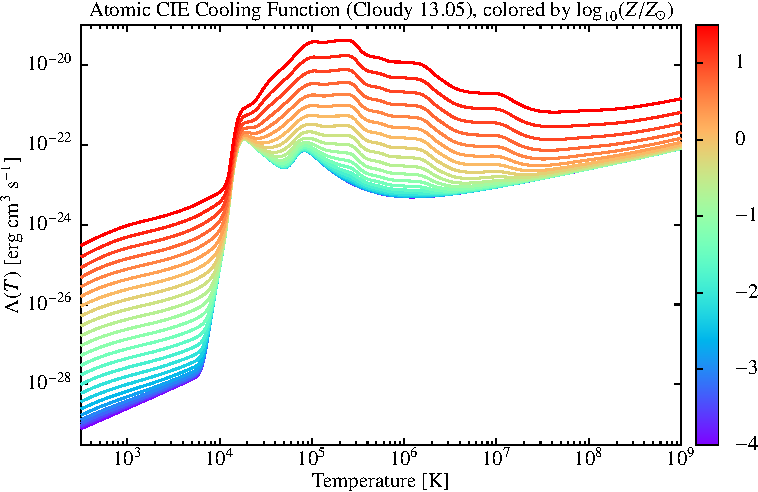
\includegraphics[width=160mm]{../plots/cooling_function_Atomic_CIE_Cloudy.pdf}
 \end{center}
 \caption{Cooling function for atomic gas in collisional ionization equilibrium computed using Cloudy 08.00.}
 \label{fig:atomicCIECloudyCoolingFunction}
\end{figure}

\subsubsection{Cooling Radius}

Additional methods for cooling radius calculations can be added using the {\tt coolingRadiusMethod} directive. The directive should contain a single argument, giving the name of a subroutine to be called to initialize the method. For example, the {\tt simple} method is described by a directive:
\begin{verbatim}
 !# <coolingRadiusMethod>
 !#  <unitName>Cooling_Radius_Simple_Initialize</unitName>
 !# </coolingRadiusMethod>
\end{verbatim}
Here, {\tt Cooling\_Radius\_Simple\_Initialize} is the name of a subroutine which will be called to initialize the method. The initialization subroutine must have the following form:
\begin{verbatim}
  subroutine Method_Initialize(coolingRadiusMethod,Cooling_Radius_Get,Cooling_Radius_Growth_Rate_Get)
    implicit none
    type(varying_string),          intent(in)    :: coolingRadiusMethod
    procedure(),          pointer, intent(inout) :: Cooling_Radius_Get,Cooling_Radius_Growth_Rate_Get
    
    if (coolingRadiusMethod == 'myMethod') then
       Cooling_Radius_Get => My_Method_Get_Procedure
       Cooling_Radius_Growth_Rate_Get => My_Method_Growth_Rate_Get_Procedure
    end if
    return
  end subroutine Method_Initialize
\end{verbatim}
where {\tt myMethod} is the name of this method as will be specified by the {\tt coolingRadiusMethod} input parameter. The procedure pointer {\tt Cooling\_Radius\_Get} must be set to point to a function which returns the cooling function as described below while {\tt Cooling\_Radius\_Growth\_Rate\_Get} should be set to point to a function which returns the rate at which the cooling radius is growing. The initialization subroutine should perform any other tasks required to initialize the module (such as reading parameters etc.).

The cooling radius function must have the form:
\begin{verbatim}
 double precision function Cooling_Radius_Get(thisNode)
    implicit none
    type(treeNode), intent(inout), pointer :: thisNode
    .
    .
    .
    return
 end function Cooling_Radius_Get
\end{verbatim}
The function must return the cooling radius (in units of Mpc) for {\tt thisNode}. The cooling radius growth rate function should have the same template but return the rate at which the cooling radius grows in units of Mpc/Gyr.

Currently defined cooling radius methods are:
\begin{description}
 \item [\hyperlink{cooling.cooling_radius.simple.F90:cooling_radii_simple:cooling_radius_simple}{{\tt simple}}] Computes the cooling radius by seeking the radius at which the time available for cooling equals the cooling time. The growth rate is determined consistently based on the slope of the density profile, the density dependence of the cooling function and the rate at which the time available for cooling is increasing. This method assumes that the cooling time is a monotonic function of radius.
 \item [\hyperlink{cooling.cooling_radius.isothermal_profile.F90:cooling_radii_isothermal:cooling_radius_isothermal}{{\tt isothermal}}] Computes the cooling radius by assuming that the hot gas density profile is an isothermal profile ($\rho(r) \propto r^{-2}$), and that the cooling rate scales as density squared, $\dot{E}\propto \rho^2$, such that the cooling time scales as inverse density, $t_{\rm cool} \propto \rho^{-1}$. Consequently, the cooling radius grows as the square root of the time available for cooling.
\end{description}

\subsubsection{Cooling: Freefall Radius}

Additional methods for freefall radius in cooling calculations can be added using the {\tt freefallRadiusMethod} directive. The directive should contain a single argument, giving the name of a subroutine to be called to initialize the method. For example, the {\tt simple} method is described by a directive:
\begin{verbatim}
 !# <freefallRadiusMethod>
 !#  <unitName>Freefall_Radius_Dark_Matter_Halo_Initialize</unitName>
 !# </freefallRadiusMethod>
\end{verbatim}
Here, {\tt Freefall\_Radius\_Dark\_Matter\_Halo\_Initialize} is the name of a subroutine which will be called to initialize the method. The initialization subroutine must have the following form:
\begin{verbatim}
  subroutine Method_Initialize(freefallRadiusMethod,Freefall_Radius_Get,Freefall_Radius_Growth_Rate_Get)
    implicit none
    type(varying_string),          intent(in)    :: freefallRadiusMethod
    procedure(),          pointer, intent(inout) :: Freefall_Radius_Get,Freefall_Radius_Growth_Rate_Get
    
    if (freefallRadiusMethod == 'myMethod') then
       Freefall_Radius_Get             => My_Method_Get_Procedure
       Freefall_Radius_Growth_Rate_Get => My_Method_Growth_Rate_Get_Procedure
    end if
    return
  end subroutine Method_Initialize
\end{verbatim}
where {\tt myMethod} is the name of this method as will be specified by the {\tt freefallRadiusMethod} input parameter. The procedure pointer {\tt Freefall\_Radius\_Get} must be set to point to a function which returns the freefall radius as described below while {\tt Freefall\_Radius\_Growth\_Rate\_Get} should be set to point to a function which returns the rate at which the freefall radius is growing. The initialization subroutine should perform any other tasks required to initialize the module (such as reading parameters etc.).

The freefall radius function must have the form:
\begin{verbatim}
 double precision function Freefall_Radius_Get(thisNode)
    implicit none
    type(treeNode), intent(inout), pointer :: thisNode
    .
    .
    .
    return
 end function Freefall_Radius_Get
\end{verbatim}
The function must return the freefall radius (in units of Mpc) for {\tt thisNode}. The freefall radius growth rate function should have the same template but return the rate at which the freefall radius grows in units of Mpc/Gyr.

Currently defined freefall radius methods are:
\begin{description}
 \item [\hyperlink{cooling.freefall_radii.dark_matter_halo.F90:freefall_radii_dark_matter_halo:freefall_radius_dark_matter_halo}{{\tt darkMatterHalo}}] Computes the freefall radius by finding the radius in the dark matter halo profile from which a test particle could have free-fallen to zero radius (assuming it began at rest) in the time available for freefall.
\end{description}

\subsubsection{Cooling: Infall Radius}

Additional methods for the infall radius in cooling calculations can be added using the {\tt infallRadiusMethod} directive. The directive should contain a single argument, giving the name of a subroutine to be called to initialize the method. For example, the {\tt coolingRadius} method is described by a directive:
\begin{verbatim}
 !# <infallRadiusMethod>
 !#  <unitName>Infall_Radius_Cooling_Radius_Initialize</unitName>
 !# </infallRadiusMethod>
\end{verbatim}
Here, {\tt Infall\_Radius\_Cooling\_Radius\_Initialize} is the name of a subroutine which will be called to initialize the method. The initialization subroutine must have the following form:
\begin{verbatim}
  subroutine Method_Initialize(infallRadiusMethod,Infall_Radius_Get,Infall_Radius_Growth_Rate_Get)
    implicit none
    type(varying_string),          intent(in)    :: infallRadiusMethod
    procedure(),          pointer, intent(inout) :: Infall_Radius_Get,Infall_Radius_Growth_Rate_Get
    
    if (infallRadiusMethod == 'myMethod') then
       Infall_Radius_Get             => My_Method_Get_Procedure
       Infall_Radius_Growth_Rate_Get => My_Method_Growth_Rate_Get_Procedure
    end if
    return
  end subroutine Method_Initialize
\end{verbatim}
where {\tt myMethod} is the name of this method as will be specified by the {\tt infallRadiusMethod} input parameter. The procedure pointer {\tt Infall\_Radius\_Get} must be set to point to a function which returns the infall radius as described below while {\tt Infall\_Radius\_Growth\_Rate\_Get} should be set to point to a function which returns the rate at which the infall radius is growing. The initialization subroutine should perform any other tasks required to initialize the module (such as reading parameters etc.).

The infall radius function must have the form:
\begin{verbatim}
 double precision function Infall_Radius_Get(thisNode)
    implicit none
    type(treeNode), intent(inout), pointer :: thisNode
    .
    .
    .
    return
 end function Infall_Radius_Get
\end{verbatim}
The function must return the infall radius (in units of Mpc) for {\tt thisNode}, i.e. the radius from which gas in the hot halo that is currently accreting onto the galaxy originated. The infall radius growth rate function should have the same template but return the rate at which the infall radius grows in units of Mpc/Gyr.

Currently defined infall radius methods are:
\begin{description}
 \item [\hyperlink{cooling.infall_radius.cooling_radius.F90:infall_radii_cooling_radius:infall_radius_cooling_radius}{{\tt coolingRadius}}] Assumes that the infall radius equals the cooling radius.
 \item [\hyperlink{cooling.infall_radius.cooling_and_freefall.F90:infall_radii_cooling_freefall:infall_radius_cooling_freefall}{{\tt cooling and freefall}}] Assumes that the infall radius is equal to the smaller of the cooling and freefall radii.
\end{description}

\subsubsection{Cooling Specific Angular Momentum}

Additional methods for calculations of the specific angular momentum of cooling gas can be added using the {\tt coolingSpecificAngularMomentumMethod} directive. The directive should contain a single argument, giving the name of a subroutine to be called to initialize the method. For example, the {\tt simple} method is described by a directive:
\begin{verbatim}
 !# <coolingSpecificAngularMomentumMethod>
 !#  <unitName>Cooling_Specific_AM_Constant_Rotation_Initialize</unitName>
 !# </coolingSpecificAngularMomentumMethod>
\end{verbatim}
Here, {\tt Cooling\_Time\_Simple\_Initialize} is the name of a subroutine which will be called to initialize the method. The initialization subroutine must have the following form:
\begin{verbatim}
  subroutine Method_Initialize(coolingSpecificAngularMomentumMethod,Cooling_Specific_Angular_Momentum_Get)
    implicit none
    type(varying_string),          intent(in)    :: coolingSpecificAngularMomentumMethod
    procedure(),          pointer, intent(inout) :: Cooling_Specific_Angular_Momentum_Get
    
    if (coolingSpecificAngularMomentumMethod == 'myMethod') then
       Cooling_Specific_Angular_Momentum_Get => My_Method_Get_Procedure
    end if
    return
  end subroutine Method_Initialize
\end{verbatim}
where {\tt myMethod} is the name of this method as will be specified by the {\tt coolingSpecificAngularMomentumMethod} input parameter. The procedure pointer {\tt Cooling\_Specific\_Angular\_Momentum\_Get} must be set to point to a function which returns the specific angular momentum of cooling gas. The initialization subroutine should perform any other tasks required to initialize the module (such as reading parameters etc.).

The specific angular momentum of cooling gas function must have the form:
\begin{verbatim}
 double precision function Cooling_Specific_Angular_Momentum_Get(thisNode)
    implicit none
    type(treeNode), intent(inout), pointer :: thisNode
    .
    .
    .
    return
 end function Cooling_Specific_Angular_Momentum_Get
\end{verbatim}
The function must return the specific angular momentum (in units of km/s Mpc) of gas that is cooling in {\tt thisNode}.

Currently defined specific angular momentum of cooling gas methods are:
\begin{description}
 \item [\hyperlink{cooling.specific_angular_momentum.constant_rotation.F90:cooling_specific_angular_momenta_constant_rotation:cooling_specific_angular_momentum_constant_rotation}{{\tt constantRotation}}] Computes the specific angular momentum of the cooling gas based on the cooling radius, mean specific angular momentum and the assumption of a constant mean rotation speed in the cooling gas as a function of radius.
\end{description}

\subsubsection{Cooling Time Available}

Additional methods for the time available for cooling can be added using the {\tt coolingTimeAvailableMethod} directive. The directive should contain a single argument, giving the name of a subroutine to be called to initialize the method. For example, the {\tt White-Frenk} method is described by a directive:
\begin{verbatim}
 !# <coolingTimeAvailableMethod>
 !#  <unitName>Cooling_Time_Available_WF_Initialize</unitName>
 !# </coolingTimeAvailableMethod>
\end{verbatim}
Here, {\tt Cooling\_Time\_Available\_WF\_Initialize} is the name of a subroutine which will be called to initialize the method. The initialization subroutine must have the following form:
\begin{verbatim}
  subroutine Method_Initialize(coolingTimeAvailableMethod,Cooling_Time_Available_Get&
       &,Cooling_Time_Available_Increase_Rate_Get)
    implicit none
    type(varying_string),          intent(in)    :: coolingTimeAvailableMethod
    procedure(),          pointer, intent(inout) :: Cooling_Time_Available_Get,Cooling_Time_Available_Increase_Rate_Get
    
    if (coolingTimeAvailableMethod == 'myMethod') then
      Cooling_Time_Available_Get               => My_Method_Get
      Cooling_Time_Available_Increase_Rate_Get => My_Method_Increase_Rate_Get
    end if
    return
  end subroutine Method_Initialize
\end{verbatim}
where {\tt myMethod} is the name of this method as will be specified by the {\tt coolingTimeAvailableMethod} input parameter. The procedure pointers {\tt Cooling\_Time\_Available\_Get} and {\tt Cooling\_Time\_Available\_Increase\_Rate\_Get} must be set to point to functions which return the time available for cooling and the rate of increase of this time respectively. The initialization subroutine should perform any other tasks required to initialize the module (such as reading parameters etc.).

The cooling time available functions must have the form:
\begin{verbatim}
 double precision function Cooling_Time_Available_Get(thisNode)
    implicit none
    type(treeNode),   intent(inout), pointer :: thisNode
    .
    .
    .
    return
 end function Cooling_Time_Available_Get
\end{verbatim}
The first function must return the time available for cooling (in units of Gyr) for {\tt thisNode}, while the second must return the rate of increase of this time. 

Currently defined cooling time available methods are:
\begin{description}
 \item [\hyperlink{cooling.time_available.White-Frenk.F90:cooling_time_available_white_frenk:cooling_time_available_wf}{{\tt White-Frenk}}] The time available is set to a value between the age of the Universe and the dynamical time of the halo, depending on the interpolating parameter {\tt [coolingTimeAvailableAgeFactor]};
 \item [\hyperlink{cooling.time_available.halo_formation.F90:cooling_times_available_halo_formation:cooling_time_available_halo_formation}{{\tt haloFormation}}] The time available for cooling is set equal to the current time minus the formation time of the halo.
\end{description}

\subsubsection{Cooling Time Available For Freefall}

Additional methods for the time available for freefall in cooling calculations can be added using the {\tt freefallTimeAvailableMethod} directive. The directive should contain a single argument, giving the name of a subroutine to be called to initialize the method. For example, the {\tt haloFormation} method is described by a directive:
\begin{verbatim}
 !# <freefallTimeAvailableMethod>
 !#  <unitName>Freefall_Time_Available_Halo_Formation_Initialize</unitName>
 !# </freefallTimeAvailableMethod>
\end{verbatim}
Here, {\tt Freefall\_Time\_Available\_Halo\_Formation\_Initialize} is the name of a subroutine which will be called to initialize the method. The initialization subroutine must have the following form:
\begin{verbatim}
  subroutine Method_Initialize(freefallTimeAvailableMethod,Freefall_Time_Available_Get&
       &,Freefall_Time_Available_Increase_Rate_Get)
    implicit none
    type(varying_string),          intent(in)    :: freefallTimeAvailableMethod
    procedure(),          pointer, intent(inout) :: Freefall_Time_Available_Get,Freefall_Time_Available_Increase_Rate_Get
    
    if (freefallTimeAvailableMethod == 'myMethod') then
      Freefall_Time_Available_Get               => My_Method_Get
      Freefall_Time_Available_Increase_Rate_Get => My_Method_Increase_Rate_Get
    end if
    return
  end subroutine Method_Initialize
\end{verbatim}
where {\tt myMethod} is the name of this method as will be specified by the {\tt freefallTimeAvailableMethod} input parameter. The procedure pointers {\tt Freefall\_Time\_Available\_Get} and {\tt Freefall\_Time\_Available\_Increase\_Rate\_Get} must be set to point to functions which return the time available for freefal in cooling calculations and the rate of increase of this time respectively. The initialization subroutine should perform any other tasks required to initialize the module (such as reading parameters etc.).

The freefall time available functions must have the form:
\begin{verbatim}
 double precision function Freefall_Time_Available_Get(thisNode)
    implicit none
    type(treeNode),   intent(inout), pointer :: thisNode
    .
    .
    .
    return
 end function Freefall_Time_Available_Get
\end{verbatim}
The first function must return the time available for freefall cooling calculations (in units of Gyr) for {\tt thisNode}, while the second must return the rate of increase of this time. 

Currently defined freefall time available methods are:
\begin{description}
 \item [\hyperlink{cooling.freefall_time_available.halo_formation.F90:freefall_times_available_halo_formation:freefall_time_available_halo_formation}{{\tt haloFormation}}] The time available for cooling is set equal to the current time minus the formation time of the halo.
\end{description}

\subsubsection{Cooling Time}

Additional methods for cooling time calculations can be added using the {\tt coolingTimeMethod} directive. The directive should contain a single argument, giving the name of a subroutine to be called to initialize the method. For example, the {\tt simple} method is described by a directive:
\begin{verbatim}
 !# <coolingTimeMethod>
 !#  <unitName>Cooling_Time_Simple_Initialize</unitName>
 !# </coolingTimeMethod>
\end{verbatim}
Here, {\tt Cooling\_Time\_Simple\_Initialize} is the name of a subroutine which will be called to initialize the method. The initialization subroutine must have the following form:
\begin{verbatim}
  subroutine Method_Initialize(coolingTimeMethod,Cooling_Time_Get,Cooling_Time_Density_Log_Slope_Get,Cooling_Time_Temperature_Log_Slope_Get)
    implicit none
    type(varying_string),          intent(in)    :: coolingTimeMethod
    procedure(),          pointer, intent(inout) :: Cooling_Time_Get,Cooling_Time_Density_Log_Slope_Get,Cooling_Time_Temperature_Log_Slope_Get
    
    if (coolingTimeMethod == 'myMethod') then
       Cooling_Time_Get => My_Method_Get_Procedure
       Cooling_Time_Density_Log_Slope_Get     => My_Method_Density_Log_Slope_Procedure
       Cooling_Time_Temperature_Log_Slope_Get => My_Method_Temperature_Log_Slope_Procedure
    end if
    return
  end subroutine Method_Initialize
\end{verbatim}
where {\tt myMethod} is the name of this method as will be specified by the {\tt coolingTimeMethod} input parameter. The procedure pointer {\tt Cooling\_Time\_Get} must be set to point to a function which returns the cooling function as described below while the other two pointers should point to functions which return the appropriate logarithmic slope. The initialization subroutine should perform any other tasks required to initialize the module (such as reading parameters etc.).

The cooling time function must have the form:
\begin{verbatim}
 double precision function Cooling_Time_Get(temperature,density,abundances,chemicalDensities,radiation)
    implicit none
    double precision,                  intent(in) :: temperature,density
    type(abundancesStructure),         intent(in) :: abundances
    type(chemicalAbundancesStructure), intent(in) :: chemicalDensities
    type(radiationStructure),          intent(in) :: radiation
    .
    .
    .
    return
 end function Cooling_Time_Get
\end{verbatim}
The function must return the cooling time (in units of Gyr) for at the specified {\tt temperature}, {\tt density} and for composition and radiation field as specified by the {\tt abundances}, {\tt chemicalDensities} and {\tt radiation} structures. The logarithmic slope functions should have the same template, but return the logarithmic slope of the cooling time with respect to the appropriate variable instead.

Currently defined cooling time methods are:
\begin{description}
 \item [\hyperlink{cooling.cooling_time.simple.F90:cooling_times_simple:cooling_time_simple}{{\tt simple}}] Compute the cooling time as the ratio of the gas thermal energy density to the volume rate of radiative energy loss. The gas is assumed to have an effective number of degrees of freedom specified by the {\tt coolingTimeSimpleDegreesOfFreedom} parameter.
\end{description}

\subsubsection{Cosmology}\label{sec:CosmologyMethods}

Additional methods for cosmology can be added using the {\tt cosmologyMethod} directive. The directive should contain a single argument, giving the name of a subroutine to be called to initialize the method. For example, the {\tt matter-lambda} method is described by a directive:
\begin{verbatim}
  !# <cosmologyMethod>
  !#  <unitName>Cosmology_Functions_Matter_Lambda_Initialize</unitName>
  !# </cosmologyMethod>
\end{verbatim}
Here, {\tt Cosmology\_Functions\_Matter\_Lambda\_Initialize} is the name of a subroutine which will be called to initialize the method. The initialization subroutine must have the following form:
\begin{verbatim}
  subroutine Method_Initialize(cosmologyMethod,Expansion_Factor_Is_Valid_Get,Cosmic_Time_Is_Valid_Get &
       &,Cosmology_Age_Get,Expansion_Factor_Get,Hubble_Parameter_Get,Early_Time_Density_Scaling_Get  & 
       &,Omega_Matter_Get,Omega_Dark_Energy_Get,Expansion_Rate_Get,Epoch_of_Matter_Dark_Energy_Equality_Get &
       &,Epoch_of_Matter_Domination_Get,Epoch_of_Matter_Curvature_Equality_Get,CMB_Temperature_Get &
       &,Comoving_Distance_Get,Time_From_Comoving_Distance_Get,Comoving_Distance_Conversion)
    implicit none
    type(varying_string),          intent(in)    :: cosmologyMethod
    procedure(),                 pointer, intent(inout) :: Early_Time_Density_Scaling_Get
    procedure(logical),          pointer, intent(inout) :: Expansion_Factor_Is_Valid_Get,Cosmic_Time_Is_Valid_Get
    procedure(double precision), pointer, intent(inout) :: Cosmology_Age_Get ,Expansion_Factor_Get,Hubble_Parameter_Get &
         &,Omega_Matter_Total_Get,Omega_Dark_Energy_Get ,Expansion_Rate_Get,Epoch_of_Matter_Dark_Energy_Equality_Get &
         &,Epoch_of_Matter_Domination_Get ,Epoch_of_Matter_Curvature_Equality_Get,CMB_Temperature_Get,Comoving_Distance_Get&
         &,Time_From_Comoving_Distance_Get,Comoving_Distance_Conversion_Get

    if (cosmologyMethod == 'myMethod') then
       Procedure_Pointer_Get => My_Procedure
       .
       .
       .
    end if
    return
  end subroutine Method_Initialize
\end{verbatim}
where {\tt myMethod} is the name of this method as will be specified by the {\tt cosmologyMethod} input parameter. Numerous procedure pointers are passed in and should be set to point to functions/subroutines that perform cosmological calcalculations as described below. The initialization subroutine should perform any other tasks required to initialize the module (such as reading parameters etc.).

Below are a list of procedure templates for the various procedures required by the cosmology method. After each template a description of what the procedure must do is given.

\begin{verbatim}
   logical function My_Expansion_Factor_Is_Valid(aExpansion)
     implicit none
     double precision, intent(in) :: aExpansion
     .
     .
     .
     return
   end function My_Expansion_Factor_Is_Valid
\end{verbatim}
Should return true if the input expansion factor is valid (e.g. greater than zero and less the the maximum expansion factor for a collapsing universe).

\begin{verbatim}
   logical function My_Cosmic_Time_Is_Valid(time)
     implicit none
     double precision, intent(in) :: time
     .
     .
     .
     return
   end function My_Cosmic_Time_Is_Valid
\end{verbatim}
Should return true if the input cosmic time is valid (e.g. greater than zero and less than the time at the Big Crunch in collapsing universes).

\begin{verbatim}
   double precision function My_Cosmology_Age(aExpansion,collapsingPhase)
     implicit none
     double precision, intent(in)           :: aExpansion
     logical,          intent(in), optional :: collapsingPhase
     .
     .
     .
     return
   end function My_Cosmology_Age
\end{verbatim}
Should return the age (in Gyr) of the universe at a given expansion factor. The {\tt collapsingPhase} argument optionally specififies whether the age during the expanding or collapsing phase is required---if absent then the expanding phase should be assumed.

\begin{verbatim}
   double precision function My_Expansion_Factor(tCosmological)
     implicit none
     double precision, intent(in) :: tCosmological
     .
     .
     .
     return
   end function My_Expansion_Factor
\end{verbatim}
Should return the expansion factor of the universe at the input cosmological time (given in Gyr).

\begin{verbatim}
   double precision function My_Expansion_Rate(aExpansion)
     implicit none
     double precision, intent(in) :: aExpansion
     .
     .
     .
     return
   end function My_Expansion_Rate
\end{verbatim}
Should return the expansion rate, $\dot{a}/a$ (in Gyr$^{-1}$), at the given expansion factor.

\begin{verbatim}
   double precision function My_Hubble_Parameter(tCosmological,aExpansion,collapsingPhase)
     implicit none
     double precision, intent(in), optional :: tCosmological,aExpansion
     logical,          intent(in), optional :: collapsingPhase
     .
     .
     .
     return
   end function My_Hubble_Parameter
\end{verbatim}
Should return the Hubble parameter (in km/s/Mpc) at the given cosmic epoch. The cosmic epoch can be specified as a time since the Big Bang, or an expansion factor (in the expanding phase unless the collapsing phase is specifically requested). Specifying a time and an expansion factor is invalid input, and the routine should abort in such cases.

\begin{verbatim}
   subroutine My_Early_Time_Density_Scaling(dominateFactor,densityPower,aDominant,Omega_Dominant)
     implicit none
     double precision, intent(in)            :: dominateFactor
     double precision, intent(out)           :: densityPower,aDominant
     double precision, intent(out), optional :: Omega_Dominant
     .
     .
     .
     return
   end subroutine My_Early_Time_Density_Scaling
\end{verbatim}
Should compute the epoch, {\tt aDominant}, before which the universe is dominated by a single component (e.g. in a matter and cosmological constant only universe, the epoch before which matter always dominated). The epoch should be such that the component in question dominates over others in density by a factor of {\tt dominateFactor}. The exponent in the density-expansion factor relation for this relation should be returned in {\tt densityPower}. If present, {\tt Omega\_Dominant} should be set to the density of the dominant component (in units of the critical density) at the present day.

\begin{verbatim}
   double precision function My_Epoch_of_Matter_Domination(dominateFactor)
     implicit none
     double precision, intent(in) :: dominateFactor
      .
     .
     .
    return
   end function My_Epoch_of_Matter_Domination
\end{verbatim}
Should return the epoch at which matte dominates the energy density of the universe by the specified factor.

\begin{verbatim}
   double precision function My_Omega_Matter(tCosmological,aExpansion,collapsingPhase)
     implicit none
     double precision, intent(in), optional :: tCosmological,aExpansion
     logical,          intent(in), optional :: collapsingPhase
     .
     .
     .
     return
   end function My_Omega_Matter
\end{verbatim}
Should return $\Omega_{\rm M}$ at the given cosmic epoch. The cosmic epoch can be specified as a time since the Big Bang, or an expansion factor (in the expanding phase unless the collapsing phase is specifically requested). Specifying a time and an expansion factor is invalid input, and the routine should abort in such cases.

\begin{verbatim}
   double precision function My_Omega_Dark_Energy(tCosmological,aExpansion,collapsingPhase)
     implicit none
     double precision, intent(in), optional :: tCosmological,aExpansion
     logical,          intent(in), optional :: collapsingPhase
     .
     .
     .
     return
   end function My_Omega_Dark_Energy
\end{verbatim}
Should return $\Omega_\Lambda$ at the given cosmic epoch. The cosmic epoch can be specified as a time since the Big Bang, or an expansion factor (in the expanding phase unless the collapsing phase is specifically requested). Specifying a time and an expansion factor is invalid input, and the routine should abort in such cases.

\begin{verbatim}
   double precision function My_Epoch_of_Matter_Dark_Energy_Equality(requestType)
     implicit none
     integer, intent(in) :: requestType
     .
     .
     .
     return
   end function My_Epoch_of_Matter_Dark_Energy_Equality
\end{verbatim}
Should return the cosmic epoch at which matter and dark energy have equal energy densities. If {\tt requestType} is {\tt requestTypeTime} (specified in the {\tt Cosmology\_Functions\_Parameters} module) then cosmic time (in Gyr) should be returned, while if it is {\tt requestTypeExpansionFactor} then expansion factor should be returned instead.

\begin{verbatim}
   double precision function My_Epoch_of_Matter_Curvature_Equality(requestType)
     implicit none
     integer, intent(in) :: requestType
     .
     .
     .
     return
   end function My_Epoch_of_Matter_Curvature_Equality
\end{verbatim}
Should return the cosmic epoch at which matter and curvature have equal energy densities. If {\tt requestType} is {\tt requestTypeTime} (specified in the {\tt Cosmology\_Functions\_Parameters} module) then cosmic time (in Gyr) should be returned, while if it is {\tt requestTypeExpansionFactor} then expansion factor should be returned instead.

\begin{verbatim}
   double precision function My_CMB_Temperature(tCosmological,aExpansion,collapsingPhase)
     implicit none
     double precision, intent(in), optional :: tCosmological,aExpansion
     logical,          intent(in), optional :: collapsingPhase
     .
     .
     .
     return
   end function My_CMB_Temperature
\end{verbatim}
Should return the \gls{cmb} temperature (in K) at the given cosmic epoch. The cosmic epoch can be specified as a time since the Big Bang, or an expansion factor (in the expanding phase unless the collapsing phase is specifically requested). Specifying a time and an expansion factor is invalid input, and the routine should abort in such cases.

\begin{verbatim}
   double precision function My_Comoving_Distance(time)
     implicit none
     double precision, intent(in) :: time
     .
     .
     .
     return
   end function My_Comoving_Distance
\end{verbatim}
Should return the comoving distance (in units of Mpc) to the given cosmic time (in units of Gyr).

\begin{verbatim}
   double precision function My_Time_From_Comoving_Distance(comovingDistance)
     implicit none
     double precision, intent(in) :: comovingDistance
     .
     .
     .
     return
   end function My_Time_From_Comoving_Distance
\end{verbatim}
Should return the cosmic time (in units of Gyr) corresponding to the given comoving distance (in units of Mpc).

\begin{verbatim}
   double precision function My_Comoving_Distance_Conversion(output,distanceModulus,redshift)
     implicit none
     integer         , intent(in   ) :: output
     double precision, intent(in   ) :: distanceModulus,redshift
     .
     .
     .
     return
   end function My_Comoving_Distance_Conversion
\end{verbatim}
Should convert between different measures of the cosmological distance to an object. Currently, the only option for {\tt output} is {\tt distanceTypeComoving}, such that the returned value must always be the comoving distance (in units of Mpc). At least one of {\tt distanceModulus} and {\tt redshift} must be supplied---the function mus derive comoving distance from that supplied value.

Currently defined cosmology methods are:
\begin{description}
 \item [{\tt matter-lambda}] Cosmological relations are computed assuming a universe that contains only matter and a cosmological constant.
\end{description}

\subsubsection{Critical Overdensity for Halo Collapse}

Additional methods for the critical linear theory overdensity for halo collapse can be added using the {\tt criticalOverdensityMethod} directive. The directive should contain a single argument, giving the name of a subroutine to be called to initialize the method. For example, the {\tt sphericalTopHat} method is described by a directive:
\begin{verbatim}
  !# <criticalOverdensityMethod>
  !#  <unitName>Spherical_Collape_Delta_Critical_Initialize</unitName>
  !# </criticalOverdensityMethod>
\end{verbatim}
Here, {\tt Spherical\_Collape\_Delta\_Critical\_Initialize} is the name of a subroutine which will be called to initialize the method. The initialization subroutine must have the following form:
\begin{verbatim}
  subroutine Method_Initialize(criticalOverdensityMethod,Critical_Overdensity_Tabulate)
    implicit none
    type(varying_string),          intent(in)    :: criticalOverdensityMethod
    procedure(),          pointer, intent(inout) :: Critical_Overdensity_Tabulate
    
    if (criticalOverdensityMethod.eq.'myMethod') then
       Critical_Overdensity_Tabulate => My_Do_Tabulate
       .
       .
       .
    end if
    return
  end subroutine Method_Initialize
\end{verbatim}
where {\tt myMethod} is the name of this method as will be specified by the {\tt criticalOverdensityMethod} input parameter. The procedure pointer {\tt Critical\_Overdensity\_Tabulate} must be set to point to a subroutine which tabulates the critical overdensity as described below. The initialization subroutine should perform any other tasks required to initialize the module (such as reading parameters etc.).

The tabulation subroutine must have the form:
\begin{verbatim}
   subroutine Critical_Overdensity_Tabulate(time,deltaCritNumberPoints,deltaCritTime,deltaCritDeltaCrit)
    implicit none
    double precision, intent(in)                               :: time
    integer,          intent(out)                              :: deltaCritNumberPoints
    double precision, intent(inout), allocatable, dimension(:) :: deltaCritTime,deltaCritDeltaVirial
    .
    .
    .
    return
   end subroutine Critical_Overdensity_Tabulate
\end{verbatim}
The subroutine must tabulate the critical overdensity in array {\tt deltaCritDeltaVirial()} as a function of wavenumber {\tt deltaCritTime()} (these arrays must be allocated to the correct size, and may be prevously allocated, therefore requiring a deallocation). The number of tabulated points should be returned in {\tt deltaCritNumberPoints}. The subroutine should ensure that the currently requested {\tt time} is within the range of the tabulated function (preferably with some buffer).

Currently defined critical overdensity methods are:
\begin{description}
 \item [{\tt sphericalTopHat}] The critical overdensity is computed for a Universe containing collisionless matter and a cosmological constant following the spherical top hat collapse model (see, for example, \citealt{percival_cosmological_2005}).
 \item [{\tt Kitayama-Suto1996}] The critical overdensity is computed using the fitting formula of \cite{kitayama_semianalytic_1996}, and is therefore valid only for flat cosmological models.
\end{description}

\subsubsection{Critical Overdensity for Halo Collapse: Mass Scaling}

Additional methods for the mass scaling of the critical linear theory overdensity for halo collapse can be added using the {\tt criticalOverdensityMassScalingMethod} directive. The directive should contain a single argument, giving the name of a subroutine to be called to initialize the method. For example, the {\tt warm dark matter} method is described by a directive:
\begin{verbatim}
  !# <criticalOverdensityMassScalingMethod>
  !#  <unitName>Critical_Overdensity_Mass_Scaling_WDM_Initialize</unitName>
  !# </criticalOverdensityMassScalingMethod>
\end{verbatim}
Here, {\tt Critical\_Overdensity\_Mass\_Scaling\_WDM\_Initialize} is the name of a subroutine which will be called to initialize the method. The initialization subroutine must have the following form:
\begin{verbatim}
  subroutine Method_Initialize(criticalOverdensityMassScalingMethod, &
   & Critical_Overdensity_Mass_Scaling_Get,Critical_Overdensity_Mass_Scaling_Gradient_Get)
    implicit none
    type(varying_string),          intent(in)    :: criticalOverdensityMassScalingMethod
    procedure(),          pointer, intent(inout) :: Critical_Overdensity_Mass_Scaling_Get, &
   &                                                Critical_Overdensity_Mass_Scaling_Gradient_Get
    
    if (criticalOverdensityMassScalingMethod == 'myMethod') then
       Critical_Overdensity_Mass_Scaling_Get          => My_Do_Tabulate
       Critical_Overdensity_Mass_Scaling_Gradient_Get => My_Do_Gradient_Tabulate
       .
       .
       .
    end if
    return
  end subroutine Method_Initialize
\end{verbatim}
where {\tt myMethod} is the name of this method as will be specified by the {\tt criticalOverdensityMassScalingMethod} input parameter. The procedure pointers {\tt Critical\_Overdensity\_Mass\_Scaling\_Get} and {\tt Critical\_Overdensity\_Mass\_Scaling\_Gradient\_Get} must be set to point to functions which return the critical overdensity mass scaling and its gradient as described below. The initialization subroutine should perform any other tasks required to initialize the module (such as reading parameters etc.).

The mass scaling function must have the form:
\begin{verbatim}
   double precision function Critical_Overdensity_Mass_Scaling_Get(mass)
    implicit none
    double precision, intent(in) :: mass
    .
    .
    .
    return
   end function Critical_Overdensity_Mass_Scaling_Get
\end{verbatim}
The function should return the factor by which the critical overdensity for collapse at the given {\tt mass} scale (given in units of $M_{\odot}$) differs from that for the case $M\rightarrow\infty$. The mass scaling gradient function should have the same form, but should return the derivative of the scaling with respect to mass.

Currently defined critical overdensity mass scaling methods are:
\begin{description}
 \item [{\tt null}] The critical overdensity is assumed to have no scaling with mass;
 \item [{\tt warm dark matter}] The mass scaling is computed for warm dark matter using a fitting function to the results of \cite{barkana_constraints_2001}.
\end{description}

\subsubsection{Dark Matter Density Profile}

Additional methods for the dark matter density profile can be added using the {\tt darkMatterProfileMethod} directive. The directive should contain a single argument, giving the name of a subroutine to be called to initialize the method. For example, the {\tt NFW} method is described by a directive:
\begin{verbatim}
 !# <darkMatterProfileMethod>
 !#  <unitName>Dark_Matter_Profile_NFW_Initialize</unitName>
 !# </darkMatterProfileMethod>
\end{verbatim}
Here, {\tt Dark\_Matter\_Profile\_NFW\_Initialize} is the name of a subroutine which will be called to initialize the method. The initialization subroutine must have the following form:
\begin{verbatim}
  subroutine Method_Initialize(darkMatterProfileMethod,Dark_Matter_Profile_Density_Get,Dark_Matter_Profile_Energy_Get&
       & ,Dark_Matter_Profile_Energy_Growth_Rate_Get,Dark_Matter_Profile_Rotation_Normalization_Get &
       & ,Dark_Matter_Profile_Radius_from_Specific_Angular_Momentum_Get,Dark_Matter_Profile_Circular_Velocity_Get&
       & ,Dark_Matter_Profile_Potential_Get,Dark_Matter_Profile_Enclosed_Mass_Get,Dark_Matter_Profile_kSpace_Get&
       & ,Dark_Matter_Profile_Freefall_Radius_Get ,Dark_Matter_Profile_Freefall_Radius_Increase_Rate_Get)
    implicit none
    type(varying_string),          intent(in)    :: darkMatterProfileMethod
    procedure(),          pointer, intent(inout) :: Dark_Matter_Profile_Density_Get,Dark_Matter_Profile_Energy_Get,Dark_Matter_Profile_Energy_Growth_Rate_Get&
         &,Dark_Matter_Profile_Rotation_Normalization_Get,Dark_Matter_Profile_Radius_from_Specific_Angular_Momentum_Get&
         &,Dark_Matter_Profile_Circular_Velocity_Get,Dark_Matter_Profile_Potential_Get,Dark_Matter_Profile_Enclosed_Mass_Get&
         &,Dark_Matter_Profile_kSpace_Get,Dark_Matter_Profile_Freefall_Radius_Get&
         &,Dark_Matter_Profile_Freefall_Radius_Increase_Rate_Get

    if (darkMatterProfileMethod == 'myMethod') then
       Dark_Matter_Profile_Density_Get                               => My_Dark_Matter_Profile_Density
       Dark_Matter_Profile_Energy_Get                                => My_Dark_Matter_Profile_Energy
       Dark_Matter_Profile_Energy_Growth_Rate_Get                    => My_Dark_Matter_Profile_Energy_Growth_Rate
       Dark_Matter_Profile_Rotation_Normalization_Get                => My_Dark_Matter_Profile_Rotation_Normalization
       Dark_Matter_Profile_Radius_from_Specific_Angular_Momentum_Get => My_Radius_from_Specific_Angular_Momentum
       Dark_Matter_Profile_Circular_Velocity_Get                     => My_Dark_Matter_Profile_Circular_Velocity
       Dark_Matter_Profile_Potential_Get                             => My_Dark_Matter_Profile_Potential
       Dark_Matter_Profile_Enclosed_Mass_Get                         => My_Dark_Matter_Profile_Enclosed_Mass
       Dark_Matter_Profile_kSpace_Get                                => My_Dark_Matter_Profile_kSpace
       Dark_Matter_Profile_Freefall_Radius_Get                       => My_Dark_Matter_Profile_Freefall_Radius
       Dark_Matter_Profile_Freefall_Radius_Increase_Rate_Get         => My_Dark_Matter_Profile_Freefall_Radius_Increase_Rate
       .
       .
       .
    end if
    return
  end subroutine Method_Initialize
\end{verbatim}
where {\tt myMethod} is the name of this method as will be specified by the {\tt darkMatterProfileMethod} input parameter. The procedure pointers must be set to point to functions which return properties of the dark matter density profile as described below. The initialization subroutine should perform any other tasks required to initialize the module (such as reading parameters etc.).

The density, enclosed mass, potential and circular velocity functions must have the form:
\begin{verbatim}
  double precision function My_Dark_Matter_Profile_Property(thisNode,radius)
    implicit none
    type(treeNode),   intent(inout), pointer :: thisNode
    double precision, intent(in)             :: radius
    .
    .
    .
    return
  end function My_Dark_Matter_Profile_Property
\end{verbatim}
These functions should compute and return the density (in units of $M_\odot$ Mpc$^{-3}$), enclosed dark matter mass (in units of $M_\odot$), gravitational potential (in units of (km/s)$^2$) and circular velocity (in units of km/s) due to dark matter at the given {\tt radius} (in units of Mpc) for {\tt thisNode} respectively.

The freefall radius functions must have the form:
\begin{verbatim}
  double precision function My_Dark_Matter_Profile_Property(thisNode,time)
    implicit none
    type(treeNode),   intent(inout), pointer :: thisNode
    double precision, intent(in)             :: time
    .
    .
    .
    return
  end function My_Dark_Matter_Profile_Property
\end{verbatim}
These functions should compute and return the freefall radius (in units of Mpc), or its growth rate given a {\tt time} available for freefall (in Gyr) for {\tt thisNode} respectively.

The energy, energy growth rate and rotation velocity normalization functions must have the form:
\begin{verbatim}
  double precision function My_Dark_Matter_Profile_Property(thisNode)
    implicit none
    type(treeNode),   intent(inout), pointer :: thisNode
    .
    .
    .
    return
  end function My_Dark_Matter_Profile_Property
\end{verbatim}
The energy functions should compute and return the energy (potential plus kinetic; in units of $M_\odot$ (km/s)$^2$) of the dark matter halo out to the virial radius of {\tt thisNode} and the rate of change of that energy (in units of $M_\odot$ (km/s)$^2$ Gyr$^{-1}$) respectively. The rotation normalization function should compute and return the normalization between rotation speed and mean specific angular momentum (in units of Mpc$^{-1}$) of {\tt thisNode} assuming that the dark matter halo rotates at the same velocity at all radii.

Finally, the radius from specific angular momentum function must have the form:
\begin{verbatim}
  double precision function My_Dark_Matter_Profile_Radius_From_Specific_Angular_Momentum(thisNode,specificAngularMomentum)
    implicit none
    type(treeNode),   intent(inout), pointer :: thisNode
    double precision, intent(in)             :: specificAngularMomentum
    .
    .
    .
    return
  end function My_Dark_Matter_Profile_Radius_From_Specific_Angular_Momentum
\end{verbatim}
This function should compute and return the radius (in units of Mpc) in {\tt thisNode} at which a circular orbit would have the given {\tt specificAngularMomentum} (in units of km/s Mpc).

The ``kSpace'' function must have the form:
\begin{verbatim}
  double precision function My_Dark_Matter_Profile_kSpace(thisNode,wavenumber)
    implicit none
    type(treeNode),   intent(inout), pointer :: thisNode
    double precision, intent(in)             :: wavenumber
    .
    .
    .
    return
  end function My_Dark_Matter_Profile_kSpace
\end{verbatim}
This function should compute and return the Fourier transform of the dark matter halo density profile (normalized to unity at small wavenumber---as defined in \citealt{cooray_halo_2002}) for {\tt thisNode} at the given {\tt wavenumber} (specified in Mpc$^{-1}$).

Currently defined dark matter density profile methods are:
\begin{description}
 \item [{\tt Isothermal}] The density profile is a singular isothermal sphere;
 \item [{\tt NFW}] The density profile proposed by \cite{navarro_universal_1997}\index{Navarro-Frenk-White profile}\index{density profile!Navarro-Frenk-White}.
 \item [{\tt Einasto}] The Einasto density profile, described, for example, by \cite{cardone_spherical_2005}\index{Einasto profile}\index{density profile!Einasto}.
\end{description}

\subsubsection{Dark Matter Halo Mass Accretion History}\index{dark matter halo!mass accretion history}\index{mass accretion history!dark matter halo}\label{sec:HaloMassAccretionHistory}

Additional methods for dark matter halo mass accretion histories can be added using the {\tt darkMatterAccretionHistoryMethod} directive. The directive should contain a single argument, giving the name of a subroutine to be called to initialize the method. For example, the {\tt Zhao2009} method is described by a directive:
\begin{verbatim}
 !# <darkMatterAccretionHistoryMethod>
 !#  <unitName>Dark_Matter_Mass_Accretion_Zhao2009_Initialize</unitName>
 !# </darkMatterAccretionHistoryMethod>
\end{verbatim}
Here, {\tt Dark\_Matter\_Mass\_Accretion\_Zhao2009\_Initialize} is the name of a subroutine which will be called to initialize the method. The initialization subroutine must have the following form:
\begin{verbatim}
  subroutine Method_Initialize(darkMatterAccretionHistoryMethod,Dark_Matter_Halo_Mass_Accretion_Time_Get)
    implicit none
    type(varying_string),          intent(in)    :: darkMatterAccretionHistoryMethod
    procedure(),          pointer, intent(inout) :: Dark_Matter_Halo_Mass_Accretion_Time_Get
    
    if (darkMatterAccretionHistoryMethod == 'myMethod') then
       Dark_Matter_Halo_Mass_Accretion_Time_Get => My_Time_Get
       .
       .
       .
    end if
    return
  end subroutine Method_Initialize
\end{verbatim}
where {\tt myMethod} is the name of this method as will be specified by the {\tt darkMatterAccretionHistoryMethod} input parameter. The procedure pointer {\tt Dark\_Matter\_Halo\_Mass\_Accretion\_Time\_Get} must be set to point to a function which returns the time at which a given mass is reached in the mass accretion history. The initialization subroutine should perform any other tasks required to initialize the module (such as reading parameters etc.).

The time function must have the form:
\begin{verbatim}
  double precision function My_Dark_Matter_Halo_Mass_Accretion_Time(baseNode,nodeMass)
    implicit none
    type(treeNode),   intent(inout), pointer :: baseNode
    double precision, intent(in)             :: nodeMass
    .
    .
    .
    return
  end function My_Dark_Matter_Halo_Mass_Accretion_Time
\end{verbatim}
The function should compute and return the time at which the mass accretion history of {\tt baseNode} reaches the specified {\tt nodeMass}.

Currently defined mass accretion history methods are:
\begin{description}
 \item [{\tt Wechsler2002}] Uses the fitting function from \cite{wechsler_concentrations_2002} to compute the mass accretion history. If {\tt [accretionHistoryWechslerFormationRedshiftCompute]} is set to true then the formation redshift for each history is set sing the method of \cite{bullock_profiles_2001}, otherwise it can be set directly via the {\tt [accretionHistoryWechslerFormationRedshift]} parameter;
 \item [{\tt Zhao2009}] Uses the algorithm of \cite{zhao_accurate_2009} to compute the mass accretion history.
\end{description}

\subsubsection{Dark Matter Density Profile Concentration}

Additional methods for the dark matter density profile concentration can be added using the {\tt darkMatterConcentrationMethod} directive. The directive should contain a single argument, giving the name of a subroutine to be called to initialize the method. For example, the {\tt Gao2008} method is described by a directive:
\begin{verbatim}
 !# <darkMatterConcentrationMethod>
 !#  <unitName>Dark_Matter_Concentrations_Gao20008_Initialize</unitName>
 !# </darkMatterConcentrationMethod>
\end{verbatim}
Here, {\tt Dark\_Matter\_Concentrations\_Gao20008\_Initialize} is the name of a subroutine which will be called to initialize the method. The initialization subroutine must have the following form:
\begin{verbatim}
  subroutine Method_Initialize(darkMatterConcentrationMethod,Dark_Matter_Profile_Concentration_Get)
    implicit none
    type(varying_string),          intent(in)    :: darkMatterConcentrationMethod
    procedure(),          pointer, intent(inout) :: Dark_Matter_Profile_Concentration_Get
    
    if (darkMatterConcentrationMethod == 'myMethod') then
       Dark_Matter_Profile_Concentration_Get => My_Concentration_Get
       .
       .
       .
    end if
    return
  end subroutine Method_Initialize
\end{verbatim}
where {\tt myMethod} is the name of this method as will be specified by the {\tt darkMatterConcentrationMethod} input parameter. The procedure pointer {\tt Dark\_Matter\_Profile\_Concentration\_Get} must be set to point to a function which returns the concentration of a node. The initialization subroutine should perform any other tasks required to initialize the module (such as reading parameters etc.).

The concentration function must have the form:
\begin{verbatim}
  double precision function My_Dark_Matter_Profile_Concentration(thisNode)
    implicit none
    type(treeNode), intent(inout), pointer :: thisNode
    .
    .
    .
    return
  end function My_Dark_Matter_Profile_Concentration
\end{verbatim}
The function should compute and return the concentration for {\tt thisNode}.

Currently defined darl matter profile concentration methods are:
\begin{description}
 \item [{\tt NFW1996}] The concentration is computed using the algorithm given by \cite{navarro_structure_1996};
 \item [{\tt Gao2008}] The concentration is computed using a fitting function from \cite{gao_redshift_2008};
 \item [{\tt Zhao2009}] The concentration is computed using a fitting function from \cite{zhao_accurate_2009}. Halo formation times (as defined by \citealt{zhao_accurate_2009}) are computed directly from the merger tree branch associated with each node. Where the tree does not exist or has insufficient resolution to contain the merging time the merging time will be found by extrapolation of the earliest resolved progenitor halo using the selected mass accretion history method (see \S\ref{sec:HaloMassAccretionHistory});
 \item [{\tt Munoz-Cuartas2011}] The concentration is computed using a fitting function from \cite{munoz-cuartas_redshift_2011};
 \item [{\tt Prada2011}] The concentration is computed using a fitting function from \cite{prada_halo_2011};
\end{description}

\subsubsection{Dark Matter Density Profile Shape}\label{sec:darkMatterProfileShape}

Additional methods for the dark matter density profile shape paramter can be added using the {\tt darkMatterShapeMethod} directive. The directive should contain a single argument, giving the name of a subroutine to be called to initialize the method. For example, the {\tt Gao2008} method is described by a directive:
\begin{verbatim}
 !# <darkMatterShapeMethod>
 !#  <unitName>Dark_Matter_Shapes_Gao20008_Initialize</unitName>
 !# </darkMatterShapeMethod>
\end{verbatim}
Here, {\tt Dark\_Matter\_Shapes\_Gao20008\_Initialize} is the name of a subroutine which will be called to initialize the method. The initialization subroutine must have the following form:
\begin{verbatim}
  subroutine Method_Initialize(darkMatterShapeMethod,Dark_Matter_Profile_Shape_Get)
    implicit none
    type(varying_string),          intent(in)    :: darkMatterShapeMethod
    procedure(),          pointer, intent(inout) :: Dark_Matter_Profile_Shape_Get
    
    if (darkMatterShapeMethod == 'myMethod') then
       Dark_Matter_Profile_Shape_Get => My_Shape_Get
       .
       .
       .
    end if
    return
  end subroutine Method_Initialize
\end{verbatim}
where {\tt myMethod} is the name of this method as will be specified by the {\tt darkMatterShapeMethod} input parameter. The procedure pointer {\tt Dark\_Matter\_Profile\_Shape\_Get} must be set to point to a function which returns the shape parameter of a node. The initialization subroutine should perform any other tasks required to initialize the module (such as reading parameters etc.).

The shape parameter function must have the form:
\begin{verbatim}
  double precision function My_Dark_Matter_Profile_Shape(thisNode)
    implicit none
    type(treeNode), intent(inout), pointer :: thisNode
    .
    .
    .
    return
  end function My_Dark_Matter_Profile_Shape
\end{verbatim}
The function should compute and return the shape parameter for {\tt thisNode}.

Currently defined darl matter profile shape parameter methods are:
\begin{description}
 \item [{\tt Gao2008}] The shape parameter is computed using a fitting function from \cite{gao_redshift_2008} - see \S\ref{sec:DarkMatterProfileShape} for details.
\end{description}

\subsubsection{Dark Matter Halo Spin Distribution}\label{sec:HaloSpinDistribution}\index{dark matter halo!spin!distribution}\index{spin!dark matter halo}

Additional methods for the dark matter density profile concentration can be added using the {\tt haloSpinDistributionMethod} directive. The directive should contain a single argument, giving the name of a subroutine to be called to initialize the method. For example, the {\tt Gao2008} method is described by a directive:
\begin{verbatim}
 !# <haloSpinDistributionMethod>
 !#  <unitName>Halo_Spin_Distribution_Bett2007_Initialize</unitName>
 !# </haloSpinDistributionMethod>
\end{verbatim}
Here, {\tt Halo\_Spin\_Distribution\_Bett2007\_Initialize} is the name of a subroutine which will be called to initialize the method. The initialization subroutine must have the following form:
\begin{verbatim}
  subroutine Method_Initialize(haloSpinDistributionMethod,Halo_Spin_Sample_Get)
    implicit none
    type(varying_string),          intent(in)    :: haloSpinDistributionMethod
    procedure(),          pointer, intent(inout) :: Halo_Spin_Sample_Get
    
    if (haloSpinDistributionMethod == 'myMethod') then
       Halo_Spin_Sample_Get => My_Spin_Sample_Get
       .
       .
       .
    end if
    return
  end subroutine Method_Initialize
\end{verbatim}
where {\tt myMethod} is the name of this method as will be specified by the {\tt haloSpinDistributionMethod} input parameter. The procedure pointer {\tt Halo\_Spin\_Sample\_Get} must be set to point to a function which returns a spin parameter drawn at random from a distribution. The initialization subroutine should perform any other tasks required to initialize the module (such as reading parameters etc.).

The spin parameter function must have the form:
\begin{verbatim}
  double precision function My_Spin_Distribution_Sample(thisNode)
    implicit none
    type(treeNode), intent(inout), pointer :: thisNode
    .
    .
    .
    return
  end function My_Spin_Distribution_Sample
\end{verbatim}
The function should compute and return a spin parameter for {\tt thisNode} drawn at random from a distribution.

Currently defined spin distribution methods are:
\begin{description}
 \item [{\tt lognormal}] The spin is drawn from a lognormal distribution with median {\tt [lognormalSpinDistributionMedian]} and width {\tt [lognormalSpinDistributionSigma]}.
 \item [{\tt Bett2007}] The spin is drawn from the distribution found by \cite{bett_spin_2007}. The $\lambda_0$ and $\alpha$ parameter of Bett et al.'s distribution are set by the {\tt [spinDistributionBett2007Lambda0]} and {\tt [spinDistributionBett2007Alpha]} input parameters.
 \item [{\tt deltaFunction}] The spin is drawn from a delta function distribution, i.e. a value equal to {\tt [deltaFunctionSpinDistributionSpin]} is always returned.
\end{description}

\subsubsection{Dark Matter Halo Mass Loss Rates}\label{sec:HaloMassLossRates}\index{dark matter halo!mass loss}\index{mass loss!dark matter halo}

Additional methods for dark matter halo mass loss rates can be added using the {\tt darkMatterHaloMassLossRateMethod} directive. The directive should contain a single argument, giving the name of a subroutine to be called to initialize the method. For example, the {\tt van den Bosch 2005} method is described by a directive:
\begin{verbatim}
 !# <darkMatterHaloMassLossRateMethod>
 !#  <unitName>Dark_Matter_Halos_Mass_Loss_Rate_vanDenBosch_Initialize</unitName>
 !# </darkMatterHaloMassLossRateMethod>
\end{verbatim}
Here, {\tt Dark\_Matter\_Halos\_Mass\_Loss\_Rate\_vanDenBosch\_Initialize} is the name of a subroutine which will be called to initialize the method. The initialization subroutine must have the following form:
\begin{verbatim}
  subroutine Method_Initialize(darkMatterHaloMassLossRateMethod,Dark_Matter_Halos_Mass_Loss_Rate_Get)
    implicit none
    type(varying_string),          intent(in)    :: darkMatterHaloMassLossRateMethod
    procedure(),          pointer, intent(inout) :: Dark_Matter_Halos_Mass_Loss_Rate_Get
    
    if (darkMatterHaloMassLossRateMethod == 'myMethod') then
       Dark_Matter_Halos_Mass_Loss_Rate_Get => My_Mass_Loss_Rate_Get
       .
       .
       .
    end if
    return
  end subroutine Method_Initialize
\end{verbatim}
where {\tt myMethod} is the name of this method as will be specified by the {\tt darkMatterHaloMassLossRateMethod} input parameter. The procedure pointer {\tt Dark\_Matter\_Halos\_Mass\_Loss\_Rate\_Get} must be set to point to a function which returns a spin parameter drawn at random from a distribution. The initialization subroutine should perform any other tasks required to initialize the module (such as reading parameters etc.).

The mass loss rate function must have the form:
\begin{verbatim}
  double precision function My_Mass_Loss_Rate(thisNode)
    implicit none
    type(treeNode), intent(inout), pointer :: thisNode
    .
    .
    .
    return
  end function My_Mass_Loss_Rate
\end{verbatim}
The function should compute and return the mass loss rate from {\tt thisNode} in units of $M_\odot/$Gyr.

Currently defined halo mass loss rate methods are:
\begin{description}
 \item [{\tt null}] Always returns zero mass loss rate.
 \item [{\tt vanDenBosch2005}] Uses the algorithm of \cite{van_den_bosch_mass_2005} to compute the mass loss rate.
\end{description}

\subsubsection{Excursion Set Barrier}\label{sec:excursionSetBarrierMethod}

Additional methods for the excursion set barrier can be added using the {\tt excursionSetBarrierMethod} directive. The directive should contain a single argument, giving the name of a subroutine to be called to initialize the method. For example, the {\tt linear} method is described by a directive:
\begin{verbatim}
 !# <excursionSetBarrierMethod>
 !#  <unitName>Excursion_Sets_Barriers_Linear_Initialize</unitName>
 !# </excursionSetBarrierMethod>
\end{verbatim}
Here, {\tt Excursion\_Sets\_Barriers\_Linear\_Initialize} is the name of a subroutine which will be called to initialize the method. The initialization subroutine must have the following form:
\begin{verbatim}
  subroutine Method_Initialize(excursionSetBarrierMethodExcursion_Sets_Barrier_Get,Excursion
_Sets_Barrier_Gradient_Get,barrierName)
    implicit none
    type     (varying_string  ),         intent(in   ) :: excursionSetBarrierMethod
    procedure(double precision),pointer, intent(inout) :: Excursion_Sets_Barrier_Get,Excursion_Sets_Barrier_Gradient
_Get
    type(varying_string),                intent(inout) :: barrierName

    if (excursionSetBarrierMethod == 'myMethod') then
      Excursion_Sets_Barrier_Get          => My_Barrier
      Excursion_Sets_Barrier_Gradient_Get => My_Barrier_Gradient
      barrierName=barrierName//":myLabel"
    end if
    return
  end subroutine Method_Initialize
\end{verbatim}
where {\tt myMethod} is the name of this method as will be specified by the {\tt excursionSetBarrierMethod} input parameter. The procedure pointers {\tt Excursion\_Sets\_Barrier\_Get}, and {\tt Excursion\_Sets\_Barrier\_Gradient\_Get} must be set to point functions which return the barrier and its gradient respectively, as described below. The initialization subroutine should also append a descriptive label to the {\tt barrierName} argument. The initialization subroutine should perform any other tasks required to initialize the module (such as reading parameters etc.).

The barrier and barrier gradient functions must have the form:
\begin{verbatim}
 double precision function Excursion_Sets_Barrier(variance,time)
    implicit none
    double precision, intent(in) :: variance,time
    .
    .
    .
    return
 end function Excursion_Sets_Barrier
\end{verbatim}
The barrier function must return the barrier at the specified {\tt variance} and {\tt time}, while the barrier gradient function should return the derivative with respect to variance of the same barrier.

Currently defined excursion set barrier methods are:
\begin{description}
 \item [{\tt linear}] A linear ($1^{\rm st}$-order polynomial) barrier;
  \item [{\tt quadratic}] A quadratic ($2^{\rm nd}$-order polynomial);
  \item [{\tt criticalOverdensity}] A barrier equal to the critical overdensity for halo collapse.
\end{description}

\subsubsection{Excursion Set Barrier First Crossing Distribution}\label{sec:excursionSetFirstCrossingMethod}

Additional methods for the excursion set barrier first crossing distribution can be added using the {\tt excursionSetFirstCrossingMethod} directive. The directive should contain a single argument, giving the name of a subroutine to be called to initialize the method. For example, the {\tt linearBarrier} method is described by a directive:
\begin{verbatim}
 !# <excursionSetFirstCrossingMethod>
 !#  <unitName>Excursion_Sets_First_Crossing_Linear_Barrier_Initialize</unitName>
 !# </excursionSetFirstCrossingMethod>
\end{verbatim}
Here, {\tt Excursion\_Sets\_First\_Crossing\_Linear\_Barrier\_Initialize} is the name of a subroutine which will be called to initialize the method. The initialization subroutine must have the following form:
\begin{verbatim}
  subroutine Method_Initialize(excursionSetFirstCrossingMethod,Excursion_Sets_First_Crossing_Probability_Get&
         &,Excursion_Sets_First_Crossing_Rate_Get,Excursion_Sets_Non_Crossing_Rate_Get)
    implicit none
    type     (varying_string  ),         intent(in   ) :: excursionSetFirstCrossingMethod
    procedure(double precision),pointer, intent(inout) :: Excursion_Sets_First_Crossing_Probability_Get&
         &,Excursion_Sets_First_Crossing_Rate_Get,Excursion_Sets_Non_Crossing_Rate_Get
    
    if (excursionSetFirstCrossingMethod == 'myMethod') then
       Excursion_Sets_First_Crossing_Probability_Get => My_First_Crossing_Probability
       Excursion_Sets_First_Crossing_Rate_Get        => My_First_Crossing_Rate
       Excursion_Sets_Non_Crossing_Rate_Get          => My_Non_Crossing_Rate
    end if
    return
  end subroutine Method_Initialize
\end{verbatim}
where {\tt myMethod} is the name of this method as will be specified by the {\tt excursionSetFirstCrossingMethod} input parameter. The procedure pointers {\tt Excursion\_Sets\_First\_Crossing\_Probability\_Get}, {\tt Excursion\_Sets\_First\_Crossing\_Rate\_Get}, and {\tt Excursion\_Sets\_Non\_Crossing\_Rate\_Get} must be set to point functions which return the first crossing probability, first crossing probability rate and noncrossing rate as described below. The initialization subroutine should perform any other tasks required to initialize the module (such as reading parameters etc.).

The first crossing probability function must have the form:
\begin{verbatim}
 double precision function Excursion_Sets_First_Crossing_Probability(variance,time)
    implicit none
    double precision, intent(in) :: variance,time
    .
    .
    .
    return
 end function Excursion_Sets_First_Crossing_Probability
\end{verbatim}
The function must return the first crossing probability per unit variance at the specified {\tt variance} and {\tt time}.

The first crossing probability rate function must have the form:
\begin{verbatim}
 double precision function Excursion_Sets_First_Crossing_Rate(variance,varianceProgenitor,time)
    implicit none
    double precision, intent(in) :: variance,varianceProgenitor,time
    .
    .
    .
    return
 end function Excursion_Sets_First_Crossing_Rate
\end{verbatim}
The function must return the rate of first crossing per unit variance at the specified {\tt variance} and {\tt time} for a progenitor of the specified {\tt varianceProgenitor}.

The non-crossing probability rate function must have the form:
\begin{verbatim}
 double precision function Excursion_Sets_First_Non_Crossing_Rate(variance,time)
    implicit none
    double precision, intent(in) :: variance,time
    .
    .
    .
    return
 end function Excursion_Sets_First_Non_Crossing_Rate
\end{verbatim}
The function must return the rate of trajectories which never cross the barrier at the specified {\tt variance} and {\tt time}..

Currently defined excursion set barrier first crossing methods are:
\begin{description}
 \item [{\tt linearBarrier}] Assumes the solution for a linear barrier;
 \item [{\tt Farahi}] Solves the first crossing problem using the methodology of \cite{benson_dark_2012};
 \item [{\tt ZhangHui2006}] Solves the first crossing problem using the methodology of \cite{zhang_random_2006};
 \item [{\tt ZhangHui2006HighOrder}] Solves the first crossing problem using a higher order extension of the methodology of \cite{zhang_random_2006}.
\end{description}

\subsubsection{Excursion Set Barrier Remapping}\label{sec:excursionSetBarrierRemapInitialize}

Additional methods for the excursion set barrier can be added using the {\tt excursionSetBarrierRemapInitialize} directive. The directive should contain a single argument, giving the name of a subroutine to be called to initialize the method. For example, the {\tt scale} method is described by a directive:
\begin{verbatim}
 !# <excursionSetBarrierRemapInitialize>
 !#  <unitName>Excursion_Sets_Barriers_Remap_Scale_Initialize</unitName>
 !# </excursionSetBarrierRemapInitialize>
\end{verbatim}
Here, {\tt Excursion\_Sets\_Barriers\_Remap\_Scale\_Initialize} is the name of a subroutine which will be called to initialize the method. The initialization subroutine must have the following form:
\begin{verbatim}
  subroutine Method_Initialize(excursionSetBarrierRemapMethods,barrierName, &
  & ratesCalculation,matchedCount)
    implicit none
    type(varying_string), intent(in   ), dimension(:) :: excursionSetBarrierRemapMethods
    type(varying_string), intent(inout)               :: barrierName
    logical             , intent(in   )               :: ratesCalculation
    integer             , intent(inout)               :: matchedCount

    if (any(excursionSetBarrierRemapMethods == 'myMethod')) then
       position=-1
       do i=1,size(excursionSetBarrierRemapMethods)
          if (excursionSetBarrierRemapMethods(i) == 'myMethod') then
             position=i
             exit
          end if
       end do
       if (ratesCalculation) then
          methodRatesPosition=position
       else
          methodPosition     =position
       end if
       matchedCount=matchedCount+1
       barrierName=barrierName//":myLabel"
    end if
    return
  end subroutine Method_Initialize
\end{verbatim}
where {\tt myMethod} is the name of this method as will be specified by the {\tt excursionSetBarrierRemapMethods} input parameter. The initialization subroutine should identify the position of the matched method in the {\tt excursionSetBarrierRemapMethods()} array and record that it is active for standard barrier calculations ({\tt ratesCalculation}$=${\tt false}) or for barriers used in crossing rate calculations ({\tt ratesCalculation}$=${\tt true}). It should also increment the {\tt matchedCount} argument (to allow checking that all specified barriers were matched) and append a descriptive label to the{\tt barrierName} argument. The initialization subroutine should perform any other tasks required to initialize the module (such as reading parameters etc.).

The method must provide a subroutine to compute remapping of the barrier as follows:
\begin{verbatim}
  !# <excursionSetBarrierRemap>
  !#  <unitName>Method_Barrier_Remap</unitName>
  !# </excursionSetBarrierRemap>
  subroutine Method_Barrier_Remap(barrier,variance,time,ratesCalculation,iRemap)
    implicit none
    double precision, intent(inout) :: barrier
    double precision, intent(in   ) :: variance,time
    logical         , intent(in   ) :: ratesCalculation
    integer         , intent(in   ) :: iRemap

    if ((ratesCalculation.and.iRemap == methodRatesPosition).or.(.not.ratesCalculation.and.iRemap == methodPosition)) then
     ! Do remapping.
     .
     .
     .
    end if
    return
  end subroutine Method_Barrier_Remap
\end{verbatim}
and a subroutine to compute remapping of the barrier gradient as follows:
\begin{verbatim}
  !# <excursionSetBarrierRemapGradient>
  !#  <unitName>Method_Barrier_Gradient_Remap</unitName>
  !# </excursionSetBarrierRemapGradient>
  subroutine Method_Barrier_Gradient_Remap(barrier,barrierGradient,variance,time,ratesCalculation,iRemap)
    implicit none
    double precision, intent(inout) :: barrier,barrierGradient
    double precision, intent(in   ) :: variance,time
    logical         , intent(in   ) :: ratesCalculation
    integer         , intent(in   ) :: iRemap

    if ((ratesCalculation.and.iRemap == methodRatesPosition).or.(.not.ratesCalculation.and.iRemap == methodPosition)) then
     ! Do remapping.
     .
     .
     .
    end if
    return
  end subroutine Method_Barrier_Gradient_Remap
\end{verbatim}

Currently defined excursion set barrier remapping methods are:
\begin{description}
 \item [{\tt null}] A null method which leaves the barrier unchanged;
 \item [{\tt scale}] Scales the barrier by a multiplicative factor;
 \item [{\tt Sheth-Mo-Tormen}] Remaps the barrier according to the algorithm of \cite{sheth_ellipsoidal_2001}.
\end{description}

\subsubsection{Galactic Component Radii Solver}\label{sec:galactic_radii_solvers}

Additional methods for solving for radii of galactic components can be added using the {\tt galacticStructureRadiusSolverMethod} directive. The directive should contain a single argument, giving the name of a subroutine to be called to initialize the method. For example, the {\tt simple} method is described by a directive:
\begin{verbatim}
 !# <galacticStructureRadiusSolverMethod>
 !#  <unitName>Galactic_Structure_Radii_Simple_Initialize</unitName>
 !# </galacticStructureRadiusSolverMethod>
\end{verbatim}
Here, {\tt Galactic\_Structure\_Radii\_Simple\_Initialize} is the name of a subroutine which will be called to initialize the method. The initialization subroutine must have the following form:
\begin{verbatim}
  subroutine Method_Initialize(galacticStructureRadiusSolverMethod,Galactic_Structure_Radii_Solve_Do)
    implicit none
    type(varying_string),          intent(in)    :: galacticStructureRadiusSolverMethod
    procedure(),          pointer, intent(inout) :: Galactic_Structure_Radii_Solve_Do
    
    if (galacticStructureRadiusSolverMethod == 'myMethod') Galactic_Structure_Radii_Solve_Do => My_Method_Do_Procedure
    return
  end subroutine Method_Initialize
\end{verbatim}
where {\tt myMethod} is the name of this method as will be specified by the {\tt galacticStructureRadiusSolverMethod} input parameter. The procedure pointer {\tt Galactic\_Structure\_Radii\_Solve\_Do} must be set to point to a subroutine which solves for the radii of components in a node as described below. The initialization subroutine should perform any other tasks required to initialize the module (such as reading parameters etc.).

The radii solving subroutine must have the form:
\begin{verbatim}
 subroutine Radii_Solver_Do(thisNode)
    implicit none
    type(treeNode), intent(in), pointer :: thisNode
    .
    .
    .
    return
 end subroutine Radii_Solver_Do
\end{verbatim}
The function must set the radii (and corresponding circular velocities) of all components that have a radius property in {\tt thisNode}.

Currently defined radius solver methods are:
\begin{description}
 \item [\hyperlink{galactic_structure.radius_solver.simple.F90:galactic_structure_radii_simple:galactic_structure_radii_solve_simple}{{\tt simple}}] This solver computes radii assuming that the gravitational potential is dominated by dark matter (i.e. no baryonic self-gravity is included) and that dark matter does not respond to the presence of baryons (i.e. no adiabatic contraction). It uses the ``radius solver'' (see \S\ref{sec:radius_solver}) task to interact with the node.
 \item [\hyperlink{galactic_structure.radius_solver.adiabatic.F90:galactic_structure_radii_adiabatic:galactic_structure_radii_solve_adiabatic}{{\tt adiabatic}}] This solver computes radii including the effects of self-gravity of the baryonic component and adiabatic contraction of the dark matter halo using the method of \cite{gnedin_response_2004}. It uses the ``radius solver'' (see \S\ref{sec:radius_solver}) task to interact with the node.
 \item [\hyperlink{galactic_structure.radius_solver.linear.F90:galactic_structure_radii_linear:galactic_structure_radii_solve_linear}{{\tt linear}}] This solver assumes that radii scale linearly with specific angular momentum, equalling the virial radius when the specific angular momentum equals the product of virial radii and velocities. It uses the ``radius solver'' (see \S\ref{sec:radius_solver}) task to interact with the node.
 \item [\hyperlink{galactic_structure.radius_solver.fixed.F90:galactic_structure_radii_fixed:galactic_structure_radii_solve_fixed}{{\tt fixed}}] This solver assumes that radii equal the product of virial radius of the halo and its spin parameter (with an adjustable coefficient). It uses the ``radius solver'' (see \S\ref{sec:radius_solver}) task to interact with the node.
\end{description}

\subsubsection{Hot Halo Density Profile}

Additional methods for the hot halo density profile can be added using the {\tt hotHaloDensityMethod} directive. The directive should contain a single argument, giving the name of a subroutine to be called to initialize the method. For example, the {\tt coredIsothermal} method is described by a directive:
\begin{verbatim}
 !# <hotHaloDensityMethod>
 !#  <unitName>Hot_Halo_Density_Cored_Isothermal</unitName>
 !# </hotHaloDensityMethod>
\end{verbatim}
Here, {\tt Hot\_Halo\_Density\_Cored\_Isothermal} is the name of a subroutine which will be called to initialize the method. The initialization subroutine must have the following form:
\begin{verbatim}
  subroutine Method_Initialize(hotHaloDensityMethod,Hot_Halo_Density_Get,Hot_Halo_Density_Log_Slope_Get,Hot_Halo_Profile_Rotation_Normalization_Get)
    implicit none
    type(varying_string),          intent(in)    :: hotHaloDensityMethod
    procedure(),          pointer, intent(inout) :: Hot_Halo_Density_Get,Hot_Halo_Density_Log_Slope_Get,Hot_Halo_Enclosed_Mass_Get
    
    if (hotHaloDensityMethod == 'myMethod') then
       Hot_Halo_Density_Get                        => My_Method_Get
       Hot_Halo_Density_Log_Slope_Get              => My_Method_Log_Slope_Get
       Hot_Halo_Enclosed_Mass_Get                  => My_Method_Enclosed_Mass_Get
       Hot_Halo_Profile_Rotation_Normalization_Get => My_Method_Rotation_Normalization_Get
       Hot_Halo_Profile_Radial_Moment_Get          => My_Method_Radial_Moment_Get
    end if
    return
  end subroutine Method_Initialize
\end{verbatim}
where {\tt myMethod} is the name of this method as will be specified by the {\tt hotHaloDensityMethod} input parameter. The procedure pointer {\tt Hot\_Halo\_Density\_Get} must be set to point to a function which returns the hot halo density as described below while {\tt Hot\_Halo\_Density\_Log\_Slope\_Get} should be set to point to a function which returns the logarithmic slope of that profile. Similarly, {\tt Hot\_Halo\_Enclosed\_Mass\_Get}, {\tt Hot\_Halo\_Profile\_Rotation\_Normalization\_Get}, and {\tt Hot\_Halo\_Profile\_Radial\_Moment\_Get} should be set to point to functions which return the mass enclosed within a specified radius, the normalization of the rotation speed for the halo (see below), and the radial moments of the density profile respectively The initialization subroutine should perform any other tasks required to initialize the module (such as reading parameters etc.).

The density function must have the form:
\begin{verbatim}
 double precision function Hot_Halo_Density_Get(thisNode,radius)
    implicit none
    type(treeNode),   intent(inout), pointer :: thisNode
    double precision, intent(in)             :: radius
    .
    .
    .
    return
 end function Hot_Halo_Density_Get
\end{verbatim}
The function must return the density (in units of $M_\odot$Mpc$^{-3}$) of the hot halo at the specified radius (given in Mpc) for {\tt thisNode}. The logarithmic slope function should have the same template but return the logarithmic slope of the density profile at the specified radius. The enclosed mass function must return the mass (in units of $M_\odot$) of the hot halo within the specified radius (given in Mpc).

The rotation velocity normalization function must have the form:
\begin{verbatim}
  double precision function My_Rotation_Normalization(thisNode)
    implicit none
    type(treeNode),   intent(inout), pointer :: thisNode
    .
    .
    .
    return
  end function My_Rotation_Normalization
\end{verbatim}
and should compute and return the normalization between rotation speed and mean specific angular momentum (in units of Mpc$^{-1}$) of {\tt thisNode} assuming that the hot gas profile rotates at the same velocity at all radii.

The radial moment function must have the form:
\begin{verbatim}
  double precision function My_Radial_Moment(thisNode,moment,radius)
    implicit none
    type            (treeNode), intent(inout), pointer :: thisNode
    double precision          , intent(in   )          :: moment,radius
    .
    .
    .
    return
  end function My_Radial_Moment
\end{verbatim}
and should compute and return the radial moment of the profile
\begin{equation}
\int_0^r \rho(r^\prime) r^{\prime n} {\rm d}r^\prime,
\end{equation}
where $n=${\tt moment} and $r=${\tt radius}.

Currently defined hot halo density profile methods are:
\begin{description}
 \item [\hyperlink{hot_halo.density_profile.cored_isothermal.F90:hot_halo_density_profile_cored_isothermal:hot_halo_density_cored_isothermal_get}{{\tt coredIsothermal}}] Implements a cored isothermal profile for the hot halo. The density is given by
 \begin{equation}
  \rho(r) = {\rho_0 \over 1 + (r/r_{\rm core})^2}
 \end{equation}
 where the normalization is chosen to ensure the correct hot halo mass within the outer radius of the hot halo, and $r_{\rm core}$ is set using the selected cored isothermal core radius method (see \S\ref{sec:hotHaloDensityProfileCoredIsothermalCoreRadius}).
 \item [\hyperlink{hot_halo.density_profile.null.F90:hot_halo_density_profile_null:hot_halo_density_null_get}{{\tt null}}] A null implementation that assumes zero density always.
\end{description}

\subsubsection{Hot Halo Density Profile: Cored Isothermal Core Radius}

Additional methods for the core radius of cored isothermal hot halo density profiles can be added using the {\tt hotHaloCoredIsothermalCoreRadiiMethod} directive. The directive should contain a single argument, giving the name of a subroutine to be called to initialize the method. For example, the {\tt virialRadiusFraction} method is described by a directive:
\begin{verbatim}
 !# <hotHaloCoredIsothermalCoreRadiiMethod>
 !#  <unitName>Hot_Halo_Density_Cored_Isothermal_Core_Radii_VF_Initialize</unitName>
 !# </hotHaloCoredIsothermalCoreRadiiMethod>
\end{verbatim}
Here, {\tt Hot\_Halo\_Density\_Cored\_Isothermal\_Core\_Radii\_VF\_Initialize} is the name of a subroutine which will be called to initialize the method. The initialization subroutine must have the following form:
\begin{verbatim}
  subroutine Method_Initialize(hotHaloCoredIsothermalCoreRadiiMethod,Hot_Halo_Density_Cored_Isothermal_Core_Radius_Get)
    implicit none
    type(varying_string),          intent(in)    :: hotHaloCoredIsothermalCoreRadiiMethod
    procedure(),          pointer, intent(inout) :: Hot_Halo_Density_Cored_Isothermal_Core_Radius_Get
    
    if (hotHaloCoredIsothermalCoreRadiiMethod == 'myMethod') Hot_Halo_Density_Cored_Isothermal_Core_Radius_Get => Hot_Halo_Density_Cored_Isothermal_Core_Radius_Virial_Fraction
    return
  end subroutine Method_Initialize
\end{verbatim}
where {\tt myMethod} is the name of this method as will be specified by the {\tt hotHaloCoredIsothermalCoreRadiiMethod} input parameter. The procedure pointer {\tt Hot\_Halo\_Density\_Cored\_Isothermal\_Core\_Radius\_Get} must be set to point to a function which returns the core radius of a cored isothermal hot gas density profile. The initialization subroutine should perform any other tasks required to initialize the module (such as reading parameters etc.).

The core radius function must have the form:
\begin{verbatim}
 double precision function Hot_Halo_Core_Radius_Get(thisNode)
    implicit none
    type(treeNode), intent(inout), pointer :: thisNode
    .
    .
    .
    return
 end function Hot_Halo_Core_Radius_Get
\end{verbatim}
The function must return the radius (in units of Mpc) of the cored isothermal hot halo for {\tt thisNode}.

Currently defined hot halo cored isothermal density profile core radii methods are:
\begin{description}
 \item [\hyperlink{hot_halo.density_profile.cored_isothermal.core_radius.virial_radius_fraction.F90:hot_halo_density_cored_isothermal_core_radii_virial_fraction:hot_halo_density_cored_isothermal_core_radius_virial_fraction}{{\tt virialRadiusFraction}}] Implements a core radius equal to a fraction {\tt [isothermalCoreRadiusOverVirialRadius]} of the node's virial radius.
 \item [\hyperlink{hot_halo.density_profile.cored_isothermal.core_radius.growing_core.F90:hot_halo_density_cored_isothermal_core_radii_growing_core:hot_halo_density_cored_isothermal_core_radius_growing_core}{{\tt growingCore}}] Implements a core radius equal to a fraction {\tt [isothermalCoreRadiusOverScaleRadius]} of the node's dark matter profile scale radius for nodes containing a mass of hot gas equal to the universal baryon fraction times their total mass. For nodes containing less hot gas mass, the core radius is expanded to maintain the same gas density at the virial radius, with a maximum core radius of {\tt [isothermalCoreRadiusOverVirialRadiusMaximum]} times the node's virial radius.
\end{description}

\subsubsection{Hot Halo Ram Pressure Stripping Radius}

Additional methods for the ram pressure stripping radius in hot halos can be added using the {\tt hotHaloRamPressureStrippingMethod} directive. The directive should contain a single argument, giving the name of a subroutine to be called to initialize the method. For example, the {\tt virialRadius} method is described by a directive:
\begin{verbatim}
 !# <hotHaloRamPressureStrippingMethod>
 !#  <unitName>Hot_Halo_Ram_Pressure_Stripping_Virial_Radii_Initialize</unitName>
 !# </hotHaloRamPressureStrippingMethod>
\end{verbatim}
Here, {\tt Hot\_Halo\_Ram\_Pressure\_Stripping\_Virial\_Radii\_Initialize} is the name of a subroutine which will be called to initialize the method. The initialization subroutine must have the following form:
\begin{verbatim}
  subroutine Method_Initialize(hotHaloRamPressureStrippingMethod,Hot_Halo_Ram_Pressure_Stripping_Get)
    implicit none
    type(varying_string),          intent(in)    :: hotHaloRamPressureStrippingMethod
    procedure(),          pointer, intent(inout) :: Hot_Halo_Ram_Pressure_Stripping_Get
    
    if (hotHaloRamPressureStrippingMethod == 'myMethod') Hot_Halo_Ram_Pressure_Stripping_Get => My_Hot_Halo_Ram_Pressure_Stripping_Get
    return
  end subroutine Method_Initialize
\end{verbatim}
where {\tt myMethod} is the name of this method as will be specified by the {\tt hotHaloRamPressureStrippingMethod} input parameter. The procedure pointer {\tt Hot\_Halo\_Ram\_Pressure\_Stripping\_Get} must be set to point to a function which returns the radius to which the hot halo is stripped by ram pressure forces. The initialization subroutine should perform any other tasks required to initialize the module (such as reading parameters etc.).

The ram pressure stripping radius function must have the form:
\begin{verbatim}
 double precision function Hot_Halo_Ram_Pressure_Stripping_Get(thisNode)
    implicit none
    type(treeNode), intent(inout), pointer :: thisNode
    .
    .
    .
    return
 end function Hot_Halo_Ram_Pressure_Stripping_Get
\end{verbatim}
The function must return the radius (in units of Mpc) to which the hot halo of {\tt thisNode} is stripped by ram pressure forces.

Currently defined hot halo ram pressure stripping radii methods are:
\begin{description}
 \item [\hyperlink{hot_halo.ram_pressure_stripping.virial_radius.F90:hot_halo_ram_pressure_stripping_virial_radii:hot_halo_ram_pressure_stripping_virial_radius}{{\tt virialRadius}}] Sets the ram pressure stripping radius equal to the virial radius always---effectively resulting in no ram pressure stripping.
 \item [\hyperlink{hot_halo.ram_pressure_stripping.Font2008.F90:hot_halo_ram_pressure_stripping_font2008:hot_halo_ram_pressure_stripping_font2008_get}{{\tt Font2008}}] Computes the ram pressure stripping radius using the algorithm of \cite{font_colours_2008}.
\end{description}

\subsubsection{Hot Halo Temperature Profile}

Additional methods for the hot halo temperature profile can be added using the {\tt hotHaloTemperatureMethod} directive. The directive should contain a single argument, giving the name of a subroutine to be called to initialize the method. For example, the {\tt virial} method is described by a directive:
\begin{verbatim}
 !# <hotHaloTemperatureMethod>
 !#  <unitName>Hot_Halo_Temperature_Virial</unitName>
 !# </hotHaloTemperatureMethod>
\end{verbatim}
Here, {\tt Hot\_Halo\_Temperature\_Virial} is the name of a subroutine which will be called to initialize the method. The initialization subroutine must have the following form:
\begin{verbatim}
  subroutine Method_Initialize(hotHaloTemperatureMethod,Hot_Halo_Temperature_Get,Hot_Halo_Temperature_Logarithmic_Slope_Get)
    implicit none
    type(varying_string),          intent(in)    :: hotHaloTemperatureMethod
    procedure(),          pointer, intent(inout) :: Hot_Halo_Temperature_Get,Hot_Halo_Temperature_Logarithmic_Slope_Get
    
    if (hotHaloTemperatureMethod == 'myMethod') then
       Hot_Halo_Temperature_Get => My_Method_Get
       Hot_Halo_Temperature_Logarithmic_Slope_Get => My_Method_Logarithmic_Slope_Get
    end if
    return
  end subroutine Method_Initialize
\end{verbatim}
where {\tt myMethod} is the name of this method as will be specified by the {\tt hotHaloTemperatureMethod} input parameter. The procedure pointer {\tt Hot\_Halo\_Temperature\_Get} must be set to point to a function which returns the hot halo density as described below while {\tt Hot\_Halo\_Temperature\_Logarithmic\_Slope\_Get} must point to a function which returns the logarithmic slope of the temperature profile. The initialization subroutine should perform any other tasks required to initialize the module (such as reading parameters etc.).

The temperature function must have the form:
\begin{verbatim}
 double precision function Hot_Halo_Temperature_Get(thisNode,radius)
    implicit none
    type(treeNode),   intent(inout), pointer :: thisNode
    double precision, intent(in)             :: radius
    .
    .
    .
    return
 end function Hot_Halo_Temperature_Get
\end{verbatim}
The function must return the temperature (in Kelvin) of the hot halo at the specified radius (given in Mpc) for {\tt thisNode}. The logarithmic slope function should have the same template, but return $\d\ln T / \d \ln r$.

Currently defined hot halo density profile methods are:
\begin{description}
 \item [\hyperlink{hot_halo.temperature_profile.virial.F90:hot_halo_temperature_profile_virial:hot_halo_temperature_virial_get}{{\tt virial}}] Implements an isothermal profile with temperature equal to the virial temperature.
\end{description}

\subsubsection{Halo Bias}

Additional methods for the halo bias (i.e. the linear theory bias) can be added using the {\tt darkMatterHaloBiasMethod} directive. The directive should contain a single argument, giving the name of a subroutine to be called to initialize the method. For example, the {\tt Press-Schechter} method is described by a directive:
\begin{verbatim}
 !# <darkMatterHaloBiasMethod>
 !#  <unitName>Dark_Matter_Halo_Bias_Press_Schechter_Initialize</unitName>
 !# </darkMatterHaloBiasMethod>
\end{verbatim}
Here, {\tt Dark\_Matter\_Halo\_Bias\_Press\_Schechter\_Initialize} is the name of a subroutine which will be called to initialize the method. The initialization subroutine must have the following form:
\begin{verbatim}
  subroutine Method_Initialize(darkMatterHaloBiasMethod,Dark_Matter_Halo_Bias_Node_Get,Dark_Matter_Halo_Bias_Get)
    implicit none
    type(varying_string),          intent(in)    :: darkMatterHaloBiasMethod
    procedure(),          pointer, intent(inout) :: Dark_Matter_Halo_Bias_Get
    
    if (darkMatterHaloBiasMethod == 'myMethod') then
       Dark_Matter_Halo_Bias_Node_Get => My_Method_Node_Get
       Dark_Matter_Halo_Bias_Get      => My_Method_Get
    end if
    return
  end subroutine Method_Initialize
\end{verbatim}
where {\tt myMethod} is the name of this method as will be specified by the {\tt darkMatterHaloBiasMethod} input parameter. The procedure pointers {\tt Dark\_Matter\_Halo\_Bias\_Node\_Get} and {\tt Dark\_Matter\_Halo\_Bias\_Get} must be set to point to functions which return the bias of the specified halo. The initialization subroutine should perform any other tasks required to initialize the module (such as reading parameters etc.).

The halo bias functions must have the following forms.
\begin{verbatim}
 double precision function Dark_Matter_Halo_Bias_Node(thisNode)
    implicit none
    type(treeNode), intent(inout), pointer :: thisNode
    .
    .
    .
    return
 end function Dark_Matter_Halo_Bias_Node
\end{verbatim}
The function should return the linear theory bias for {\tt thisNode}.
\begin{verbatim}
 double precision function Dark_Matter_Halo_Bias(mass,time)
    implicit none
    double precision, intent(in   ) :: mass,time
    .
    .
    .
    return
 end function Dark_Matter_Halo_Bias
\end{verbatim}
The function should return the linear theory bias for the given {\tt mass} and {\tt time}. Two versions of these functions are provided because a common assumption is that the bias depends only on mass and time, while in reality it may depend on other properties of the halo (environment, formation time etc.). The first version of the function allows for arbitrary dependence on properties of the node.

Currently defined halo bias methods are:
\begin{description}
 \item [\hyperlink{structure_formation.CDM.halo_bias.Press-Schechter.F90:dark_matter_halo_biases_press_schechter:dark_matter_halo_bias_press_schechter}{{\tt Press-Schechter}}] Implements the bias resulting from the Press-Schechter \citep{press_formation_1974} mass function \citep{mo_analytic_1996}.
 \item [\hyperlink{structure_formation.CDM.halo_bias.SMT.F90:dark_matter_halo_biases_smt:dark_matter_halo_bias_smt}{{\tt SMT}}] Implements the Sheth-Tormen \citep{sheth_ellipsoidal_2001} bias.
 \item [\hyperlink{structure_formation.CDM.halo_bias.Tinker2010.F90:dark_matter_halo_biases_tinker2010:dark_matter_halo_bias_tinker2010}{{\tt Tinker2010}}] Implements the bias described by \cite{tinker_large_2010}.
\end{description}

\subsubsection{Halo Mass Functions}

Additional methods for the halo mass function can be added using the {\tt haloMassFunctionMethod} directive. The directive should contain a single argument, giving the name of a subroutine to be called to initialize the method. For example, the {\tt Press-Schechter} method is described by a directive:
\begin{verbatim}
 !# <haloMassFunctionMethod>
 !#  <unitName>Halo_Mass_Function_Press_Schechter_Initialize</unitName>
 !# </haloMassFunctionMethod>
\end{verbatim}
Here, {\tt Halo\_Mass\_Function\_Press\_Schechter\_Initialize} is the name of a subroutine which will be called to initialize the method. The initialization subroutine must have the following form:
\begin{verbatim}
  subroutine Method_Initialize(haloMassFunctionMethod,Halo_Mass_Function_Differential_Get)
    implicit none
    type(varying_string),          intent(in)    :: haloMassFunctionMethod
    procedure(),          pointer, intent(inout) :: Halo_Mass_Function_Tabulate
    
    if (haloMassFunctionMethod == 'myMethod') Halo_Mass_Function_Differential_Get => My_Method_Get
    return
  end subroutine Method_Initialize
\end{verbatim}
where {\tt myMethod} is the name of this method as will be specified by the {\tt haloMassFunctionMethod} input parameter. The procedure pointer {\tt Halo\_Mass\_Function\_Differential\_Get} must be set to point to a subrouine which returns the differential form of the halo mass function. The initialization subroutine should perform any other tasks required to initialize the module (such as reading parameters etc.).

The halo mass function function must have the form:
\begin{verbatim}
 double precision function Halo_Mass_Function_Differential_Get(time,mass)
    implicit none
    double precision, intent(in   ) :: time,mass
    .
    .
    .
    return
 end function Halo_Mass_Function_Differential_Get
\end{verbatim}
The function should return the halo mass function, $\d n/\d M$ (in units of Mpc$^{-3} M_\odot^-1$) at mass {\tt mass} and time {\tt time}.

Currently defined halo mass function methods are:
\begin{description}
 \item [\hyperlink{structure_formation.CDM.halo_mass_function.Press-Schechter.F90:halo_mass_function_press_schechter:halo_mass_function_differential_press_schechter}{{\tt Press-Schechter}}] Implements the Press-Schechter \citep{press_formation_1974} mass function.
 \item [\hyperlink{structure_formation.CDM.halo_mass_function.Sheth-Tormen.F90:halo_mass_function_sheth_tormen:halo_mass_function_sheth_tormen_differential}{{\tt Sheth-Tormen}}] Implements the Sheth-Tormen \citep{sheth_ellipsoidal_2001} mass function.
 \item [\hyperlink{structure_formation.CDM.halo_mass_function.Tinker2008.F90:halo_mass_function_tinker2008:halo_mass_function_differential_tinker2008}{{\tt Tinker2008}}] Implements the mass function described by \cite{tinker_towardhalo_2008}.
\end{description}

\subsubsection{Halo Mass Sampling Density Functions}

Additional methods for halo mass sampling density functions can be added using the {\tt haloMassFunctionSamplingMethod} directive. The directive should contain a single argument, giving the name of a subroutine to be called to initialize the method. For example, the {\tt powerLaw} method is described by a directive:
\begin{verbatim}
 !# <haloMassFunctionSamplingMethod>
 !#  <unitName>Merger_Trees_Mass_Function_Sampling_Power_Law_Initialize</unitName>
 !# </haloMassFunctionSamplingMethod>
\end{verbatim}
Here, {\tt Merger\_Trees\_Mass\_Function\_Sampling\_Power\_Law\_Initialize} is the name of a subroutine which will be called to initialize the method. The initialization subroutine must have the following form:
\begin{verbatim}
  subroutine Method_Initialize(haloMassFunctionSamplingMethod,Merger_Tree_Construct_Mass_Function_Sampling_Get)
    implicit none
    type(varying_string),          intent(in)    :: haloMassFunctionSamplingMethod
    procedure(),          pointer, intent(inout) :: Merger_Tree_Construct_Mass_Function_Sampling_Get
    
    if (haloMassFunctionSamplingMethod == 'myMethod') Merger_Tree_Construct_Mass_Function_Sampling_Get => My_Mass_Function_Sampling
    return
  end subroutine Method_Initialize
\end{verbatim}
where {\tt myMethod} is the name of this method as will be specified by the {\tt haloMassFunctionSamplingMethod} input parameter. The procedure pointer {\tt Merger\_Tree\_Construct\_Mass\_Function\_Sampling\_Get} must be set to point to a function which returns the sampling rate per unit decade of halo mass.

The halo mass sampling density function must have the form:
\begin{verbatim}
 double precision function My_Mass_Function_Sampling(mass,time,massMinimum,massMaximum)
    implicit none
    double precision, intent(in) :: mass,time,massMinimum,massMaximum
    .
    .
    .
    return
 end function My_Mass_Function_Sampling
\end{verbatim}
The function should return the halo mass sampling density function (the relative number of halos per decade of halo mass to sample) for halos of the given {\tt mass}. Halos are defined at the given {\tt time} and will be sampled in the mass range {\tt massMinimum} to {\tt massMaximum}.

Currently defined halo mass sampling density function methods are:
\begin{description}
 \item [{\tt powerLaw}] The distribution of halo masses is such that the mass of the $i^{\rm th}$ halo is
\begin{equation}
 M_{\rm halo,i} = \exp\left[ \ln(M_{\rm halo,min}) + \ln\left({M_{\rm halo,max}/M_{\rm halo,min}}\right) x_i^{1+\alpha} \right].
\end{equation}
Here, $x_i$ is a number between 0 and 1 and $\alpha=${\tt mergerTreeBuildTreesHaloMassExponent} is an input parameter that controls the relative number of low and high mass tree produced. 
\item [{\tt haloMassFunction}] The sampling density is set equal to the dark matter halo mass function, defined per decade of halo mass.
\item [{\tt stellarMassFunction}] The sampling density is chosen to give optimally minimal errors on the model stellar mass function (see \S\ref{sec:OptimalSamplingStellarMassFunction} for full details).
\end{description}

\subsubsection{Halo Spin Distribution}

Additional methods for the halo spin distribution can be added using the {\tt haloSpinDistributionMethod} directive. The directive should contain a single argument, giving the name of a subroutine to be called to initialize the method. For example, the {\tt lognormal} method is described by a directive:
\begin{verbatim}
 !# <haloSpinDistributionMethod>
 !#  <unitName>Halo_Spin_Distribution_Lognormal_Initialize</unitName>
 !# </haloSpinDistributionMethod>
\end{verbatim}
Here, {\tt Halo\_Spin\_Distribution\_Lognormal\_Initialize} is the name of a subroutine which will be called to initialize the method. The initialization subroutine must have the following form:
\begin{verbatim}
  subroutine Method_Initialize(haloSpinDistributionMethod,Halo_Spin_Sample_Get)
    implicit none
    type(varying_string),          intent(in)    :: haloSpinDistributionMethod
    procedure(),          pointer, intent(inout) :: Halo_Spin_Sample_Get
    
    if (haloSpinDistributionMethod == 'myMethod') Halo_Spin_Sample_Get => My_Method_Get
    return
  end subroutine Method_Initialize
\end{verbatim}
where {\tt myMethod} is the name of this method as will be specified by the {\tt haloSpinDistributionMethod} input parameter. The procedure pointer {\tt Halo\_Spin\_Sample\_Get} must be set to point to a function which returns a halo spin drawn at random from the distribution. The initialization subroutine should perform any other tasks required to initialize the module (such as reading parameters etc.).

The halo spin sampling function must have the form:
\begin{verbatim}
 double precision function Halo_Spin_Sample_Get(thisNode)
    implicit none
    type(treeNode),   intent(inout), pointer :: thisNode
    .
    .
    .
    return
 end function Halo_Spin_Sample_Get
\end{verbatim}
The function must return a halo spin drawn at random for the distribution appropriate to {\tt thisNode}. 

Currently defined halo spin distribution methods are:
\begin{description}
 \item [\hyperlink{dark_matter_halos.spins.distributions.lognormal.F90:halo_spin_distributions_lognormal:halo_spin_distribution_lognormal}{{\tt lognormal}}] Implements a lognormal distribution with median {\tt lognormalSpinDistributionMedian} and dispersion in $\ln\lambda$ of {\tt lognormalSpinDistributionSigma}, both of which are input parameters to \glc.
 \item [\hyperlink{dark_matter_halos.spins.distributions.Bett2007.F90:halo_spin_distributions_bett2007}{{\tt Bett2007}}] Implements distribution from \cite{bett_spin_2007} with parameter $\lambda_0=${\tt [spinDistributionBett2007Lambda0]} and $\alpha=${\tt [spinDistributionBett2007Alpha]}, both of which are input parameters to \glc.
\end{description}

\subsubsection{Halo Profiles}

Additional methods for the halo profile can be added using the {\tt haloProfileMethod} directive. The directive should contain a single argument, giving the name of a subroutine to be called to initialize the method. For example, the {\tt isothermal} method is described by a directive:
\begin{verbatim}
 !# <haloProfileMethod>
 !#  <unitName>Dark_Matter_Profile_Isothermal_Initialize</unitName>
 !# </haloProfileMethod>
\end{verbatim}
Here, {\tt Dark\_Matter\_Profile\_Isothermal\_Initialize} is the name of a subroutine which will be called to initialize the method. The initialization subroutine must have the following form:
\begin{verbatim}
  subroutine Method_Initialize(darkMatterProfileMethod,Dark_Matter_Profile_Energy_Get,Dark_Matter_Profile_Energy_Growth_Rate_Get,Dark_Matter_Profile_Rotation_Normalization_Get,Dark_Matter_Profile_Radius_from_Specific_Angular_Momentum_Get,Dark_Matter_Profile_Circular_Velocity_Get,Dark_Matter_Profile_Potential_Get,Dark_Matter_Profile_Enclosed_Mass_Get)
    implicit none
    type(varying_string),          intent(in)    :: darkMatterProfileMethod
    procedure(),          pointer, intent(inout) :: Dark_Matter_Profile_Energy_Get,Dark_Matter_Profile_Energy_Growth_Rate_Get,Dark_Matter_Profile_Rotation_Normalization_Get,Dark_Matter_Profile_Radius_from_Specific_Angular_Momentum_Get,Dark_Matter_Profile_Circular_Velocity_Get,Dark_Matter_Profile_Potential_Get,Dark_Matter_Profile_Enclosed_Mass_Get
    
    if (darkMatterProfileMethod == 'myMethod') then
       Dark_Matter_Profile_Energy_Get                                => My_Energy_Procedure
       Dark_Matter_Profile_Energy_Growth_Rate_Get                    => My_Energy_Growth_Rate_Procedure
       Dark_Matter_Profile_Rotation_Normalization_Get                => My_Rotation_Normalization_Procedure
       Dark_Matter_Profile_Radius_from_Specific_Angular_Momentum_Get => My_Radius_from_Specific_Angular_Momentum_Procedure
       Dark_Matter_Profile_Circular_Velocity_Get                     => My_Circular_Velocity_Procedure
       Dark_Matter_Profile_Potential_Get                             => My_Potential_Procedure
       Dark_Matter_Profile_Enclosed_Mass_Get                         => My_Enclosed_Mass_Procedure
    end if
    return
  end subroutine Method_Initialize
\end{verbatim}
where {\tt myMethod} is the name of this method as will be specified by the {\tt haloProfileMethod} input parameter. The procedure pointer {\tt Dark\_Matter\_Profile\_Energy\_Get} must be set to point to a function which returns the energy of the halo in units of $M_\odot$ km$^2$ s$^{-1}$ while {\tt Dark\_Matter\_Profile\_Energy\_Growth\_Rate\_Get} must point to a function which returns the rate of change of that energy. The {\tt Dark\_Matter\_Profile\_Rotation\_Normalization\_Get} should point to a function which provides the normalization of the rotation velocity vs. specific angular momentum relation for the halo such that, when multiplied by $4 \pi r^2 \d r \rho(r) V_{\rm rot}$ it gives the angular momentum of material between $r$ and $r+\d r$, i.e. it should return $A$ such that:
\begin{equation}
 J = A \langle j \rangle \int_0^{r_{\rm vir}} 4 \pi r^2 \d r \rho(r) r,
\end{equation}
where we ignore any variation of angular momentum within angle in each spherical shell of matter (since it will cancel out in later calculations anyway). {\tt Dark\_Matter\_Profile\_Radius\_from\_Specific\_Angular\_Momentum\_Get} must be set to point to a procedure which returns the radius in the halo at which circular orbits have the specified specific angular momentum. {\tt Dark\_Matter\_Profile\_Circular\_Velocity\_Get} must be set to point to a procedure which returns the circular velocity in the halo at a given radius.  {\tt Dark\_Matter\_Profile\_Potential\_Get} must be set to point to a procedure which returns the gravitational potential in the halo at a given radius.  {\tt Dark\_Matter\_Profile\_Enclosed\_Mass\_Get} must be set to point to a procedure which returns the mass enclosed in the halo at a given radius. The initialization subroutine should perform any other tasks required to initialize the module (such as reading parameters etc.).

The halo energy function must have the form:
\begin{verbatim}
 double precision function Dark_Matter_Profile_Energy_Get(thisNode)
    implicit none
    type(treeNode),   intent(inout), pointer :: thisNode
    .
    .
    .
    return
 end function Dark_Matter_Profile_Energy_Get
\end{verbatim}
The function must return the energy of {\tt thisNode} in units of $M_\odot$ km$^2$ s$^{-1}$. The energy growth rate function should have the same template but return the rate of change of the energy in units of $M_\odot$ km$^2$ s$^{-1}$ Gyr$^{-1}$. The rotation normalization function has the same template but should return the normalization, $A$, in the relation $V_{\rm rot} = A j$ where $j$ is the mean specific angular momentum of the halo. $A$ should have units of Mpc$^{-1}$.

The halo circular velocity function must have the form:
\begin{verbatim}
 double precision function Dark_Matter_Profile_Circular_Velocity_Get(thisNode,radius)
    implicit none
    type(treeNode),   intent(inout), pointer :: thisNode
    double precision, intent(in)             :: radius
    .
    .
    .
    return
 end function Dark_Matter_Profile_Circular_Velocity_Get
\end{verbatim}
and should return the circular velocity (in km/s) at the specified {\tt radius} (in Mpc) in {\tt thisNode}. 
The halo enclosed mass function must have the form:
\begin{verbatim}
 double precision function Dark_Matter_Profile_Enclosed_Mass_Get(thisNode,radius)
    implicit none
    type(treeNode),   intent(inout), pointer :: thisNode
    double precision, intent(in)             :: radius
    .
    .
    .
    return
 end function Dark_Matter_Profile_Enclosed_Mass_Get
\end{verbatim}
and should return the enclosed mass (in $M_\odot$) at the specified {\tt radius} (in Mpc) in {\tt thisNode}. The halo potential function must have the form:
\begin{verbatim}
 double precision function Dark_Matter_Profile_Potential_Get(thisNode,radius)
    implicit none
    type(treeNode),   intent(inout), pointer :: thisNode
    double precision, intent(in)             :: radius
    .
    .
    .
    return
 end function Dark_Matter_Profile_Potential_Get
\end{verbatim}
and should return the gravitational potential (in km$^2$/s$^2$) at the specified {\tt radius} (in Mpc) in {\tt thisNode}. The potential is conventionally chosen such that $\Phi(r_{\rm virial}=-V_{\rm virial}^2$ so that the potential at infinity is zero if the halo profile is truncated at the virial radius. The ``radius from specific angular momentum'' function should have the form:
\begin{verbatim}
 double precision function Dark_Matter_Profile_Radius_from_Specific_Angular_Momentum_Get(thisNode,specificAngularMomentum)
    implicit none
    type(treeNode),   intent(inout), pointer :: thisNode
    double precision, intent(in)             :: specificAngularMomentum
    .
    .
    .
    return
 end function Dark_Matter_Profile_Radius_from_Specific_Angular_Momentum_Get
\end{verbatim}
and should return the radius (in Mpc) at which a circular orbit in the halo has the specified {\tt specificAngularMomentum} (in units of km s$^{-1}$ Mpc).

Currently defined halo profile methods are:
\begin{description}
 \item [\hyperlink{dark_matter_profiles.isothermal.F90:dark_matter_profiles_isothermal:dark_matter_profile_isothermal_initialize}{{\tt isothermal}}] Implements an isothermal ($\rho \propto r^{-2}$) halo density profile.
\end{description}

\subsubsection{Halo Virial Density Contrast}

Additional methods for the halo virial density contrast can be added using the {\tt virialDensityContrastMethod} directive. The directive should contain a single argument, giving the name of a subroutine to be called to initialize the method. For example, the {\tt sphericalTopHat} method is described by a directive:
\begin{verbatim}
  !# <virialDensityContrastMethod>
  !#  <unitName>Spherical_Collape_Delta_Virial_Initialize</unitName>
  !# </virialDensityContrastMethod>
\end{verbatim}
Here, {\tt Spherical\_Collape\_Delta\_Virial\_Initialize} is the name of a subroutine which will be called to initialize the method. The initialization subroutine must have the following form:
\begin{verbatim}
  subroutine Method_Initialize(virialDensityContrastMethod,Virial_Density_Contrast_Tabulate)
    implicit none
    type(varying_string),          intent(in)    :: virialDensityContrastMethod
    procedure(),          pointer, intent(inout) :: Virial_Density_Contrast_Tabulate

    if (virialDensityContrastMethod.eq.'myMethod') then
       Virial_Density_Contrast_Tabulate => My_Do_Tabulate
       .
       .
       .
    end if
    return
  end subroutine Method_Initialize
\end{verbatim}
where {\tt myMethod} is the name of this method as will be specified by the {\tt virialDensityContrastMethod} input parameter. The procedure pointer {\tt Virial\_Density\_Contrast\_Tabulate} must be set to point to a subroutine which tabulates the critical overdensity as described below. The initialization subroutine should perform any other tasks required to initialize the module (such as reading parameters etc.).

The tabulation subroutine must have the form:
\begin{verbatim}
   subroutine Virial_Density_Contrast_Tabulate(time,deltaVirialTableNumberPoints,deltaVirialTime,deltaVirialDeltaVirial)
    implicit none
    double precision, intent(in)                               :: time
    double precision, allocatable, dimension(:), intent(inout) :: deltaVirialTime,deltaVirialDeltaVirial
    integer,                                     intent(out)   :: deltaVirialTableNumberPoints
    .
    .
    return
   end subroutine Virial_Density_Contrast_Tabulate
\end{verbatim}
The subroutine must tabulate the virial overdensity in array {\tt deltaVirialDeltaVirial()} as a function of wavenumber {\tt deltaVirialTime()} (these arrays must be allocated to the correct size, and may be prevously allocated, therefore requiring a deallocation). The number of tabulated points should be returned in {\tt deltaVirialNumberPoints}. The subroutine should ensure that the currently requested {\tt time} is within the range of the tabulated function (preferably with some buffer).

Currently defined virial density contrast methods are:
\begin{description}
 \item [{\tt sphericalTopHat}] The virial density contrast is computed for a Universe containing collisionless matter and a cosmological constant following the spherical top hat collapse model (see, for example, \citealt{percival_cosmological_2005}).
 \item [{\tt Bryan-Norman1998}] The virial density contrast is computed using the fitting functions of \cite{bryan_statistical_1998}. As such, it is valid only for $\Omega_\Lambda=0$ or $\Omega_{\rm M}+\Omega_\Lambda=1$ cosmologies and will abort on other cosmologies.
 \item [{\tt fixed}] The virial density contrast is fixed at {\tt [virialDensityConstrastFixed]}, defined relative to {\tt criticalDensity} and {\tt meanDensity} as specified by {\tt [virialDensityConstrastFixedType]}.
 \item [{\tt Kitayama-Suto1996}] The virial density constrast is computed using the fitting formula of \cite{kitayama_semianalytic_1996}, and is therefore valid only for flat cosmological models.
\end{description}

\subsubsection{Initial Mass Function Functions}\label{sec:IMF_functions}

Each registered \gls{imf} must provide multiple functions, specified by the following directives:
\begin{verbatim}
 !# <imfRecycledInstantaneous>
 !#  <unitName>Star_Formation_IMF_Recycled_Instantaneous_My_IMF</unitName>
 !# </imfRecycledInstantaneous>

 !# <imfYieldInstantaneous>
 !#  <unitName>Star_Formation_IMF_Yield_Instantaneous_My_IMF</unitName>
 !# </imfYieldInstantaneous>

 !# <imfTabulate>
 !#  <unitName>Star_Formation_IMF_Tabulate_My_IMF</unitName>
 !# </imfTabulate>

 !# <imfMinimumMass>
 !#  <unitName>Star_Formation_IMF_Minimum_Mass_My_IMF</unitName>
 !# </imfMinimumMass>

 !# <imfMaximumMass>
 !#  <unitName>Star_Formation_IMF_Maximum_Mass_My_IMF</unitName>
 !# </imfMaximumMass>

 !# <imfPhi>
 !#  <unitName>Star_Formation_IMF_Phi_My_IMF</unitName>
 !# </imfPhi>
\end{verbatim}

These functions/subroutines should have the following forms:
\begin{verbatim}
  subroutine Star_Formation_IMF_Recycled_Instantaneous_My_IMF(imfSelected,imfMatched,recycledFraction)
    integer,          intent(in)    :: imfSelected
    logical,          intent(inout) :: imfMatched
    double precision, intent(out)   :: recycledFraction

    if (imfSelected == imfIndex) then
       .
       .
       .
       imfMatched=.true.
    end if
    return
  end subroutine Star_Formation_IMF_Recycled_Instantaneous_My_IMF

  subroutine Star_Formation_IMF_Yield_Instantaneous_My_IMF(imfSelected,imfMatched,yield)
    integer,          intent(in)    :: imfSelected
    logical,          intent(inout) :: imfMatched
    double precision, intent(out)   :: yield

    if (imfSelected == imfIndex) then
       .
       .
       .
       imfMatched=.true.
    end if
    return
  end subroutine Star_Formation_IMF_Yield_Instantaneous_My_IMF

  subroutine Star_Formation_IMF_Tabulate_My_IMF(imfSelected,imfMatched,imfMass,imfPhi)
    integer,          intent(in)                               :: imfSelected
    logical,          intent(inout)                            :: imfMatched
    double precision, intent(inout), allocatable, dimension(:) :: imfMass,imfPhi

    if (imfSelected == imfIndex) then
       .
       .
       .
       imfMatched=.true.
    end if
    return
  end subroutine Star_Formation_IMF_Tabulate_My_IMF

  subroutine Star_Formation_IMF_Minimum_Mass_My_IMF(imfSelected,imfMatched,minimumMass)
    implicit none
    integer,          intent(in)    :: imfSelected
    logical,          intent(inout) :: imfMatched
    double precision, intent(out)   :: minimumMass
    
    if (imfSelected == imfIndex) then
       .
       .
       .
       imfMatched=.true.
    end if
    return
  end subroutine Star_Formation_IMF_Minimum_Mass_My_IMF

  subroutine Star_Formation_IMF_Maximum_Mass_My_IMF(imfSelected,imfMatched,minimumMass)
    implicit none
    integer,          intent(in)    :: imfSelected
    logical,          intent(inout) :: imfMatched
    double precision, intent(out)   :: maximumMass
    
    if (imfSelected == imfIndex) then
       .
       .
       .
       imfMatched=.true.
    end if
    return
  end subroutine Star_Formation_IMF_Maximum_Mass_My_IMF

  subroutine Star_Formation_IMF_Phi_My_IMF(imfSelected,imfMatched,imfMass,imfPhi)
    integer,          intent(in)                               :: imfSelected
    logical,          intent(inout)                            :: imfMatched
    double precision, intent(in)                               :: imfMass
    double precision, intent(out)                              :: imfPhi

    if (imfSelected == imfIndex) then
       .
       .
       .
       imfMatched=.true.
    end if
    return
  end subroutine Star_Formation_IMF_Phi_My_IMF
\end{verbatim}
In each case the procedure should check if the supplied {\tt imfSelected} index matches the index which this \gls{imf} was given when it was registered. If it is, then {\tt imfMatched} should be set to true. The procedures should then perform as follows:
\begin{description}
 \item [{\tt Star\_Formation\_IMF\_Yield\_Instantaneous\_My\_IMF}] Return a suitable metal yield in {\tt yield} for this \gls{imf} in the instantaneous recyclying approximation.
 \item [{\tt Star\_Formation\_IMF\_Recycled\_Instantaneous\_My\_IMF}] Return a suitable recycled fraction in {\tt recycledFraction} for this \gls{imf} in the instantaneous recyclying approximation.
 \item [{\tt Star\_Formation\_IMF\_Tabulate\_My\_IMF}] Allocate the {\tt imfMass()} and {\tt imfPhi()} arrays and fill them with a tabulation of the \gls{imf}. The routine can choose the size of the tabulation and should ensure that it is suffient to resolve any features in the \gls{imf}.
 \item [{\tt Star\_Formation\_IMF\_Minimum\_Mass\_My\_IMF}] Return the lowest mass for which the \gls{imf} is non-zero.
 \item [{\tt Star\_Formation\_IMF\_Maximum\_Mass\_My\_IMF}] Return the largest mass for which the \gls{imf} is non-zero.
 \item [{\tt Star\_Formation\_IMF\_Phi\_My\_IMF}] Return the \gls{imf} for the specified {\tt imfMass} initial stellar mass.
\end{description}
Currently defined IMFs are described in \S\ref{sec:physicsIMF}.

\subsubsection{Initial Mass Function Selection}

Additional methods for selection of initial mass functions can be added using the {\tt imfSelectionMethod} directive. The directive should contain a single argument, giving the name of a subroutine to be called to initialize the method. For example, the {\tt fixed} method is described by a directive:
\begin{verbatim}
 !# <imfSelectionMethod>
 !#  <unitName>IMF_Select_Fixed_Initialize</unitName>
 !# </imfSelectionMethod>
\end{verbatim}
Here, {\tt IMF\_Select\_Fixed\_Initialize} is the name of a subroutine which will be called to initialize the method. The initialization subroutine must have the following form:
\begin{verbatim}
  subroutine Method_Initialize(imfSelectionMethod,IMF_Select,imfNames)
    implicit none
    type(varying_string),          intent(in)    :: imfSelectionMethod,imfNames(:)
    procedure(),          pointer, intent(inout) :: IMF_Select

    if (imfSelectionMethod == 'myMethod') then
       IMF_Select_Fixed => My_Selection_Procedure
       .
       .
       .
    end if
    return
  end subroutine Method_Initialize
\end{verbatim}
where {\tt myMethod} is the name of this method as will be specified by the {\tt imfSelectionMethod} input parameter. The procedure pointer {\tt IMF\_Select} must be set to point to a function which returns the index of the selected \gls{imf} as described below. The initialization subroutine should perform any other tasks required to initialize the module (such as reading parameters etc.). The input array {\tt imfNames()} contains a list of all available \gls{imf} names and can be used for \hyperlink{star_formation.IMF.utilities.F90:star_formation_imf_utilities:imf_index_lookup}{index determination}.

The selection function must have the form:
\begin{verbatim}
 integer function IMF_Select(starFormationRate,fuelAbundances,component)
    double precision,          intent(in) :: starFormationRate
    type(abundancesStructure), intent(in) :: fuelAbundances
    integer,                   intent(in) :: component
    .
    .
    .
    return
 end function IMF_Select
\end{verbatim}
The function must return the index of the \gls{imf} appropriate for the given {\tt starFormationRate} (in $M_\odot$ Gyr$^{-1}$), {\tt fuelAbundances} and {\tt component} (using the component labels provided by the \hyperlink{galactic_structure.options.F90:galactic_structure_options}{{\tt Galactic\_Structure\_Options}} module).

Currently defined \gls{imf} selection methods are:
\begin{description}
 \item [{\tt fixed}] A fixed \gls{imf} is used irrespective of physical conditions. The \gls{imf} is specified by the input parameter {\tt imfSelectionFixed}.
 \item [{\tt diskSpheroid}] Uses different {\gls{imf}}s for star formation in disks and in spheroids irrespective of other physical conditions. The {\gls{imf}}s are specified by the input parameters {\tt imfSelectionDisk} and {\tt imfSelectionSpheroid}.
\end{description}

\subsubsection{Intergalactic Medium State}\label{sec:IntergalacticMediumStateMethods}\index{intergalactic medium}

Additional methods for the intergalactic medium state can be added using the {\tt intergalaticMediumStateMethod} directive. The directive should contain a single argument, giving the name of a subroutine to be called to initialize the method. For example, the {\tt RecFast} method is described by a directive:
\begin{verbatim}
  !# <intergalaticMediumStateMethod>
  !#  <unitName>Intergalactic_Medium_State_RecFast_Initialize</unitName>
  !# </intergalaticMediumStateMethod>
\end{verbatim}
Here, {\tt Intergalactic\_Medium\_State\_RecFast\_Initialize} is the name of a subroutine which will be called to initialize the method. The initialization subroutine must have the following form:
\begin{verbatim}
  subroutine Method_Initialize(intergalaticMediumStateMethod,Intergalactic_Medium_Electron_Fraction_Get&
       &,Intergalactic_Medium_Temperature_Get)
    implicit none
    type(varying_string),          intent(in)    :: intergalaticMediumStateMethod
    procedure(),          pointer, intent(inout) :: Intergalactic_Medium_Electron_Fraction_Get,Intergalactic_Medium_Temperature_Get
    
    if (intergalaticMediumStateMethod == 'myMethod') then
       Intergalactic_Medium_Electron_Fraction_Get => My_Intergalactic_Medium_Electron_Fraction
       Intergalactic_Medium_Temperature_Get       => My_Intergalactic_Medium_Temperature
    end if
    return
  end subroutine Method_Initialize
\end{verbatim}
where {\tt myMethod} is the name of this method as will be specified by the {\tt intergalaticMediumStateMethod} input parameter. The procedure pointer {\tt Intergalactic\_Medium\_Electron\_Fraction\_Get} must be set to point to a function which returns the electron fraction as described below, while {\tt Intergalactic\_Medium\_Temperature\_Get} must be set to point to a function which returns the temperature of the intergalactic medium.

Both functions must have the form:
\begin{verbatim}
 double precision function Property_Get(time)
    implicit none
    double precision, intent(in) :: time
    .
    .
    .
    return
 end function Property_Get
\end{verbatim}
The electron fraction function must return the electron number density in units of the hydrogen number density in the intergalactic medium, while the temperature function should return the temperature of the intergalactic medium (in Kelvin) at the specified time.

Currently defined intergalactic medium state methods are:
\begin{description}
 \item [{\tt file}] Reads a tabulation of the intergalactic medium state from a file and interpolates in the table to give a result. The XML file containing the table should have the following form:
 \begin{verbatim}
<igm>
  <electronFraction>
    <datum>1.1590278</datum>
    <datum>1.1590278</datum>
    .
    .
    .
  </electronFraction>
  <matterTemperature>
    <datum>27230.271</datum>
    <datum>27203.016</datum>
    .
    .
    .
  </matterTemperature>
  <redshift>
    <datum>9990.00</datum>
    <datum>9980.00</datum>
    .
    .
    .
  </redshift>
</igm>
 \end{verbatim}
 The {\tt electronFraction} and {\tt matterTemperature} elements should contain {\tt datum} elements listing the relevant quantity for each redshift listed in the {\tt redshift} element.
 \item [{\tt RecFast}] The state of the intergalactic medium is computed using the \href{http://www.astro.ubc.ca/people/scott/recfast.html}{{\sc RecFast}} code \cite{seager_how_2000,wong_how_2008}, which will be automatically downloaded, patched and built if necessary. The results from {\sc RecFast} are stored in a file which is then processed as in the {\tt file} method described above.
\end{description}

\subsubsection{Linear Growth Function}

Additional methods for the linear growth factor can be added using the {\tt linearGrowthMethod} directive. The directive should contain a single argument, giving the name of a subroutine to be called to initialize the method. For example, the {\tt simple} method is described by a directive:
\begin{verbatim}
  !# <linearGrowthMethod>
  !#  <unitName>Growth_Factor_Simple_Initialize</unitName>
  !# </linearGrowthMethod>
\end{verbatim}
Here, {\tt Growth\_Factor\_Simple\_Initialize} is the name of a subroutine which will be called to initialize the method. The initialization subroutine must have the following form:
\begin{verbatim}
  subroutine Method_Initialize(linearGrowthMethod,Linear_Growth_Tabulate)
    implicit none
    type(varying_string),          intent(in)    :: linearGrowthMethod
    procedure(),          pointer, intent(inout) :: Linear_Growth_Tabulate
    
    if (linearGrowthMethod.eq.'myMethod') then
       Linear_Growth_Tabulate => My_Do_Tabulate
       .
       .
       .
    end if
    return
  end subroutine Method_Initialize
\end{verbatim}
where {\tt myMethod} is the name of this method as will be specified by the {\tt linearGrowthMethod} input parameter. The procedure pointer {\tt Linear\_Growth\_Tabulate} must be set to point to a subroutine which tabulates the linear growth factor as described below. The initialization subroutine should perform any other tasks required to initialize the module (such as reading parameters etc.).

The tabulation subroutine must have the form:
\begin{verbatim}
   subroutine Linear_Growth_Tabulate(time,growthTableNumberPoints,growthTableTime,growthTableWavenumber &
   & ,growthTableGrowthFactor,normalizationMatterDominated)
    implicit none
    double precision, intent(in)                                   :: time
    integer,          intent(out)                                  :: growthTableNumberPoints
    double precision, intent(inout), allocatable, dimension(:)     :: growthTableTime,growthTableWavenumber
    double precision, intent(inout), allocatable, dimension(:,:,:) :: growthTableGrowthFactor
    double precision, intent(out),                dimension(3)     :: normalizationMatterDominated
    .
    .
    return
   end subroutine Linear_Growth_Tabulate
\end{verbatim}
The subroutine must tabulate the linear growth factor in array {\tt growthTableGrowthFactor()} for dark matter, baryons and radiation (entries 1, 2 and 3 of the first dimension respectively) as a function of time {\tt growthTableTime()} (second dimension) and wavenumber {\tt growthTableWavenumber()} (third dimension). These arrays must be allocated to the correct size, and may be prevously allocated, therefore requiring a deallocation. The number of tabulated points in the time dimension should be returned in {\tt growthTableNumberPoints}. It is permissible to tabulate for just a single wavenumber if the growth function is independent of wavenumber. The subroutine should ensure that the currently requested {\tt time} is within the range of the tabulated function (preferably with some buffer). The linear growth factors must be normalized to unity at $a=1$. Additionally, {\tt normalizationMatterDominated} should be set to the factor by which the tabulated growth factor (for the smallest wavenumber tabulated) 
must be multiplied such that it scales as $(9 \Omega_{\rm M} / 4.0d0)^{1/3} (H_0 t)^{2/3}$ during the matter dominated regime.

Currently defined linear growth factor methods are:
\begin{description}
 \item [{\tt simple}] The linear growth factor is computed for a Universe containing collisionless matter and a cosmological constant.
\end{description}

\subsubsection{Merger Tree Branching}

Additional methods for merger tree branching can be added using the {\tt treeBranchingMethod} directive. The directive should contain a single argument, giving the name of a subroutine to be called to initialize the method. For example, the {\tt modifiedPress-Schechter} method is described by a directive:
\begin{verbatim}
 !# <treeBranchingMethod>
 !#  <unitName>Modified_Press_Schechter_Branching_Initialize</unitName>
 !# </treeBranchingMethod>
\end{verbatim}
Here, {\tt Modified\_Press\_Schechter\_Branching\_Initialize} is the name of a subroutine which will be called to initialize the method. The initialization subroutine must have the following form:
\begin{verbatim}
 subroutine Method_Initialize(treeBranchingMethod,Tree_Branching_Probability,Tree_Subresolution_Fraction,Tree_Branch_Mass,Tree_Maximum_Step)
    type(varying_string),          intent(in)    :: treeBranchingMethod
    procedure(),          pointer, intent(inout) :: Tree_Branching_Probability,Tree_Subresolution_Fraction,Tree_Branch_Mass,Tree_Maximum_Step
    
    if (treeBranchingMethod == 'myMethod') then
       Tree_Branching_Probability  => My_Branching_Probability
       Tree_Subresolution_Fraction => My_Subresolution_Fraction
       Tree_Maximum_Step           => My_Maximum_Step
       Tree_Branch_Mass            => My_Branch_Mass
       .
       .
       .
    end if
    return
  end subroutine Method_Initialize
\end{verbatim}
where {\tt myMethod} is the name of this method as will be specified by the {\tt treeBranchingMethod} input parameter. The procedure pointers must be set to point to routines which perform various functions as described below. The initialization subroutine should perform any other tasks required to initialize the module (such as reading parameters etc.).

The procedure pointers must point to functions with the following templates:
\begin{verbatim}
  double precision function My_Branch_Mass(haloMass,deltaCritical,massResolution,probability)
    double precision, intent(in) :: haloMass,deltaCritical,massResolution,probability
    .
    .
    .
    return
 end function My_Branch_Mass

 double precision function My_Branching_Maximum_Step(haloMass,deltaCritical,massResolution)
    double precision, intent(in) :: haloMass,deltaCritical,massResolution
    .
    .
    .
    return
 end function My_Branching_Maximum_Step

  double precision function My_Branching_Probability(haloMass,deltaCritical,massResolution)
    double precision, intent(in) :: haloMass,deltaCritical,massResolution
    .
    .
    .
    return
 end function My_Branching_Probability

  double precision function My_Subresolution_Fraction(haloMass,deltaCritical,massResolution)
    double precision, intent(in) :: haloMass,deltaCritical,massResolution
    .
    .
    .
    return
 end function My_Subresolution_Fraction
\end{verbatim}
{\tt Tree\_Branching\_Probability} must point to a function which returns the probability per unit change in $\delta_{\rm crit}$ that a halo of mass {\tt haloMass} at time {\tt deltaCritical} will undergo a branching to progenitors with mass greater than {\tt massResolution}. {\tt Tree\_Subresolution\_Fraction} must point to a function which returns the fraction of mass accreted in subresolution halos, i.e. those below {\tt massResolution}, per unit change in $\delta_{\rm crit}$ for a halo of mass {\tt haloMass} at time {\tt deltaCritical}, or a negative value if the halo is so close to the resolution limit that this number cannot be determined accurately. {\tt Tree\_Maximum\_Step} must point to a function which returns the maximum allowed step in $\delta_{\rm crit}$ that a halo of mass {\tt haloMass} at time {\tt deltaCritical} should be allowed to take. {\tt Tree\_Branch\_Mass} must point to a function which returns the mass of one of the halos to which the given halo branches, given the branching 
probability, {\tt probability}.

Currently defined merger tree branching methods are:
\begin{description}
 \item [{\tt modifiedPress-Schechter}] Branching probabilities are computed using the method of \cite{parkinson_generating_2008}. Progenitor mass functions generated using \glc's implementation of this algorithm (and the \cite{cole_hierarchical_2000} merger tree building algorithm) are shown in Fig.~\ref{fig:PCH_Progenitor_MFs}.
 \item [{\tt generalizedPress-Schechter}] Branching probabilities are computed using excursion set barrier first crossing rates (computed using the selected {\tt excursionSetFirstCrossingMethod}; see \S\ref{sec:excursionSetFirstCrossingMethod}), modified by the selected {\tt treeBranchingModifierMethod} (see \S\ref{sec:treeBranchingModifierMethod}).
\end{description}

\begin{figure}
 \begin{center}
 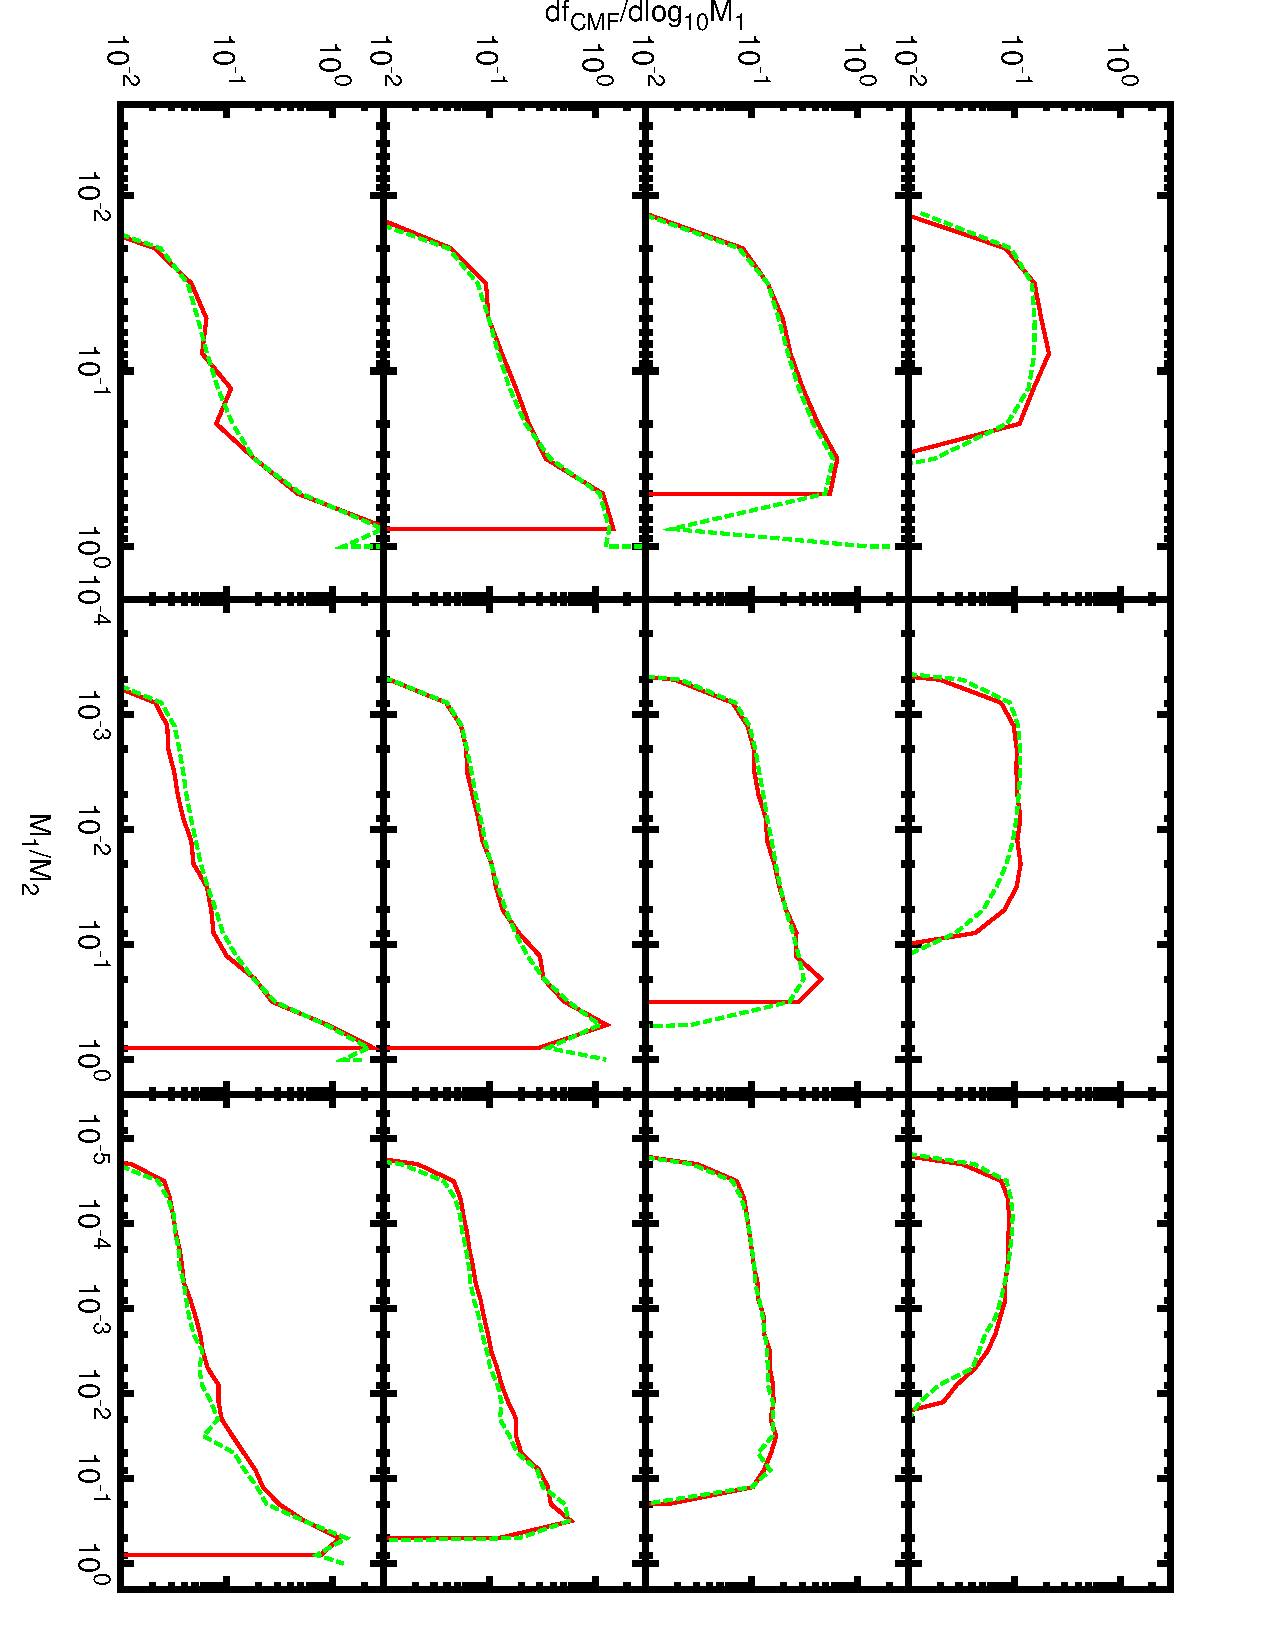
\includegraphics[height=160mm,angle=90]{../plots/progenitorMassFunction.pdf}
 \end{center}
 \caption{Progenitor mass functions at redshifts $z=0.5$, 1, 2 and 4 (bottom to top) for halos of mass $10^{12\pm0.151}$, $10^{13.5\pm0.151}$ and $10^{15\pm0.151}h^{-1}M_\odot$ (left to right) are shown. Green lines are measured from the Millennium Simulation, while red lines are computed using \glc's merger tree building routines (with the \cite{parkinson_generating_2008} branching algorithm and the \cite{cole_hierarchical_2000} tree building algorithm).}
 \label{fig:PCH_Progenitor_MFs}
\end{figure}

\subsubsection{Merger Tree Branching Modifiers}\label{sec:treeBranchingModifierMethod}

Additional methods for merger tree branching probability modifiers can be added using the {\tt treeBranchingModifierMethod} directive. The directive should contain a single argument, giving the name of a subroutine to be called to initialize the method. For example, the {\tt null} method is described by a directive:
\begin{verbatim}
 !# <treeBranchingModifierMethod>
 !#  <unitName>Merger_Tree_Branching_Modifiers_Null_Initialize</unitName>
 !# </treeBranchingModifierMethod>
\end{verbatim}
Here, {\tt Merger\_Tree\_Branching\_Modifiers\_Null\_Initialize} is the name of a subroutine which will be called to initialize the method. The initialization subroutine must have the following form:
\begin{verbatim}
 subroutine Method_Initialize(treeBranchingModifierMethod,Merger_Tree_Branching_Modifier_Get)
    type     (varying_string  ),          intent(in   ) :: treeBranchingModifierMethod
    procedure(double precision), pointer, intent(inout) :: Merger_Tree_Branching_Modifier_Get
    
    if (treeBranchingModifierMethod == 'myMethod') then
       Merger_Tree_Branching_Modifier_Get => My_Get
       .
       .
       .
    end if
    return
  end subroutine Method_Initialize
\end{verbatim}
where {\tt myMethod} is the name of this method as will be specified by the {\tt treeBranchingModifierMethod} input parameter. The procedure pointer {\tt Merger\_Tree\_Branching\_Modifier\_Get} must build and return the modifier to the branching probability as described below. The initialization subroutine should perform any other tasks required to initialize the module (such as reading parameters etc.).

The branching probability modifier function should have the interface:
\begin{verbatim}
  subroutine Merger_Tree_Branching_Modifier_Get(parentDelta,childSigma,parentSigma)
    double precision, intent(in) :: parentDelta,childSigma,parentSigma
    .
    .
    .
    return
  end subroutine Merger_Tree_Branching_Modifier_Get
\end{verbatim}
and should return the multiplicative modifier to the branching probability for the given {\tt parentDelta}, {\tt childSigma} and {\tt parentSigma}.

Currently defined merger tree branching probability modifier methods are:
\begin{description}
 \item [{\tt null}] Makes no modification;
 \item [{\tt Parkinson-Cole-Helly2008}] Modifies branching rates according to the algorithm of \cite{parkinson_generating_2008}.
\end{description}

\subsubsection{Merger Tree Building}\label{sec:MergerTreeBuildMethod}

Additional methods for merger tree building can be added using the {\tt mergerTreeBuildMethod} directive. The directive should contain a single argument, giving the name of a subroutine to be called to initialize the method. For example, the {\tt Cole2000} method is described by a directive:
\begin{verbatim}
 !# <mergerTreeBuildMethod>
 !#  <unitName>Merger_Tree_Build_Cole2000_Initialize</unitName>
 !# </mergerTreeBuildMethod>
\end{verbatim}
Here, {\tt Merger\_Tree\_Build\_Cole2000\_Initialize} is the name of a subroutine which will be called to initialize the method. The initialization subroutine must have the following form:
\begin{verbatim}
 subroutine Method_Initialize(mergerTreeBuildMethod,Merger_Tree_Build)
    type(varying_string),          intent(in)    :: mergerTreeBuildMethod
    procedure(),          pointer, intent(inout) :: Merger_Tree_Build
    
    if (mergerTreeBuildMethod == 'myMethod') then
       Merger_Tree_Build => My_Do_Tabulate
       .
       .
       .
    end if
    return
  end subroutine Method_Initialize
\end{verbatim}
where {\tt myMethod} is the name of this method as will be specified by the {\tt mergerTreeBuildMethod} input parameter. The procedure pointer {\tt Merger\_Tree\_Build} must build and return a merger tree given the a base node as described below. The initialization subroutine should perform any other tasks required to initialize the module (such as reading parameters etc.).

\begin{verbatim}
  subroutine Merger_Tree_Build_Do(thisTree)
    type(mergerTree), intent(inout) :: thisTree
    .
    .
    .
    return
  end subroutine Merger_Tree_Build_Do
\end{verbatim}
and should return a full merger tree in {\tt thisTree} built from the base node which will already be set in {\tt thisTree}. The tree must have at least masses, times and parent/child/sibling links created. Other properties (e.g. spins) can be optionally included also.

Currently defined merger tree building methods are:
\begin{description}
 \item [{\tt Cole2000}] Uses the \cite{cole_hierarchical_2000} merger tree building algorithm.
\end{description}

\subsubsection{Merger Tree Construction}\label{sec:MergerTreeConstruction}

Additional methods for merger tree construction can be added using the {\tt mergerTreeConstructMethod} directive. The directive should contain a single argument, giving the name of a subroutine to be called to initialize the method. For example, the {\tt build} method is described by a directive:
\begin{verbatim}
 !# <mergerTreeConstructMethod>
 !#  <unitName>Merger_Tree_Build_Initialize</unitName>
 !# </mergerTreeConstructMethod>
\end{verbatim}
Here, {\tt Merger\_Tree\_Build\_Initialize} is the name of a subroutine which will be called to initialize the method. The initialization subroutine must have the following form:
\begin{verbatim}
   subroutine Method_Initialize(mergerTreeConstructMethod,Merger_Tree_Construct)
    type(varying_string),          intent(in)    :: mergerTreeConstructMethod
    procedure(),          pointer, intent(inout) :: Merger_Tree_Construct
    
    if (mergerTreeConstructMethod == 'myMethod') then
       Merger_Tree_Construct => My_Do_Tabulate
       .
       .
       .
    end if
    return
  end subroutine Method_Initialize
\end{verbatim}
where {\tt myMethod} is the name of this method as will be specified by the {\tt mergerTreeConstructMethod} input parameter. The procedure pointer {\tt Merger\_Tree\_Construct} must be set to point to a function which returns a fully constructed merger tree as described below. The initialization subroutine should perform any other tasks required to initialize the module (such as reading parameters etc.).

The construction subroutine should have the following form:
\begin{verbatim}
  subroutine Merger_Tree_Construct_Do(thisTree,skipTree)
    type(mergerTree), intent(inout) :: thisTree
    logical,          intent(in)    :: skipTree
    .
    .
    .
    return
  end subroutine Merger_Tree_Construct_Do
\end{verbatim}
and should return a full merger tree in {\tt thisTree}, unless {\tt skipTree} is true, in which case this tree will be skipped (i.e. not evolved or output) and so it suffices to merely allocate the base node---there is no need to create the entire tree (although it is permissible to do so)---and update any internal data (e.g. a count of trees constructed) as required. The tree must have at least masses, times and parent/child/sibling links created. Other properties (e.g. spins) can be optionally included also. By default, the tree is assumed to be ``uninitialized'', such that the merger tree initialization function will be called prior to the tree being evolve. If the tree construction method returns a fully initialized tree it should set {\tt thisTree\%initialized=.true.}.

Currently defined merger tree construction methods are:
\begin{description}
 \item [{\tt build}] Generates a set of halo masses distributed between {\tt mergerTreeBuildHaloMassMinimum} and {\tt mergerTreeBuildHaloMassMaximum} (with {\tt mergerTreeBuildTreesPerDecade} halos per decade of mass) at redshift {\tt mergerTreeBuildTreesBaseRedshift}, or with masses read from a file, and then uses the selected merger tree build method (see \S\ref{sec:MergerTreeBuildMethod}) to build trees from these base nodes;
 \item [{\tt read}] Reads merger tree data from an HDF5 file (see \S\ref{sec:MergerTreeFiles}). The file to read is specified by the {\tt [mergerTreeReadFileName]} parameter.
 \item [{\tt smoothAccretion}] Constructs a branchless merger tree with a smooth accretion history using the selected mass accretion history method (see \S\ref{sec:HaloMassAccretionHistory}). See \S\ref{sec:SmoothAccretion} for details.
 \item [{\tt stateRestore}] Intended primarily for debugging purposes, this method will restore a tree whose complete internal state was written to file. See \S\ref{sec:TreeConstructStateRestore} for details of how to use this method.
\end{description}

\subsubsection{Non-linear Matter Power Spectrum}\index{power spectrum!non-linear}

Additional methods for the non-linear matter power spectrum can be added using the {\tt powerSpectrumNonlinearMethod} directive. The directive should contain a single argument, giving the name of a subroutine to be called to initialize the method. For example, the {\tt Peacock-Dodds1996} method is described by a directive:
\begin{verbatim}
  !# <powerSpectrumNonlinearMethod>
  !#  <unitName>Nonlinear_Power_Spectrum_Power_Law_Initialize</unitName>
  !# </powerSpectrumNonlinearMethod>
\end{verbatim}
Here, {\tt Power\_Spectrum\_Nonlinear\_PeacockDodds1996\_Initialize} is the name of a subroutine which will be called to initialize the method. The initialization subroutine must have the following form:
\begin{verbatim}
  subroutine Method_Initialize(powerSpectrumNonlinearMethod,Power_Spectrum_Nonlinear_Get)
    implicit none
    type     (varying_string  ),          intent(in   ) :: powerSpectrumNonlinearMethod
    procedure(double precision), pointer, intent(inout) :: Power_Spectrum_Nonlinear_Get
    
    if (powerSpectrumNonlinearMethod == 'myMethod') then
       Power_Spectrum_Nonlinear_Get => My_Get
       .
       .
       .
    end if
    return
  end subroutine Method_Initialize
\end{verbatim}
where {\tt myMethod} is the name of this method as will be specified by the {\tt powerSpectrumNonlinearMethod} input parameter. The procedure pointer {\tt Power\_Spectrum\_Nonlinear\_Get} must be set to point to a subroutine which computes the non-linear matter power spectrum as described below. The initialization subroutine should perform any other tasks required to initialize the module (such as reading parameters etc.).

The non-linear matter power spectrum function must have the form:
\begin{verbatim}
   double precision function Nonlinear_Power_Spectrum(wavenumber,time)
    implicit none
    double precision, intent(in   ) :: wavenumber,time
    .
    .
    .
    return
   end subroutine Nonlinear_Power_Spectrum
\end{verbatim}
The function must return the non-linear matter power spectrum, $P_{\rm nl}(k)$, at the requested {\tt wavenumber} (in units of Mpc$^{-1}$) and {\tt time} (in units of Gyr).

Currently defined non-linear matter power spectrum methods are:
\begin{description}
 \item [{\tt linear}] Simply returns the linear matter power spectrum. Intended primarily for testing purposes.
 \item [{\tt Peacock-Dodds1996}] Uses the fitting function of \cite{peacock_non-linear_1996} to compute the non-linear matter power spectrum.
 \item [{\tt CosmicEmu}] Utilizes the cosmic emulator (``CosmicEmu'') code of \cite{lawrence_coyote_2010} to compute the non-linear matter power spectrum.
\end{description}

\subsubsection{Chemical Reaction Rates}

Additional methods for chemical species reaction rates can be added using the {\tt chemicalReactionRatesMethods} directive. Note that more than one method can be specified in which cases rates are cumulative over all selected methods. The directive should contain a single argument, giving the name of a subroutine to be called to initialize the method. For example, the {\tt hydrogenNetwork} method is described by a directive:
\begin{verbatim}
  !# <chemicalReactionRatesMethods>
  !#  <unitName>Chemical_Hydrogen_Rates_Initialize</unitName>
  !# </chemicalReactionRatesMethods>
\end{verbatim}
Here, {\tt Chemical\_Hydrogen\_Rates\_Initialize} is the name of a subroutine which will be called to initialize the method. The initialization subroutine must have the following form:
\begin{verbatim}
  subroutine Method_Initialize(chemicalReactionRatesMethods)
    implicit none
    type(varying_string), intent(in) :: chemicalReactionRatesMethods
    
    if (chemicalReactionRatesMethods == 'myMethod') then
       ratesSelected = .true.
       .
       .
       .
    end if
    return
  end subroutine Method_Initialize
\end{verbatim}
where {\tt myMethod} is the name of this method as will be specified by the {\tt chemicalReactionRatesMethods} input parameter. The {\tt ratesSelected} variable is set to true if the method is active and will be checked on all subsequent calls to the module such that rates are computed only if {\tt ratesSelected} is true. The initialization subroutine should perform any other tasks required to initialize the module (such as reading parameters etc.).

The method must provide a subroutine to compute the chemical reaction rates. This subroutine is specified by the {\tt chemicalRatesCompute} directive. The directive should contain a single argument, giving the name of a subroutine to be called to compute rates. For example, the {\tt hydrogenNetwork} method uses:
\begin{verbatim}
  !# <chemicalRatesCompute>
  !#  <unitName>Chemical_Hydrogen_Rates_Compute</unitName>
  !# </chemicalRatesCompute> 
\end{verbatim}
Here, {\tt Chemical\_Hydrogen\_Rates\_Compute} is the name of a subroutine which will be called to compute the rates. The rates subroutine must have the following form:
\begin{verbatim}
  subroutine Compute_Rates(temperature,chemicalDensity,radiation,chemicalRates)
    implicit none
    type(chemicalAbundancesStructure), intent(in)    :: chemicalDensity
    double precision,                  intent(in)    :: temperature
    type(radiationStructure),          intent(in)    :: radiation
    type(chemicalAbundancesStructure), intent(inout) :: chemicalRates

    ! Exit immediately if this method is not active.
    if (.not.ratesSelected) return

    ! Compute rates for all species present.
    .
    .
    .
    return
  end subroutine Compute_Rates
\end{verbatim}
Here, {\tt temperature} is the temperature of the gas, {\tt chemicalDensity} provides the densities (in cm$^{-3}$) of all chemicals, the radiation field is described by the {\tt radiation} object and any reaction rates should be \emph{added to} the {\tt chemicalRates} object in units of cm$^{-3}$ s$^{-1}$.

Currently defined chemical reaction rate methods are:
\begin{description}
 \item [{\tt null}] A null method which does not affect any rates.
 \item [{\tt hydrogenNetwork}] Computes rates using the network of reactions and fitting functions from \cite{abel_modeling_1997} and \cite{tegmark_small_1997}.
\end{description}

\subsubsection{Population III Supernovae}

Additional methods for Population III supernovae can be added using the {\tt supernovaePopIIIMethod} directive. The directive should contain a single argument, giving the name of a subroutine to be called to initialize the method. For example, the {\tt Heger-Woosley2002} method is described by a directive:
\begin{verbatim}
  !# <supernovaePopIIIMethod>
  !#  <unitName>Supernovae_Population_III_HegerWoosley_Initialize</unitName>
  !# </supernovaePopIIIMethod>
\end{verbatim}
Here, {\tt Supernovae\_Population\_III\_HegerWoosley\_Initialize} is the name of a subroutine which will be called to initialize the method. The initialization subroutine must have the following form:
\begin{verbatim}
  subroutine Method_Initialize(supernovaePopIIIMethod,SNePopIII_Cumulative_Energy_Get)
    implicit none
    type(varying_string),          intent(in)    :: supernovaePopIIIMethod
    procedure(),          pointer, intent(inout) :: SNePopIII_Cumulative_Energy_Get
    
    if (supernovaePopIIIMethod == 'myMethod') then
       SNePopIII_Cumulative_Energy_Get => My_SNePopIII_Cumulative_Energy_Get
       .
       .
       .
    end if
    return
  end subroutine Method_Initialize
\end{verbatim}
where {\tt myMethod} is the name of this method as will be specified by the {\tt supernovaePopIIIMethod} input parameter. The procedure pointer {\tt SNePopIII\_Cumulative\_Energy\_Get} must be set to point to a function which returns the cumulative energy input from Population III supernovae as described below. The initialization subroutine should perform any other tasks required to initialize the module (such as reading parameters etc.).

The functions must have the form:
\begin{verbatim}
   double precision function PopIII_Cumulative_Energy(initialMass,age,metallicity)
    implicit none
    double precision, intent(in) :: initialMass,age,metallicity
    .
    .
    .
    return
   end function PopIII_Cumulative_Energy 
\end{verbatim}
This function must return the cumulative energy (in $M_\odot$ (km/s)$^2$) from Population III supernovae resulting from a star with given {\tt initialMass} and {\tt metallicity} after a time {\tt age}.

Currently defined population III supernovae methods are:
\begin{description}
 \item [{\tt Heger-Woosley2002}] Computes the energy input from the pair-instability results of \cite{heger_nucleosynthetic_2002}.
\end{description}

\subsubsection{Power Spectrum Variance Window Function}

Additional methods for the window function used to compute variance from the power spectrum can be added using the {\tt powerSpectrumWindowFunctionMethod} directive. The directive should contain a single argument, giving the name of a subroutine to be called to initialize the method. For example, the {\tt topHat} method is described by a directive:
\begin{verbatim}
  !# <powerSpectrumWindowFunctionMethod>
  !#  <unitName>Power_Spectrum_Window_Functions_Top_Hat_Initialize</unitName>
  !# </powerSpectrumWindowFunctionMethod>
\end{verbatim}
Here, {\tt Power\_Spectrum\_Window\_Functions\_Top\_Hat\_Initialize} is the name of a subroutine which will be called to initialize the method. The initialization subroutine must have the following form:
\begin{verbatim}
  subroutine Method_Initialize(powerSpectrumWindowFunctionMethod,Power_Spectrum_Window_Function_Get)
    implicit none
    type     (varying_string  ),          intent(in   ) :: powerSpectrumWindowFunctionMethod
    procedure(double precision), pointer, intent(inout) :: Power_Spectrum_Window_Function_Get
    
    if (powerSpectrumWindowFunctionMethod == 'myMethod') then
       Power_Spectrum_Window_Function_Get => My_Method_Do
       .
       .
       .
    end if
    return
  end subroutine Method_Initialize
\end{verbatim}
where {\tt myMethod} is the name of this method as will be specified by the {\tt powerSpectrumWindowFunctionMethod} input parameter. The procedure pointer {\tt Power\_Spectrum\_Window\_Function\_Get} must be set to point to a function which returns the window function for a given wavenumber and mass. The initialization subroutine should perform any other tasks required to initialize the module (such as reading parameters etc.).

The window function function must have the form:
\begin{verbatim}
   subroutine Power_Spectrum_Window_Function(wavenumber,smoothingMass)
    implicit none
    double precision,                            intent(in)    :: wavenumber,smoothingMass
     .
    .
    .
    return
   end subroutine Power_Spectrum_Window_Function
\end{verbatim}
The function should return the window function for the specified {\tt wavenumber} (given in Mpc$^{-1}$) and the given {\tt smoothingMass} (given in $M_\odot$).

Currently defined power spectrum variance window function methods are:
\begin{description}
 \item [{\tt topHat}] The window function is a top-hat in real-space.
 \item [{\tt kSpaceSharp}] The window function is a top-hat in $k$-space.
 \item [{\tt topHatKSpaceSharpHybrid}] A convolution of top-hat in real space and top-hat in $k$-space window functions.
\end{description}

\subsubsection{Primordial Power Spectrum}

Additional methods for the primordial power spectrum can be added using the {\tt powerSpectrumMethod} directive. The directive should contain a single argument, giving the name of a subroutine to be called to initialize the method. For example, the {\tt powerLaw} method is described by a directive:
\begin{verbatim}
  !# <powerSpectrumMethod>
  !#  <unitName>CDM_Primordial_Power_Spectrum_Power_Law_Initialize</unitName>
  !# </powerSpectrumMethod>
\end{verbatim}
Here, {\tt CDM\_Primordial\_Power\_Spectrum\_Power\_Law\_Initialize} is the name of a subroutine which will be called to initialize the method. The initialization subroutine must have the following form:
\begin{verbatim}
  subroutine Method_Initialize(powerSpectrumMethod,Power_Spectrum_Tabulate)
    implicit none
    type(varying_string),          intent(in)    :: powerSpectrumMethod
    procedure(),          pointer, intent(inout) :: Power_Spectrum_Tabulate
    
    if (powerSpectrumMethod.eq.'myMethod') then
       Power_Spectrum_Tabulate => My_Do_Tabulate
       .
       .
       .
    end if
    return
  end subroutine Method_Initialize
\end{verbatim}
where {\tt myMethod} is the name of this method as will be specified by the {\tt powerSpectrumMethod} input parameter. The procedure pointer {\tt Power\_Spectrum\_Tabulate} must be set to point to a subroutine which tabulates the power spectrum as described below. The initialization subroutine should perform any other tasks required to initialize the module (such as reading parameters etc.).

The tabulation subroutine must have the form:
\begin{verbatim}
   subroutine Power_Spectrum_Tabulate(wavenumber,powerSpectrumNumberPoints,powerSpectrumLogWavenumber,powerSpectrumLogP)
    implicit none
    double precision,                            intent(in)    :: wavenumber
    double precision, allocatable, dimension(:), intent(inout) :: powerSpectrumLogWavenumber,powerSpectrumLogP
    integer,                                     intent(out)   :: powerSpectrumNumberPoints
    .
    .
    .
    return
   end subroutine Power_Spectrum_Tabulate
\end{verbatim}
The subroutine must tabulate the natural log of the power spectrum in array {\tt powerSpectrumLogP()} as a function of the natural log of wavenumber {\tt powerSpectrumLogWavenumber()} (these arrays must be allocated to the correct size, and may be prevously allocated, therefore requiring a deallocation). The number of tabulated points should be returned in {\tt powerSpectrumNumberPoints}. The subroutine should ensure that the currently requested {\tt wavenumber} is within the range of the tabulated function (preferably with some buffer).

Currently defined power spectrum methods are:
\begin{description}
 \item [{\tt powerLaw}] The power spectrum is assumed to be a power law, possibly with a running index. It is defined by
\begin{equation}
 P(k)\propto k^{n_{\rm s} + \ln(k/k_{\rm ref}) [\d n /\d\ln k]},
\end{equation}
where the parameters are specified by input parameters $n_{\rm s}\equiv${\tt powerSpectrumIndex}, $k_{\rm ref}\equiv${\tt powerSpectrumReferenceWavenumber} and $\d n / \d \ln k \equiv${\tt powerSpectrumRunning}.
\end{description}

\subsubsection{Radiation Components}\index{radiation}\label{sec:radiationComponents}

Radiation components (i.e. types of radiation field that may be added to any radiation object; see \S\ref{sec:RadiationSubsystem}) are defined using a combination of several directives: {\tt radiationLabel}, {\tt radiationSet}, {\tt radiationTemperature} and {\tt radiationFlux}. For example, the cosmic microwave background radiation component is defined by the following set of directives:
\begin{verbatim}
  !# <radiationLabel>
  !#  <label>CMB</label>
  !# </radiationLabel>

  !# <radiationSet>
  !#  <unitName>Radiation_Set_CMB</unitName>
  !#  <label>CMB</label>
  !# </radiationSet>

  !# <radiationTemperature>
  !#  <unitName>Radiation_Temperature_CMB</unitName>
  !#  <label>CMB</label>
  !# </radiationTemperature>

  !# <radiationFlux>
  !#  <unitName>Radiation_Flux_CMB</unitName>
  !#  <label>CMB</label>
  !# </radiationFlux>
\end{verbatim}
The first of these, {\tt radiationLabel}, should contain a single element, {\tt label}, which gives a label that will be used to identify this component, both in other directives and also in the internal parameters used to select this radiation component (e.g. in this case, a parameter {\tt radiationTypeCMB} will be available within \glc\ to select the cosmic microwave background component). The other directives must all specify the same {\tt label} element and additional give, in a {\tt unitName} element, the name of a function/subroutine to be called to perform the relevant calculation.

The {\tt radiationSet} directive must specify a subroutine with the following template:
\begin{verbatim}
  subroutine Radiation_Set(componentMatched,thisNode,radiationProperties)
   implicit none
   logical,          intent(in)                               :: componentMatched
   type(treeNode),   intent(inout), pointer                   :: thisNode
   double precision, intent(inout), allocatable, dimension(:) :: radiationProperties

   if (.not.componentMatched) return
   .
   .
   .
   return
  end subroutine Radiation_Set
\end{verbatim}
If {\tt componentMatched} is true, then the subroutine should set the radiation component, otherwise it should exit immediately. If the radiation component is to be set, then the routine can allocate the {\tt radiationProperties} array as necessary to store any data needed to specify the radiation field. These data should then be set using, if necessary, any relevant information from {\tt thisNode}.

The {\tt radiationTemperature} directive should specify a subroutine with the following template:
\begin{verbatim}
  subroutine Radiation_Temperature(requestedType,ourType,radiationProperties,radiationTemperature,radiationType)
   implicit none
   integer,          intent(in)                            :: requestedType,ourType
   double precision, intent(in),              dimension(:) :: radiationProperties
   double precision, intent(inout)                         :: radiationTemperature
   integer,          intent(in),    optional, dimension(:) :: radiationType

   if (requestedType /= ourType) return
   if (present(radiationType)) then
      if (all(radiationType /= ourType)) return
   end if
   .
   .
   .
   return
  end subroutine Radiation_Temperature
\end{verbatim}
The tests in the above should always be included so that the subroutine exits immediately if the component type is not active or not requested. Once these tests have been made, the subroutine should set the temperature (in units of Kelvin) of the radiation field (if applicable).

The {\tt radiationFlux} directive should specify a subroutine with the following template:
\begin{verbatim}
  subroutine Radiation_Flux(requestedType,ourType,radiationProperties,wavelength,radiationFlux,radiationType)
    implicit none
    integer,          intent(in)                           :: requestedType,ourType
    double precision, intent(in)                           :: wavelength
    double precision, intent(in),             dimension(:) :: radiationProperties
    double precision, intent(inout)                        :: radiationFlux
    integer,          intent(in),   optional, dimension(:) :: radiationType

    if (requestedType /= ourType) return
    if (present(radiationType)) then
       if (all(radiationType /= ourType)) return
    end if
    .
    .
    .
    return
  end subroutine Radiation_Flux
\end{verbatim}
The tests in the above should always be included so that the subroutine exits immediately if the component type is not active or not requested. Once these tests have been made, the subroutine should add the flux (in units of ergs cm$^2$ s$^{-1}$ Hz$^{-1}$ ster$^{-1}$) at the specified {\tt wavelength} (in units of \AA) of the radiation field to that in {\tt radiationFlux}.

Currently defined radiation component types are:
\begin{description}
 \item [{\tt null}] A null component with no radiation.
 \item [{\tt CMB}] The cosmic microwave background, assumed to be a perfect blackbody spectrum with a temperature equal to {\tt [T\_CMB]}$(1+z)$.
 \item [{\tt IGB}] The intergalactic background light, set using the method selected by {\tt [radiationIntergalacticBackgroundMethod]; see \S\ref{sec:radiationIGB}}.
\end{description}

\subsubsection{Radiation Components: Intergalactic Background}\label{sec:radiationIGB}

Additional methods for the intergalactic background radiation component can be added using the {\tt radiationIntergalacticBackgroundMethod} directive. The directive should contain a single argument, giving the name of a subroutine to be called to initialize the method. For example, the {\tt file} method is described by a directive:
\begin{verbatim}
 !# <radiationIntergalacticBackgroundMethod>
 !#  <unitName>Radiation_IGB_File_Initialize</unitName>
 !# </radiationIntergalacticBackgroundMethod>
\end{verbatim}
Here, {\tt Radiation\_IGB\_File\_Initialize} is the name of a subroutine which will be called to initialize the method. The initialization subroutine must have the following form:
\begin{verbatim}
  subroutine Method_Initialize(radiationIntergalacticBackgroundMethod,Radiation_Set_Intergalactic_Background_Do,Radiation_Flux_Intergalactic_Background_Do)
    implicit none
    type(varying_string),          intent(in)    :: radiationIntergalacticBackgroundMethod
    procedure(),          pointer, intent(inout) :: Radiation_Set_Intergalactic_Background_Do,Radiation_Flux_Intergalactic_Background_Do
    
    if (radiationIntergalacticBackgroundMethod == 'myMethod') then
      Radiation_Set_Intergalactic_Background_Do  => My_Method_Set
      Radiation_Flux_Intergalactic_Background_Do => My_Method_Flux
    end if
    return
  end subroutine Method_Initialize
\end{verbatim}
where {\tt myMethod} is the name of this method as will be specified by the {\tt radiationIntergalacticBackgroundMethod} input parameter. The procedure pointers {\tt Radiation\_Set\_Intergalactic\_Background\_Do} and {\tt Radiation\_Flux\_Intergalactic\_Background\_Do} must be set to point to subroutines which set the radiation field and return its flux as described below. The initialization subroutine should perform any other tasks required to initialize the module (such as reading parameters etc.).

The set subroutine must have the form:
\begin{verbatim}
  subroutine My_Method_Set(thisNode,radiationProperties)
    implicit none
    type(treeNode),   intent(inout), pointer                   :: thisNode
    double precision, intent(inout), allocatable, dimension(:) :: radiationProperties

    return
  end subroutine My_Method_Set
\end{verbatim}
and should set the radiation component as described in \S\ref{sec:radiationComponents}. The flux subroutine must have the form:
\begin{verbatim}
   subroutine My_Method_Flux(radiationProperties,wavelength,radiationFlux)
    implicit none
    double precision, intent(in)                 :: wavelength
    double precision, intent(in),   dimension(:) :: radiationProperties
    double precision, intent(inout)              :: radiationFlux

    return
   end subroutine My_Method_Flux
\end{verbatim}
and should increment {\tt radiationFlux} as described in \S\ref{sec:radiationComponents}.

Currently defined intergalactic background radiation methods are:
\begin{description}
 \item [{\tt file}] The intergalatic background radiation field, specified as a function of cosmic time, is read from a file. The flux is determined by linearly interpolating to the required time and wavelength. The XML file to read is specified by {\tt [radiationIGBFileName]}. An example of the required file structure is:
 \begin{verbatim}
<spectrum>
  <URL>http://adsabs.harvard.edu/abs/1996ApJ...461...20H</URL>
  <description>Cosmic background radiation spectrum from quasars alone.</description>
  <reference>Haardt, F. &amp; Madau, P. 1996, ApJ, 461, 20</reference>
  <source>Francesco Haardt on Aug 6 2005, via Cloudy 08.00</source>
  <wavelengths>
    <datum>0.0002481</datum>
    <datum>0.001489</datum>
    .
    .
    .
    <units>Angstroms</units>
  </wavelengths>
  <spectra>
    <datum>7.039E-49</datum>
    <datum>8.379E-48</datum>
    <datum>1.875E-39</datum>
    <datum>7.583E-38</datum>
    .
    .
    .
    <redshift>0</redshift>
    <units>erg cm^-2 s^-1 Hz^-1 sr^-1</units>
  </spectra>
</spectrum>
 \end{verbatim}
\end{description}
The optional {\tt URL}, {\tt description}, {\tt reference} and {\tt source} elements can be used to give the provenance of the data. The {\tt wavelengths} element should contain a set of {\tt datum} elements each containing a wavelength (in increasing order) at which the spectrum will be tabulated. Wavelengths must be given in Angstroms. Multiple {\tt spectra} elements can be given, each specifying the spectrum at a redshift as given in the {\tt redshift} element. Each {\tt spectra} element must contain an array of {\tt datum} elements that gives the spectrum at each wavelength listed in the {\tt wavelength} element. Spectra must be in units of erg cm$^{-2}$ s$^{-1}$ Hz$^{-1}$ sr$^{-1}$.

\subsubsection{Satellite Merging Mass Movements}

Additional methods for the satellite merging mass movements can be added using the {\tt satelliteMergingMassMovementsMethod} directive. The directive should contain a single argument, giving the name of a subroutine to be called to initialize the method. For example, the {\tt simple} method is described by a directive:
\begin{verbatim}
 !# <satelliteMergingMassMovementsMethod>
 !#  <unitName>Satellite_Merging_Mass_Movements_Simple_Initialize</unitName>
 !# </satelliteMergingMassMovementsMethod>
\end{verbatim}
Here, {\tt Satellite\_Merging\_Mass\_Movements\_Simple\_Initialize} is the name of a subroutine which will be called to initialize the method. The initialization subroutine must have the following form:
\begin{verbatim}
  subroutine Method_Initialize(satelliteMergingMassMovementsMethod,Satellite_Merging_Mass_Movement_Get)
    implicit none
    type(varying_string),          intent(in)    :: satelliteMergingMassMovementsMethod
    procedure(),          pointer, intent(inout) :: Satellite_Merging_Mass_Movement_Get
    
    if (satelliteMergingMassMovementsMethod == 'simple') Satellite_Merging_Mass_Movement_Get => My_Method_Get
    return
  end subroutine Method_Initialize
\end{verbatim}
where {\tt myMethod} is the name of this method as will be specified by the {\tt satelliteMergingMassMovementsMethod} input parameter. The procedure pointer {\tt Satellite\_Merging\_Mass\_Movement\_Get} must be set to point to a function which sets the mass movement descriptors as described below. The initialization subroutine should perform any other tasks required to initialize the module (such as reading parameters etc.).

The mass movement subroutine must have the form:
\begin{verbatim}
  subroutine My_Method_Get(thisNode,gasMovesTo,starsMoveTo,hostGasMovesTo,hostStarsMoveTo,mergerIsMajor)
    implicit none
    type(treeNode), intent(inout), pointer  :: thisNode
    integer,        intent(out)             :: gasMovesTo,starsMoveTo,hostGasMovesTo,hostStarsMoveTo
    logical,        intent(out)             :: mergerIsMajor
    .
    .
    .
    return
  end subroutine My_Method_Get
\end{verbatim}
The subroutine must return values for each of the ``{\tt MoveTo}'' descriptors to specify where stars and gas from {\tt thisNode} and {\tt thisNode}'s host node should move to in the host. Allowed values are:
\begin{description}
 \item [{\tt movesToDisk}] The material in question moves to the disk of the host node;
 \item [{\tt movesToSpheroid}] The material in question moves to the spheroid of the host node;
 \item [{\tt doesNotMove}] The material in question does not move (allowed only for host node descriptors).
\end{description}
Additionally, the {\tt mergerIsMajor} flag should be set to indicate whether this merger is deemed to be ``major'' (typically defined as one which redistributes mass from a disk into a spheroidal component).

Currently defined satellite merger mass movement methods are:
\begin{description}
 \item [{\tt verySimple}] In this case, the satellite is always added to the disk of the host, while material in the host does not move.
 \item [{\tt simple}] If the baryonic mass of the satellite exceeds a fraction {\tt majorMergerMassRatio} of the baryonic mass of the host then all material is moved to the spheroid of the host. Otherwise, satellite gas moves to the component given by {\tt minorMergerGasMovesTo}, satellite stars move to the host spheroid and host material does not move.
 \item [{\tt Baugh2005}] If the baryonic mass of the satellite exceeds a fraction {\tt majorMergerMassRatio} of the baryonic mass of the host then all material is moved to the spheroid of the host. Otherwise, if the baryonic mass of the satellite exceeds a fraction {\tt burstMassRatio} of the baryonic mass of the host and the gas fraction in the host exceeds {\tt burstCriticalGasFraction} then all gas is moved to the host spheroid, while the host stellar disk remains in place. For mergers failing both criteria, satellite gas moves to the component given by {\tt minorMergerGasMovesTo}, satellite stars move to the host spheroid and host material does not move. 
\end{description}

\subsubsection{Satellite Merging Remnant Sizes}\label{sec:satelliteMergerMassMovementMethod}

Additional methods for the satellite merging remnant sizes can be added using the {\tt satelliteMergingRemnantSizeMethod} directive. The directive should contain a single argument, giving the name of a subroutine to be called to initialize the method. For example, the {\tt Cole2000} method is described by a directive:
\begin{verbatim}
 !# <satelliteMergingRemnantSizeMethod>
 !#  <unitName>Satellite_Merging_Remnant_Sizes_Cole2000_Initialize</unitName>
 !# </satelliteMergingRemnantSizeMethod>
\end{verbatim}
Here, {\tt Satellite\_Merging\_Remnant\_Sizes\_Cole2000\_Initialize} is the name of a subroutine which will be called to initialize the method. The initialization subroutine must have the following form:
\begin{verbatim}
  subroutine Method_Initialize(satelliteMergingRemnantSizeMethod,Satellite_Merging_Remnant_Size_Do)
    implicit none
    type(varying_string),          intent(in)    :: satelliteMergingRemnantSizeMethod
    procedure(),          pointer, intent(inout) :: Satellite_Merging_Remnant_Size_Do
    
    if (satelliteMergingRemnantSizeMethod == 'myMethod') Satellite_Merging_Remnant_Size_Do => My_Method_Do
    return
  end subroutine Method_Initialize
\end{verbatim}
where {\tt myMethod} is the name of this method as will be specified by the {\tt satelliteMergingRemnantSizeMethod} input parameter. The procedure pointer {\tt Satellite\_Merging\_Remnant\_Size\_Do} must be set to point to a function which computes the size of the merger remnant and stores the properties (e.g. radius, circular velocity and specific angular momentum at the half-mass radius) of the \emph{host} node. The initialization subroutine should perform any other tasks required to initialize the module (such as reading parameters etc.).

The remnant size subroutine must have the form:
\begin{verbatim}
  subroutine My_Method_Do(thisNode)
    implicit none
    type(treeNode), intent(inout), pointer  :: thisNode
    .
    .
    .
    return
  end subroutine My_Method_Do
\end{verbatim}
The subroutine must compute the properties of the merger remnant. Typically these are stored in the {\tt Satellite\_Merging\_Remnant\_Sizes\_Properties} module for later retrieval by the appropriate component.

Currently defined satellite merger remnant size methods are:
\begin{description}
 \item [{\tt null}] This is a null method which does nothing. It is useful for runs where no baryonic components are included (e.g. for studying dark matter only).
 \item [{\tt Cole2000}] Implements the algorithm of \cite{cole_hierarchical_2000} to compute the remnant size. The orbital energy assumed can be adjusted using the {\tt mergerRemnantSizeOrbitalEnergy} parameter, which is equivalent to the $f_{\rm orbit}$ parameter of \cite{cole_hierarchical_2000}.
 \item [{\tt Covington2008}] Implements the algorithm of \cite{covington_predicting_2008} to compute the remnant size. The orbital energy assumed can be adjusted using the {\tt mergerRemnantSizeOrbitalEnergy} parameter, which is equivalent to the $f_{\rm orbit}$ parameter of \cite{cole_hierarchical_2000}.
\end{description}

\subsubsection{Satellite Merging Remnants: Progenitor Properties}

Additional methods for satellite merging remnant progenitor properties can be added using the {\tt satelliteMergingRemnantProgenitorPropertiesMethod} directive. The directive should contain a single argument, giving the name of a subroutine to be called to initialize the method. For example, the {\tt standard} method is described by a directive:
\begin{verbatim}
 !# <satelliteMergingRemnantProgenitorPropertiesMethod>
 !#  <unitName>Satellite_Merging_Remnant_Progenitor_Properties_Standard_Init</unitName>
 !# </satelliteMergingRemnantProgenitorPropertiesMethod>
\end{verbatim}
Here, {\tt Satellite\_Merging\_Remnant\_Progenitor\_Properties\_Standard\_Init} is the name of a subroutine which will be called to initialize the method. The initialization subroutine must have the following form:
\begin{verbatim}
  subroutine Method_Initialize(satelliteMergingRemnantProgenitorPropertiesMethod,Satellite_Merging_Remnant_Progenitor_Properties_Get)
    implicit none
    type(varying_string),          intent(in)    :: satelliteMergingRemnantProgenitorPropertiesMethod
    procedure(),          pointer, intent(inout) :: Satellite_Merging_Remnant_Progenitor_Properties_Get
    
    if (satelliteMergingRemnantProgenitorPropertiesMethod == 'myMethod') Satellite_Merging_Remnant_Progenitor_Properties_Get => My_Method_Get
    return
  end subroutine Method_Initialize
\end{verbatim}
where {\tt myMethod} is the name of this method as will be specified by the {\tt satelliteMergingRemnantProgenitorPropertiesMethod} input parameter. The procedure pointer {\tt Satellite\_Merging\_Remnant\_Progenitor\_Properties\_Get} must be set to point to a subroutine which computes various properties of the progenitor galaxies involved in the merger, as described below. The initialization subroutine should perform any other tasks required to initialize the module (such as reading parameters etc.).

The progenitor properties subroutine must have the form:
\begin{verbatim}
  subroutine My_Method_Get(satelliteNode,hostNode,satelliteMass,hostMass,satelliteSpheroidMass &
       & ,hostSpheroidMass,hostSpheroidMassPreMerger,satelliteRadius,hostRadius &
       & ,angularMomentumFactor,remnantSpheroidMass,remnantSpheroidGasMass)
    implicit none
    type(treeNode),   intent(inout), pointer :: satelliteNode,hostNode
    double precision, intent(out)            :: satelliteMass,hostMass,satelliteSpheroidMass, &
       & hostSpheroidMass,hostSpheroidMassPreMerger,satelliteRadius,hostRadius, &
       & angularMomentumFactor,remnantSpheroidMass,remnantSpheroidGasMass
    .
    .
    .
    return
  end subroutine My_Method_Do
\end{verbatim}
The subroutine must compute properties of the merger progenitor galaxies in {\tt satelliteNode} and {\tt hostNode}: {\tt satelliteMass} and {\tt hostMass} are the total masses of the two galaxies; {\tt satelliteSpheroidMass} and {\tt hostSpheroidMass} are the masses of each galaxy that will end up in the spheroid of the merger remnant; {\tt hostSpheroidMassPreMerger} is the mass of the host spheroid prior to the merger; {\tt satelliteRadius} and {\tt hostRadius} are radii of the two galaxies for use in merger remnant size calculations (and so should typically refer to the radius of material that will end up in the merger remnant spheroid); {\tt remnantSpheroidMass} is the mass of the spheroid in the remnant; {\tt remnantSpheroidGasMass} is the mass of gas in the spheroid of the remnant; and {\tt angularMomentumFactor} gives the pseudo-specific angular momentum of the remnant in units of $({\rm G} M_{\rm remnant,spheroid} r_{\rm remnant,spheroid})^{1/2}$ where $M_{\rm remnant,spheroid}$ is the mass of the 
remnant spheroid and $r_{\rm remnant,spheroid}$ is the radius of the remnant spheroid.

Currently defined satellite merger progenitor properties methods are:
\begin{description}
 \item [{\tt Cole2000}] Implements the algorithm of \cite{cole_hierarchical_2000} to compute the remnant properties. Masses of host and spheroid are set equal to their stellar plus cold gas masses utilizing, while radii are the half-mass radii of each galaxy, including only those components which end up in the remnant spheroid. The angular momentum factor is set to a mass-weighted average of the corresponding factor for each component which will end up in the merger remnant spheroid.
 \item [{\tt standard}] Masses of host and spheroid are set equal to their stellar plus cold gas masses utilizing, while radii are a mass-weighted average of the half-mass radii of the components which end up in the merger remnant spheroid. The angular momentum factor is similarly set to a mass-weighted average of the corresponding factor for each component which will end up in the merger remnant spheroid.
\end{description}

\subsubsection{Satellite Merging Timescales}

Additional methods for the satellite merging timescales can be added using the {\tt satelliteMergingMethod} directive. The directive should contain a single argument, giving the name of a subroutine to be called to initialize the method. For example, the {\tt Lacey-Cole} method is described by a directive:
\begin{verbatim}
  !# <satelliteMergingMethod>
  !#  <unitName>Satellite_Time_Until_Merging_Lacey_Cole_Initialize</unitName>
  !# </satelliteMergingMethod>
\end{verbatim}
Here, {\tt Satellite\_Time\_Until\_Merging\_Lacey\_Cole\_Initialize} is the name of a subroutine which will be called to initialize the method. The initialization subroutine must have the following form:
\begin{verbatim}
  subroutine Method_Initialize(satelliteMergingMethod,Satellite_Time_Until_Merging)
    implicit none
    type(varying_string),          intent(in)    :: satelliteMergingMethod
    procedure(),          pointer, intent(inout) :: Satellite_Time_Until_Merging
    
    if (satelliteMergingMethod == 'myMethod') Satellite_Time_Until_Merging => My_Method_Procedure
    return
  end subroutine Method_Initialize
\end{verbatim}
where {\tt myMethod} is the name of this method as will be specified by the {\tt satelliteMergingMethod} input parameter. The procedure pointer {\tt Satellite\_Time\_Until\_Merging} must be set to point to a function which returns the time until merging as described below. The initialization subroutine should perform any other tasks required to initialize the module (such as reading parameters etc.).

The merging timescale function must have the form:
\begin{verbatim}
 double precision function Satellite_Time_Until_Merging(thisNode,thisOrbit)
    implicit none
    type(treeNode),    pointer, intent(inout) :: thisNode
    type(keplerOrbit),          intent(inout) :: thisOrbit
    .
    .
    .
    return
 end function Satellite_Time_Until_Merging
\end{verbatim}
The function must return the merging timescale for {\tt thisNode} orbitting with {\tt thisOrbit} at virial radius crossing in {\tt thisNode\%parentNode} in units of Gyr.

Currently defined satellite virial orbit methods are:
\begin{description}
 \item [\hyperlink{satellites.merging.dynamical_friction.timescale.Lacey-Cole.F90:dynamical_friction_lacey_cole:satellite_time_until_merging_lacey_cole}{{\tt Lacey-Cole}}] Computes the merging timescale using the method of \cite{lacey_merger_1993}.
 \item [\hyperlink{satellites.merging.dynamical_friction.timescale.Lacey-Cole_Tormen.F90:dynamical_friction_lacey_cole_tormen:satellite_time_until_merging_lacey_cole_tormen}{{\tt Lacey-Cole+Tormen}}] Computes the merging timescale using the method of \cite{lacey_merger_1993} with a parameterization of orbital parameters designed to fit the results of \cite{tormen_rise_1997} as described by \cite{cole_hierarchical_2000};
 \item [\hyperlink{satellites.merging.dynamical_friction.timescale.Jiang2008.F90:dynamical_friction_jiang2008:satellite_time_until_merging_jiang2008}{{\tt Jiang2008}}] Computes the merging timescale using the method of \cite{jiang_fitting_2008};
 \item [\hyperlink{satellites.merging.dynamical_friction.timescale.Boylan-Kolchin2008.F90:dynamical_friction_boylankolchin2008:satellite_time_until_merging_boylankolchin2008}{{\tt BoylanKolchin2008}}] Computes the merging timescale using the method of \cite{boylan-kolchin_dynamical_2008};
 \item [\hyperlink{satellites.merging.preset.F90:satellite_merging_times_preset:satellite_time_until_merging_preset}{{\tt preset}}] This method assumes that merging times have been preset for every node (or, at least, every node which becomes a satellite). It therefore simply returns the preset merging time;
 \item [\hyperlink{satellites.merging.dynamical_friction.timescale.Wetzel-White.F90:dynamical_friction_wetzel_white:satellite_time_until_merging_wetzel_white}{{\tt Wetzel-White}}] Computes the merging timescale using the method of \cite{wetzel_what_2010}.
\end{description}

\subsubsection{Satellite Virial Orbits}\label{sec:SatelliteVirialOrbits}

Additional methods for the satellite virial orbits (i.e. orbital parameters at virial radius crossing) can be added using the {\tt virialOrbitsMethod} directive. The directive should contain a single argument, giving the name of a subroutine to be called to initialize the method. For example, the {\tt Benson2005} method is described by a directive:
\begin{verbatim}
  !# <virialOrbitsMethod>
  !#  <unitName>Virial_Orbital_Parameters_Benson2005_Initialize</unitName>
  !# </virialOrbitsMethod>
\end{verbatim}
Here, {\tt Virial\_Orbital\_Parameters\_Benson2005\_Initialize} is the name of a subroutine which will be called to initialize the method. The initialization subroutine must have the following form:
\begin{verbatim}
  subroutine Method_Initialize(virialOrbitsMethod,Virial_Orbital_Parameters_Get)
    implicit none
    type(varying_string),          intent(in)    :: virialOrbitsMethod
    procedure(),          pointer, intent(inout) :: Virial_Orbital_Parameters_Get
    
    if (virialOrbitsMethod.eq.'myMethod') Virial_Orbital_Parameters_Get => My_Method_Procedure
    return
  end subroutine Method_Initialize
\end{verbatim}
where {\tt myMethod} is the name of this method as will be specified by the {\tt virialOrbitsMethod} input parameter. The procedure pointer {\tt Virial\_Orbital\_Parameters\_Get} must be set to point to a subroutine which returns orbital parameters as described below. The initialization subroutine should perform any other tasks required to initialize the module (such as reading parameters etc.).

The orbital parameter subroutine must have the form:
\begin{verbatim}
  function Virial_Orbital_Parameters(thisNode,hostNode,acceptUnboundOrbits) result (thisOrbit)
    implicit none
    type(keplerOrbit)                         :: thisOrbit
    type(treeNode),   intent(inout), pointer  :: thisNode,hostNode
    logical,          intent(in)              :: acceptUnboundOrbits
    .
    .
    .
    return
  end subroutine Virial_Orbital_Parameters
\end{verbatim}
The subroutine must return a fully-defined Kepler orbit object (i.e. the orbit must have at least three parameters defined in addition to the node masses) initialized to the orbital parameters for {\tt thisNode} orbitting in {\tt hostNode} at the point of virial radius crossing. If {\tt acceptUnboundOrbits} is true, then unbound orbits may be returned, otherwise, the routine must ensure that the returned orbit is bound. Velocities should be returned in units of km/s, lengthscales in units of Mpc and masses in $M_\odot$. Note that the usual conventions of the {\tt keplerOrbit} object should be followed, namely the that orbitting bodies are treated as point masses, with the host being stationary and the usual reduced mass used.

Currently defined satellite virial orbit methods are:
\begin{description}
 \item [\hyperlink{satellites.merging.virial_orbits.Benson2005.F90:virial_orbits_benson2005:virial_orbital_parameters_benson2005}{{\tt Benson2005}}] The orbital parameters are select from the distribution found by \cite{benson_orbital_2005}.
 \item [\hyperlink{satellites.merging.virial_orbits.Wetzel2010.F90:virial_orbits_wetzel2010:virial_orbital_parameters_wetzel2010}{{\tt Wetzel2010}}] The orbital parameters are select from the distribution found by \cite{wetzel_orbits_2010}.
 \item [\hyperlink{satellites.merging.virial_orbits.fixed.F90:virial_orbits_fixed:virial_orbital_parameters_fixed}{{\tt fixed}}] The orbital parameters are set to fixed values, with $v_{\rm r}=${\tt [virialOrbitsFixedRadialVelocity]}$V_{\rm virial}$ and  $v_\phi=${\tt [virialOrbitsFixedTangentialVelocity]}$V_{\rm virial}$.
\end{description}

\subsubsection{Star Formation Feedback in Disks/Spheroids}

Additional methods for computing feedback from star formation in disks/spheroids can be added using the {\tt starFormationFeedback[Disks|Spheroids]Method} directive. The directive should contain a single argument, giving the name of a subroutine to be called to initialize the method. For example, the {\tt powerLaw} method is described by a directive:
\begin{verbatim}
 !# <starFormationFeedbackSpheroidsMethod>
 !#  <unitName>Star_Formation_Feedback_Spheroids_Power_Law_Initialize</unitName>
 !# </starFormationFeedbackSpheroidsMethod>
\end{verbatim}
Here, {\tt Star\_Formation\_Feedback\_Spheroids\_Power\_Law\_Initialize} is the name of a subroutine which will be called to initialize the method. The initialization subroutine must have the following form:
\begin{verbatim}
  subroutine Method_Initialize(starFormationFeedbackDisksMethod,Star_Formation_Feedback_Disk_Outflow_Rate_Get)
    implicit none
    type(varying_string),          intent(in)    :: starFormationFeedbackDisksMethod
    procedure(),          pointer, intent(inout) :: Star_Formation_Feedback_Disk_Outflow_Rate_Get
    
    if (starFormationFeedbackDisksMethod == 'myMethod') Star_Formation_Feedback_Disk_Outflow_Rate_Get => My_Star_Formation_Feedback_Disk_Outflow_Rate_Get
    return
  end subroutine Method_Initialize
\end{verbatim}
where {\tt myMethod} is the name of this method as will be specified by the {\tt starFormationFeedback[Disks|Spheroids]Method} input parameter. The procedure pointer {\tt Star\_Formation\_Feedback\_Disk\_Outflow\_Rate\_Get} (or {\tt Star\_Formation\_Feedback\_Spheroid\_Outflow\_Rate\_Get} for the spheroid case) must be set to point to a function which returns the mass outflow rate due to star formation as described below. The initialization subroutine should perform any other tasks required to initialize the module (such as reading parameters etc.).

The outflow rate function must have the form:
\begin{verbatim}
 double precision function Star_Formation_Feedback_Outflow_Rate_Get(thisNode,starFormationRate,energyInputRate)
    implicit none
    type(treeNode),   intent(inout), pointer :: thisNode
    double precision, intent(in)             :: starFormationRate,energyInputRate
    .
    .
    .
    return
 end function Star_Formation_Feedback_Outflow_Rate_Get
\end{verbatim}
The function must return the mass outflow rate (in $M_\odot$ Gyr$^{-1}$) for {\tt thisNode}.

Currently defined star formation feedback methods are:
\begin{description}
 \item [\hyperlink{star_formation.feedback.disks.fixed.F90:star_formation_feedback_disks_fixed}{{\tt fixed}}] The outflow rate is a fixed multiple of the the star formation rate.
 \item [\hyperlink{star_formation.feedback.spheroids.power_law.F90:star_formation_feedback_spheroids_power_law:star_formation_feedback_spheroid_outflow_rate_power_law}{{\tt powerLaw}}] The outflow rate is given by
\begin{equation}
 \dot{M}_{\rm outflow} = \left({V_{\rm outflow} \over V}\right)^{\alpha_{\rm outflow}} {\dot{E} \over E_{\rm canonical}},
\end{equation}
where $V_{\rm outflow}=${\tt [disk|spheroid]OutflowVelocity} (in km/s) and $\alpha_{\rm outflow}=${\tt [disk|spheroid]OutflowVelocity} are input parameters, $V$ is the characteristic velocity of the component, $\dot{E}$ is the rate of energy input from stellar populations and $E_{\rm canonical}$ is the total energy input by a canonical stellar population normalized to $1 M_\odot$ after infinite time.
 \item [\hyperlink{star_formation.feedback.disks.Creasy2012.F90:star_formation_feedback_disks_creasy2012}{{\tt Creasey2012}}] The outflow rate computed using the model of \cite{creasey_how_2012}.
\end{description}

\subsubsection{(Expulsive) Star Formation Feedback in Disks/Spheroids}\index{feedback!expulsive}

Additional methods for computing expulsive feedback\footnote{``Expulsive'' feedback implies outflows in which gas is driven not only out of a galaxy but also out of its host dark matter halo.} from star formation in disks/spheroids can be added using the {\tt starFormationExpulsiveFeedback[Disks|Spheroids]Method} directive. The directive should contain a single argument, giving the name of a subroutine to be called to initialize the method. For example, the {\tt powerLaw} method is described by a directive:
\begin{verbatim}
 !# <starFormationExpulsiveFeedbackSpheroidsMethod>
 !#  <unitName>Star_Formation_Expulsive_Feedback_Spheroids_Power_Law_Initialize</unitName>
 !# </starFormationExpulsiveFeedbackSpheroidsMethod>
\end{verbatim}
Here, {\tt Star\_Formation\_Expulsive\_Feedback\_Spheroids\_Power\_Law\_Initialize} is the name of a subroutine which will be called to initialize the method. The initialization subroutine must have the following form:
\begin{verbatim}
  subroutine Method_Initialize(starFormationExpulsiveFeedbackDisksMethod,Star_Formation_Expulsive_Feedback_Disk_Outflow_Rate_Get)
    implicit none
    type(varying_string),          intent(in)    :: starFormationFeedbackDisksMethod
    procedure(),          pointer, intent(inout) :: Star_Formation_Expulsive_Feedback_Disk_Outflow_Rate_Get
    
    if (starFormationExpulsiveFeedbackDisksMethod == 'myMethod') Star_Formation_Expulsive_Feedback_Disk_Outflow_Rate_Get => My_Star_Formation_Expulsive_Feedback_Disk_Outflow_Rate_Get
    return
  end subroutine Method_Initialize
\end{verbatim}
where {\tt myMethod} is the name of this method as will be specified by the {\tt starFormationExpulsiveFeedback[Disks|Spheroids]Method} input parameter. The procedure pointer {\tt Star\_Formation\_Expulsive\_Feedback\_Disk\_Outflow\_Rate\_Get} (or {\tt Star\_Formation\_Expulsive\_Feedback\_Spheroid\_Outflow\_Rate\_Get} for the spheroid case) must be set to point to a function which returns the expulsive mass outflow rate due to star formation as described below. The initialization subroutine should perform any other tasks required to initialize the module (such as reading parameters etc.).

The outflow rate function must have the form:
\begin{verbatim}
 double precision function Star_Formation_Expulsive_Feedback_Outflow_Rate_Get(thisNode,starFormationRate,energyInputRate)
    implicit none
    type(treeNode),   intent(inout), pointer :: thisNode
    double precision, intent(in)             :: starFormationRate,energyInputRate
    .
    .
    .
    return
 end function Star_Formation_Expulsive_Feedback_Outflow_Rate_Get
\end{verbatim}
The function must return the expulsive mass outflow rate (in $M_\odot$ Gyr$^{-1}$) for {\tt thisNode}.

Currently defined star formation expulsive feedback methods are:
\begin{description}
 \item [\hyperlink{star_formation.feedback_expulsion.spheroids.null.F90:star_formation_expulsive_feedback_spheroids_null:star_formation_expulsive_feedback_spheroid_outflow_rate_null}{{\tt null}}] Assumes a zero outflow rate.
 \item [\hyperlink{star_formation.feedback_expulsion.spheroids.superwind.F90:star_formation_expulsive_feedback_spheroids_superwind:star_formation_expulsive_feedback_spheroid_outflow_rate_sw}{{\tt superwind}}] The outflow rate is given by
\begin{equation}
 \dot{M}_{\rm outflow} = \beta_{\rm superwind} {\dot{E} \over E_{\rm canonical}} \left\{ \begin{array}{ll} \left( V_{\rm superwind}/V\right)^2 & \hbox{ if } V > V_{\rm superwind} \\ 1 & \hbox{ otherwise,} \end{array} \right.
\end{equation}
where $V_{\rm superwind}=${\tt [disk|spheroid]SuperwindVelocity} (in km/s) and $\beta_{\rm superwind}=${\tt [disk|spheroid]SuperwindMassLoading} are input parameters, $V$ is the characteristic velocity of the component, $\dot{E}$ is the rate of energy input from stellar populations and $E_{\rm canonical}$ is the total energy input by a canonical stellar population normalized to $1 M_\odot$ after infinite time.
\end{description}

\subsubsection{Star Formation Rate Surface Density in Disks}

Additional methods for computing the surface density of star formation rate in disks can be added using the {\tt starFormationRateSurfaceDensityDisksMethod} directive. The directive should contain a single argument, giving the name of a subroutine to be called to initialize the method. For example, the {\tt Blitz-Rosolowsky2006} method is described by a directive:
\begin{verbatim}
 !# <starFormationRateSurfaceDensityDisksMethod>
 !#  <unitName>Star_Formation_Rate_Surface_Density_Disks_BR_Initialize</unitName>
 !# </starFormationRateSurfaceDensityDisksMethod>
\end{verbatim}
Here, {\tt Star\_Formation\_Rate\_Surface\_Density\_Disks\_BR\_Initialize} is the name of a subroutine which will be called to initialize the method. The initialization subroutine must have the following form:
\begin{verbatim}
  subroutine Method_Initialize(starFormationRateSurfaceDensityDisksMethod,Star_Formation_Rate_Surface_Density_Disk_Get)
    implicit none
    type(varying_string),          intent(in)    :: starFormationRateSurfaceDensityDisksMethod
    procedure(),          pointer, intent(inout) :: Star_Formation_Rate_Surface_Density_Disk_Get
    
    if (starFormationRateSurfaceDensityDisksMethod == 'myMethod') Star_Formation_Rate_Surface_Density_Disk_Get => My_Method_Get
    return
  end subroutine Method_Initialize
\end{verbatim}
where {\tt myMethod} is the name of this method as will be specified by the {\tt starFormationRateSurfaceDensityDisksMethod} input parameter. The procedure pointer {\tt Star\_Formation\_Rate\_Surface\_Density\_Disk\_Get} must be set to point to a function which returns the surface density of star formation rate at a specified radius as described below. The initialization subroutine should perform any other tasks required to initialize the module (such as reading parameters etc.).

The star formation rate surface density function must have the form:
\begin{verbatim}
 double precision function Star_Formation_Rate_Surface_Density_Get(thisNode,radius)
    implicit none
    type            (treeNode), intent(inout), pointer :: thisNode
    double precision          , intent(in   )          :: radius
    .
    .
    .
    return
 end function Star_Formation_Rate_Surface_Density_Get
\end{verbatim}
The function must return the surface density of star formation rate (in units of $M_\odot$ Gyr$^{-1}$ Mpc$^{-2}$) for {\tt thisNode}.

Currently defined star formation rate surface density methods are:
\begin{description}
 \item [\hyperlink{star_formation.rate_surface_density.disks.Kennicutt-Schmidt.F90:star_formation_rate_surface_density_disks_ks:star_formation_rate_surface_density_disk_ks}{{\tt Kennicutt-Schmidt}}] The rate is given by the Kennicutt-Schmidt law (\citealt{schmidt_rate_1959,kennicutt_global_1998}; see \S\ref{sec:StarFormationKennicuttSchmidt}).
 \item [\hyperlink{star_formation.rate_surface_density.disks.extended_Schmidt.F90:star_formation_rate_surface_density_disks_exschmidt:star_formation_rate_surface_density_disk_exschmidt}{{\tt extendedSchmidt}}] The rate is given by the extended Schmidt law (\citealt{shi_extended_2011}; see \S\ref{sec:StarFormationExtendedSchmidt}).
 \item [\hyperlink{star_formation.rate_surface_density.disks.Blitz-Rosolowsky.F90:star_formation_rate_surface_density_disks_br:star_formation_rate_surface_density_disk_br}{{\tt Blitz-Rosolowsky2006}}] The rate is given by the Blitz-Rosolowsky rule (\citealt{blitz_role_2006}; see \S\ref{sec:StarFormationBlitzRosolowsky}).
 \item [\hyperlink{star_formation.rate_surface_density.disks.KMT09.F90:star_formation_rate_surface_density_disks_kmt09:star_formation_rate_surface_density_disk_kmt09}{{\tt KMT09}}] The rate is given by the Krumholz-McKee-Tumlinson (\citealt{krumholz_star_2009}; see \S\ref{sec:StarFormationKMT09});
\end{description}

\subsubsection{Star Formation Timescale in Disks/Spheroids}

Additional methods for computing star formation timescales in disks/spheroids can be added using the {\tt starFormationTimescale[Disks|Spheroids]Method} directive. The directive should contain a single argument, giving the name of a subroutine to be called to initialize the method. For example, the {\tt dynamicalTime} method is described by a directive:
\begin{verbatim}
 !# <starFormationTimescaleDisksMethod>
 !#  <unitName>Star_Formation_Timescale_Disks_Dynamical_Time_Initialize</unitName>
 !# </starFormationTimescaleDisksMethod>
\end{verbatim}
Here, {\tt Star\_Formation\_Timescale\_Disks\_Dynamical\_Time\_Initialize} is the name of a subroutine which will be called to initialize the method. The initialization subroutine must have the following form:
\begin{verbatim}
  subroutine Method_Initialize(starFormationTimescaleDisksMethod,Star_Formation_Timescale_Disk_Get)
    implicit none
    type(varying_string),          intent(in)    :: starFormationTimescaleDisksMethod
    procedure(),          pointer, intent(inout) :: Star_Formation_Timescale_Disk_Get
    
    if (starFormationTimescaleDisksMethod == 'myMethod') Star_Formation_Timescale_Disk_Get => My_Method_Get_Procedure
    return
  end subroutine Method_Initialize
\end{verbatim}
where {\tt myMethod} is the name of this method as will be specified by the {\tt starFormationTimescale[Disks|Spheroids]Method} input parameter. The procedure pointer {\tt Star\_Formation\_Timescale\_Disk\_Get} (or {\tt Star\_Formation\_Timescale\_Spheroid\_Get} for the spheroid case) must be set to point to a function which returns the timescale for star formation as described below. The initialization subroutine should perform any other tasks required to initialize the module (such as reading parameters etc.).

The star formation timescale function must have the form:
\begin{verbatim}
 double precision function Star_Formation_Timescale_Get(thisNode)
    implicit none
    type(treeNode), intent(in) :: thisNode
    .
    .
    .
    return
 end function Star_Formation_Timescale_Get
\end{verbatim}
The function must return the star formation timescale (in units of Gyr) for {\tt thisNode}.

Currently defined star formation timescale methods are:
\begin{description}
 \item [\hyperlink{star_formation.timescales.disks.halo_scaling.F90:star_formation_timescale_disks_halo_scaling}{{\tt haloScaling}}]  The timescale scales with halo virial velocity and redshift;
 \item [\hyperlink{star_formation.timescales.disks.fixed.F90:star_formation_timescale_disks_fixed}{{\tt fixed}}]  The timescale is a fixed quantity;
 \item [\hyperlink{star_formation.timescales.disks.dynamical_time.F90:star_formation_timescale_disks_dynamical_time:star_formation_timescale_disk_dynamical_time}{{\tt dynamicalTime}}]  The timescale is given by
\begin{equation}
 \tau_\star = \epsilon_\star^{-1} \tau_{\rm dynamical, [disk|spheroid]} \left( {V_{\rm [disk|spheroid]} \over 200\hbox{km/s}} \right)^{\alpha_\star},
\end{equation}
where $\epsilon_\star$(={\tt starFormation[Disk|Spheroid]Efficiency}) is a star formation efficiency and $\alpha_\star$(={\tt starFormation[Disk|Spheroid]VelocityExponent}) controls the scaling with velocity. Note that $\tau_{\rm dynamical,[disk|spheroid]}=R_{\rm [disk|spheroid]}/V_{\rm [disk|spheroid]}$ where the radius and velocity are whatever characteristic values returned by the disk/spheroid method. This scaling is functionally similar to that adopted by \cite{cole_hierarchical_2000}, but they specifically used the half-mass radius and circular velocity at that radius.
 \item {\tt Baugh2005}] The timescale is given by $\tau_0 (V_{\rm disk}/200\hbox{km/s})^\alpha a^\beta$.
 \item {\tt integratedSurfaceDensity}] The timescale is given by $\tau_\star = M_{\rm cold}/\int_0^\infty 2 \pi r \dot{\Sigma}_\star(r) {\rm d}r$ where $\dot{\Sigma}_\star(r)$ is the surface density of star formation rate (see \S\ref{sec:StarFormationRateSurfaceDensity})
\end{description}

\subsubsection{Stellar Astrophysics}

Additional methods for stellar astrophysical properties can be added using the {\tt stellarAstrophysicsMethod} directive. The directive should contain a single argument, giving the name of a subroutine to be called to initialize the method. For example, the {\tt file} method is described by a directive:
\begin{verbatim}
  !# <stellarAstrophysicsMethod>
  !#  <unitName>Stellar_Astrophysics_File_Initialize</unitName>
  !# </stellarAstrophysicsMethod>
\end{verbatim}
Here, {\tt Stellar\_Astrophysics\_File\_Initialize} is the name of a subroutine which will be called to initialize the method. The initialization subroutine must have the following form:
\begin{verbatim}
  subroutine Method_Initialize(stellarAstrophysicsMethod,Star_Ejected_Mass_Get,Star_Initial_Mass_Get,Star_Metal_Yield_Mass_Get,Star_Lifetime_Get)
    implicit none
    type(varying_string),          intent(in)    :: stellarAstrophysicsMethod
    procedure(),          pointer, intent(inout) :: Star_Ejected_Mass_Get,Star_Initial_Mass_Get,Star_Metal_Yield_Mass_Get,Star_Lifetime_Get
    
    if (stellarAstrophysicsMethod == 'myMethod') then
      Star_Ejected_Mass_Get     => My_Star_Ejected_Mass
      Star_Initial_Mass_Get     => My_Star_Initial_Mass
      Star_Metal_Yield_Mass_Get => My_Star_Metal_Yield_Mass
      Star_Lifetime_Get         => My_Star_Lifetime
    end if
    return
  end subroutine Method_Initialize
\end{verbatim}
where {\tt myMethod} is the name of this method as will be specified by the {\tt stellarAstrophysicsMethod} input parameter. The procedure pointers must be set to point to functions which return stellar properties as described below. The initialization subroutine should perform any other tasks required to initialize the module (such as reading parameters etc.).

The ejected mass and lifetime functions must have the form:
\begin{verbatim}
 double precision function Star_Property(initialMass,metallicity)
    implicit none
    double precision, intent(in) :: initialMass,metallicity
    .
    .
    .
    return
 end function Star_Property
\end{verbatim}
These functions must return the total ejected mass (in $M_\odot$), total metal yield (in $M_\odot$) and lifetime (in Gyr) for a star of the specified {\tt initialMass} and {\tt metallicity}.

The metal yield function must have the form:
\begin{verbatim}
 double precision function Star_Metal_Yield(initialMass,metallicity,atomIndex)
    implicit none
    double precision, intent(in)           :: initialMass,metallicity
    integer,          intent(in), optional :: atomIndex
    .
    .
    .
    return
 end function Star_Property
\end{verbatim}
This function must return the yield (in $M_\odot$) of the element identified by {\tt atomIndex} (as returned by the \hyperlink{atomic.data.F90:atomic_data:atom_lookup}{{\tt Atom\_Lookup()}} function from the \hyperlink{atomic.data.F90:atomic_data}{{\tt Atomic\_Data}} module) if present, or total metal yield otherwise for a star of the specified {\tt initialMass} and {\tt metallicity}.

The initial mass function must have the form:
\begin{verbatim}
 double precision function Star_Initial_Mass(lifetime,metallicity)
    implicit none
    double precision, intent(in) :: lifetime,metallicity
    .
    .
    .
    return
 end function Star_Initial_Mass
\end{verbatim}
and should return the initial mass (in $M_\odot$) of a star of given {\tt lifetime} (specified in Gyr) and {\tt metallicity}.

Currently defined stellar astrophysics methods are:
\begin{description}
 \item [{\tt file}] Stellar properties are read from an XML file and interpolated. The structure of the XML file is described in \S\ref{sec:StellarAstrophysicsFile}.
\end{description}

\subsubsection{Stellar Population Properties}

Additional methods for computing properties of stellar populations can be added using the {\tt stellarPopulationPropertiesMethod} directive. The directive should contain a single argument, giving the name of a subroutine to be called to initialize the method. For example, the {\tt instantaneous} method is described by a directive:
\begin{verbatim}
 !# <stellarPopulationPropertiesMethod>
 !#  <unitName>Stellar_Population_Properties_Instantaneous_Initialize</unitName>
 !# </stellarPopulationPropertiesMethod>
\end{verbatim}
Here, {\tt Stellar\_Population\_Properties\_Instantaneous\_Initialize} is the name of a subroutine which will be called to initialize the method. The initialization subroutine must have the following form:
\begin{verbatim}
  subroutine Method_Initialize(stellarPopulationPropertiesMethod,Stellar_Population_Properties_Rates_Get &
 & ,Stellar_Population_Properties_Scales_Get,Stellar_Population_Properties_History_Count_Get             &
 & ,Stellar_Population_Properties_History_Create_Do)
    implicit none
    type(varying_string),          intent(in)    :: stellarPopulationPropertiesMethod
    procedure(),          pointer, intent(inout) :: Stellar_Population_Properties_Rates_Get  &
 & ,Stellar_Population_Properties_Scales_Get,Stellar_Population_Properties_History_Count_Get &
 & ,Stellar_Population_Properties_History_Create_Do
    
    if (stellarPopulationPropertiesMethod == 'myMethod') then
       Stellar_Population_Properties_Rates_Get         => My_Method_Rates_Get_Procedure
       Stellar_Population_Properties_Scales_Get        => My_Method_Scales_Procedure
       Stellar_Population_Properties_History_Count_Get => My_Method_History_Count_Get_Procedure
       Stellar_Population_Properties_History_Create_Do => My_Method_History_Create_Procedure
    end if
    return
  end subroutine Method_Initialize
\end{verbatim}
where {\tt myMethod} is the name of this method as will be specified by the {\tt stellarPopulationPropertiesMethod} input parameter. The procedure pointers {\tt Stellar\_Population\_Properties\_Rates\_Get} and {\tt Stellar\_Population\_Properties\_Scales\_Get} must be set to point to subroutines which return properties of a stellar population and set scaling factors for ODE error control as described below, while the {\tt Stellar\_Population\_Properties\_History\_Count\_Get} and {\tt Stellar\_Population\_Properties\_History\_Create\_Do} procedure pointers must be set to point to functions which return the number of histories that will be required by this method and create a suitable history object respectively. The initialization subroutine should perform any other tasks required to initialize the module (such as reading parameters etc.).

The stellar populations properties subroutine must have the form:
\begin{verbatim}
 subroutine Stellar_Population_Properties_Rates(starFormationRate,fuelAbundances,component,thisNode,thisHistory,stellarMassRate&
       &,stellarAbundancesRates,stellarLuminositiesRates,fuelMassRate,fuelAbundancesRates,energyInputRate)
    implicit none
    implicit none
    double precision,          intent(out)                 :: stellarMassRate,fuelMassRate,energyInputRate
    type(abundancesStructure), intent(out)                 :: stellarAbundancesRates,fuelAbundancesRates
    integer,                   intent(in)                  :: component
    double precision,          intent(out),   dimension(:) :: stellarLuminositiesRates
    double precision,          intent(in)                  :: starFormationRate
    type(abundancesStructure), intent(in)                  :: fuelAbundances
    type(treeNode),            intent(inout), pointer      :: thisNode
    type(history),             intent(inout)               :: thisHistory
    .
    .
    .
    return
 end subroutine Stellar_Population_Properties_Rates
\end{verbatim}
The subroutine is given the {\tt starFormationRate} (in $M_\odot$ Gyr$^{-1}$) in {\tt thisNode}. Any history information required by this method must be passed in via the {\tt history} argument. Stars are forming from fuel material with composition specified by {\tt fuelAbundances} and occurring in the specified galactic {\tt component} (using the labels provided by the \hyperlink{galactic_structure.options.F90:galactic_structure_options}{{\tt Galactic\_Structure\_Options}} module). The subroutine must return the rates of change of stellar and fuel mass (in $M_\odot$ Gyr$^{-1}$) in {\tt stellarMassRate} and {\tt fuelMassRate} respectively, and the corresponding rates (also in $M_\odot$ Gyr$^{-1}$) of abundance change in {\tt stellarAbundancesRates} and {\tt fuelAbundancesRates} respectively. Finally, it should return rates of change (in $L_{\rm AB}$ Gyr$^{-1}$) of stellar luminosities for all requested output bands in {\tt stellarLuminositiesRates}. Additionally, the rate of energy input from stellar 
populations must be returned in {\tt energyInputRate}.

The scales procedure should have the form:
\begin{verbatim}
  subroutine Stellar_Population_Properties_Scales_Noninstantaneous(thisHistory,stellarMass,stellarAbundances)
   implicit none
   double precision,          intent(in)    :: stellarMass
   type(abundancesStructure), intent(in)    :: stellarAbundances
   type(history),             intent(inout) :: thisHistory
   .
   .
   .
   return
 end subroutine Stellar_Population_Properties_Scales_Noninstantaneous
\end{verbatim}
and should set scale factors for ODE error control (see \S\ref{sec:ComponentEvolution}) in the stellar population properties history {\tt thisHistory}. The {\tt stellarMass} and {\tt stellarAbundances} (both in $M_\odot$) are provided as input as they are often useful in choosing appropriate scale factors.

The history count function must have the form
\begin{verbatim}
 integer function Stellar_Population_Properties_History_Count()
    implicit none
    .
    .
    return
 end function Stellar_Population_Properties_History_Count
\end{verbatim}
and should return the number of histories that will be required by this method. The history create function must have the form
\begin{verbatim}
  subroutine Stellar_Population_Properties_History_Create(thisNode,thisHistory)
   type(treeNode),  intent(inout), pointer :: thisNode
   type(history),   intent(inout)          :: thisHistory
   .
   .
   .
   return
 end subroutine Stellar_Population_Properties_History_Create
\end{verbatim}
and should create {\tt thisHistory} with a suitable set of time steps for {\tt thisNode}.

Currently defined stellar population properties methods are:
\begin{description}
 \item [\hyperlink{stellar_populations.properties.instantaneous.F90:stellar_population_properties_instantaneous:stellar_population_properties_rates_instantaneous}{{\tt instantaneous}}] Computes stellar population properties using an instantaneous recyclying approximation.
\end{description}

\subsubsection{Stellar Population Spectra}\label{sec:StellarPopulationSpectra}

Additional methods for computing specta of stellar populations can be added using the {\tt stellarPopulationSpectraMethod} directive. The directive should contain a single argument, giving the name of a subroutine to be called to initialize the method. For example, the {\tt Conroy-White-Gunn2009} method is described by a directive:
\begin{verbatim}
 !# <stellarPopulationSpectraMethod>
 !#  <unitName>Stellar_Population_Spectra_Conroy_Initialize</unitName>
 !# </stellarPopulationSpectraMethod>
\end{verbatim}
Here, {\tt Stellar\_Population\_Spectra\_Conroy\_Initialize} is the name of a subroutine which will be called to initialize the method. The initialization subroutine must have the following form:
\begin{verbatim}
  subroutine Method_Initialize(stellarPopulationSpectraMethod,Stellar_Population_Spectra_Get,Stellar_Population_Spectrum_Tabulation_Get)
    implicit none
    type(varying_string),          intent(in)    :: stellarPopulationSpectraMethod
    procedure(),          pointer, intent(inout) :: Stellar_Population_Spectra_Get,Stellar_Population_Spectrum_Tabulation_Get
    
    if (stellarPopulationSpectraMethod == 'myMethod') then
        Stellar_Population_Spectra_Get             => My_Method_Spectra_Get
        Stellar_Population_Spectrum_Tabulation_Get => My_Method_Spectrum_Tabulation_Get
    end if
    return
  end subroutine Method_Initialize
\end{verbatim}
where {\tt myMethod} is the name of this method as will be specified by the {\tt stellarPopulationSpectraMethod} input parameter. The procedure pointer {\tt Stellar\_Population\_Spectra\_Get} must be set to point to a function which returns the spectrum of a stellar population as described below while the {\tt Stellar\_Population\_Spectrum\_Tabulation\_Get} pointer must be set to point to a subroutine which returns a tabulation of ages and metallicities on which stellar spectra should be tabulated. The initialization subroutine should perform any other tasks required to initialize the module (such as reading parameters etc.).

The stellar spectra function must have the form:
\begin{verbatim}
  double precision function Stellar_Population_Spectra_Get(abundances,age,wavelength,imfIndex)
    implicit none
    type(abundancesStructure), intent(in) :: abundances
    double precision,          intent(in) :: age,wavelength
    integer,                   intent(in) :: imfIndex
    .
    .
    .
    return
  end function Stellar_Population_Spectra_Get
\end{verbatim}
The function is given the {\tt abundances}, {\tt age} (in Gyr), and {\tt imfIndex} of the stellar population and the {\tt wavelength} (in \AA) at which the spectrum should be computed. The spectrum should be returned in units of $L_\odot$ Hz$^{-1}$.

The tabulation subroutine must have the form:
\begin{verbatim}
  subroutine Stellar_Population_Spectrum_Tabulation(imfIndex,agesCount,metallicitiesCount,age,metallicity)
    implicit none
    integer,          intent(in)                             :: imfIndex
    integer,          intent(out)                            :: agesCount,metallicitiesCount
    double precision, intent(out), allocatable, dimension(:) :: age,metallicity
    .
    .
    .
    return
  end subroutine Stellar_Population_Spectrum_Tabulation
\end{verbatim}
and should return the number of ages and metallicities at which stellar population spectra should be tabualted for the specified \gls{imf}, and should allocate the {\tt age} and {\tt metallicity} arrays appropriately and should fill them with the ages and metallicities at which to tabulate.

Currently defined stellar population properties methods are:
\begin{description}
 \item [\hyperlink{stellar_populations.spectra.Conroy_et_al.F90:stellar_population_spectra_conroy}{{\tt Conroy-White-Gunn2009}}] Uses the {\tt FSPS} code of \cite{conroy_propagation_2009} to compute stellar spectra. If necessary, the {\tt FSPS} code will be downloaded, patched and compiled and run to generate spectra. These tabulations are then stored to file for later retrieval.
 \item [\hyperlink{stellar_populations.spectra.file.F90:stellar_population_spectra_file}{{\tt file}}] Stellar spectra for a given \gls{imf} are read from the file specified by the {\tt stellarPopulationSpectraForXXXXIMF} where {\tt XXXX} is the name of the \gls{imf}. This should specify an HDF5 file with the following structure:
\begin{verbatim}
 ages                     Dataset {ageCount}
 metallicities            Dataset {metallicityCount}
 spectra                  Dataset {metallicityCount, ageCount, metallicityCount}
 wavelengths              Dataset {wavelengthCount}
\end{verbatim}
where the datasets contain the tabulated ages (in Gyr), metallicities (logarithmic, relative to Solar), wavelengths (in \AA) and spectra (in $L_\odot$ Hz$^{-1}$).
\end{description}
Currently, the following pre-computed stellar spectra files are available as a separate download from \href{http://users.obs.carnegiescience.edu/abenson/galacticus/data/Galacticus_SSP_Data.tar.bz2}{\tt http://users.obs.carnegiescience.edu/abenson/galacticus/data/Galacticus\_SSP\_Data.tar.bz2}:
\begin{description}
 \item [{\tt data/SSP\_Spectra\_Conroy-et-al\_v2.0\_imfSalpeter.hdf5}] Corresponds to a Salpeter IMF computed using v2.0 of the {\tt FSPS} code;
 \item [{\tt data/SSP\_Spectra\_Conroy-et-al\_v2.1\_imfSalpeter.hdf5}]  Corresponds to a Salpeter IMF computed using v2.1 of the {\tt FSPS} code;
 \item [{\tt data/SSP\_Spectra\_Conroy-et-al\_v2.1\_imfChabrier.hdf5}]  Corresponds to a Chabrier IMF computed using v2.1 of the {\tt FSPS} code;
 \item [{\tt data/SSP\_Spectra\_Conroy-et-al\_v2.2\_imfChabrier.hdf5}]  Corresponds to a Chabrier IMF computed using v2.2 of the {\tt FSPS} code;
 \item [{\tt data/SSP\_Spectra\_Conroy-et-al\_v2.2\_imfKennicutt.hdf5}]  Corresponds to a Kennicutt IMF computed using v2.2 of the {\tt FSPS} code;
 \item [{\tt data/SSP\_Spectra\_Conroy-et-al\_v2.2\_imfBaugh2005TopHeavy.hdf5}]  Corresponds to the top-heavy IMF of \cite{baugh_can_2005} computed using v2.2 of the {\tt FSPS} code;
 \item [{\tt data/SSP\_Spectra\_Maraston\_hbMorphologyRed\_imfKroupa.hdf5}] The spectra from \cite{maraston_evolutionary_2005} for a Kroupa IMF and a red horizontal branch morphology;
 \item [{\tt data/SSP\_Spectra\_Maraston\_hbMorphologyRed\_imfSalpeter.hdf5}] The spectra from \cite{maraston_evolutionary_2005} for a Salpeter IMF and a red horizontal branch morphology; 
 \item [{\tt data/SSP\_Spectra\_BC2003\_highResolution\_imfChabrier.hdf5}] The (high resolution) spectra from \cite{bruzual_stellar_2003} for a Chabrier IMF, using Padova 1994 tracks;
 \item [{\tt data/SSP\_Spectra\_BC2003\_highResolution\_imfSalpeter.hdf5}] The (high resolution) spectra from \cite{bruzual_stellar_2003} for a Salpeter IMF, using Padova 1994 tracks;
 \item [{\tt data/SSP\_Spectra\_BC2003\_lowResolution\_imfChabrier.hdf5}] The (low resolution) spectra from \cite{bruzual_stellar_2003} for a Chabrier IMF, using Padova 1994 tracks;
 \item [{\tt data/SSP\_Spectra\_BC2003\_lowResolution\_imfSalpeter.hdf5}] The (low resolution) spectra from \cite{bruzual_stellar_2003} for a Salpeter IMF, using Padova 1994 tracks;
 \item [{\tt data/SSP\_Spectra\_Grasil\_gkn15rd\_ken.hdf5}] The spectra used by {\sc Grasil} for a Kennicutt IMF;
 \item [{\tt data/SSP\_Spectra\_Grasil\_gkn1rd\_ken.hdf5}] The spectra used by {\sc Grasil} for a Kennicutt IMF;
 \item [{\tt data/SSP\_Spectra\_Grasil\_gsrdk0b\_sal.hdf5}] The spectra used by {\sc Grasil} for a Salpeter IMF;
 \item [{\tt data/SSP\_Spectra\_Grasil\_imf27\_kro.hdf5}] Spectra used by {\sc Grasil}.
\end{description}
Note that the high resolution spectra from \cite{bruzual_stellar_2003} may require you to adjust the {\tt [stellarPopulationLuminosityIntegrationToleranceRelative]} parameter to a larger value. The sharp features in these high resolution spectra can be difficult to integrate. Scripts to convert the data provided by \cite{maraston_evolutionary_2005} and \cite{bruzual_stellar_2003} into \glc's format are provided in the {\tt scripts/ssps} folder. Spectra for other initial mass functions will be computed automatically when using the \cite{conroy_propagation_2009} population synthesis models.

\subsubsection{Stellar Population Spectra Postprocessing}

Additional methods for postprocessing specta of stellar populations can be added using the {\tt stellarPopulationSpectraPostprocessMethod} directive. The directive should contain a single argument, giving the name of a subroutine to be called to initialize the method. For example, the {\tt Meiksin2006} method is described by a directive:
\begin{verbatim}
 !# <stellarPopulationSpectraPostprocessMethod>
 !#  <unitName>Stellar_Population_Spectra_Postprocess_Meiksin2006_Initialize</unitName>
 !# </stellarPopulationSpectraPostprocessMethod>
\end{verbatim}
Here, {\tt Stellar\_Population\_Spectra\_Postprocess\_Meiksin2006\_Initialize} is the name of a subroutine which will be called to initialize the method. The initialization subroutine must have the following form:
\begin{verbatim}
  subroutine Method_Initialize(stellarPopulationSpectraPostprocessMethod,Stellar_Population_Spectra_Postprocess_Get)
    implicit none
    type(varying_string),          intent(in)    :: stellarPopulationSpectraPostprocessMethod
    procedure(),          pointer, intent(inout) :: Stellar_Population_Spectra_Postprocess_Get
    
    if (stellarPopulationSpectraPostprocessMethod == 'myMethod') then
        Stellar_Population_Spectra_Postprocess_Get => My_Method_Postprocess_Get
    end if
    return
  end subroutine Method_Initialize
\end{verbatim}
where {\tt myMethod} is the name of this method as will be specified by the {\tt stellarPopulationSpectraPostprocessMethod} input parameter. The procedure pointer {\tt Stellar\_Population\_Spectra\_Postprocess\_Get} must be set to point to a function which returns a multiplicative factor by which stellar spectra will be scaled. The initialization subroutine should perform any other tasks required to initialize the module (such as reading parameters etc.).

The stellar spectra postprocessing function must have the form:
\begin{verbatim}
  double precision function Stellar_Population_Spectra_Postprocess_Get(wavelength,redshift)
    implicit none
    double precision, intent(in) :: wavelength,redshift
    .
    .
    .
    return
  end function Stellar_Population_Spectra_Postprocess_Get
\end{verbatim}
The function is given the rest-frame {\tt wavelength} (in \AA) and the {\tt redshift} of the radiation and should return a multiplicative factor by which the spectrum will be scaled.

Currently defined stellar population postprocessing methods are:
\begin{description}
\item [\hyperlink{stellar_populations.spectra.postprocess.Meiksin2006.F90:stellar_population_spectra_postprocessing_meiksin2006}{{\tt Meiksin2006}}] Postprocesses spectra through absorption by the \gls{igm} using the results of \cite{meiksin_colour_2006}.
\item [\hyperlink{stellar_populations.spectra.postprocess.Madau1995.F90:stellar_population_spectra_postprocessing_madau1995}{{\tt Madau1995}}] Postprocesses spectra through absorption by the \gls{igm} using the results of \cite{madau_radiative_1995}.
\item [\hyperlink{stellar_populations.spectra.postprocess.null.F90:stellar_population_spectra_postprocess_null}{{\tt null}}] Performs no postprocessing.
\end{description}

\subsubsection{Stellar Feedback}

Additional methods for stellar feedback can be added using the {\tt stellarFeedbackMethod} directive. The directive should contain a single argument, giving the name of a subroutine to be called to initialize the method. For example, the {\tt standard} method is described by a directive:
\begin{verbatim}
  !# <stellarFeedbackMethod>
  !#  <unitName>Stellar_Feedback_Standard_Initialize</unitName>
  !# </stellarFeedbackMethod>
\end{verbatim}
Here, {\tt Stellar\_Feedback\_Standard\_Initialize} is the name of a subroutine which will be called to initialize the method. The initialization subroutine must have the following form:
\begin{verbatim}
  subroutine Method_Initialize(stellarFeedbackMethod,Stellar_Feedback_Cumulative_Energy_Input_Get)
    implicit none
    type(varying_string),          intent(in)    :: stellarFeedbackMethod
    procedure(),          pointer, intent(inout) :: Stellar_Feedback_Cumulative_Energy_Input_Get
    
    if (stellarFeedbackMethod == 'myMethod') then
       Stellar_Feedback_Cumulative_Energy_Input_Get => My_Stellar_Feedback_Cumulative_Energy_Input_Get
       .
       .
       .
    end if
    return
  end subroutine Method_Initialize
\end{verbatim}
where {\tt myMethod} is the name of this method as will be specified by the {\tt stellarFeedbackMethod} input parameter. The procedure pointer {\tt Stellar\_Feedback\_Cumulative\_Energy\_Input\_Get} must be set to point to a function which returns the cumulative energy input from stars as described below. The initialization subroutine should perform any other tasks required to initialize the module (such as reading parameters etc.).

The function must have the form:
\begin{verbatim}
   double precision function Stellar_Feedback_Cumulative_Energy_Input(initialMass,age,metallicity)
    implicit none
    double precision, intent(in) :: initialMass,age,metallicity
    .
    .
    .
    return
   end function Stellar_Feedback_Cumulative_Energy_Input 
\end{verbatim}
The function must return the cumulative energy input (in $M_\odot$ (km/s)$^2$ from stars of given {\tt initialMass} and {\tt metallicity} after a time {\tt age}.

Currently defined stellar feedback methods are:
\begin{description}
 \item [{\tt standard}] This method assumes that the energy input has contributions from stellar winds, Type Ia, Type II and Population III supernovae. The minimum mass required for a star to produce a Type II supernova is specified via {\tt initialMassForSupernovaeTypeII} (in $M_\odot$), while the energy per Type II or Ia supernova is specified via {\tt supernovaEnergy} (in ergs).
\end{description}

\subsubsection{Stellar Tracks}

Additional methods for stellar tracks can be added using the {\tt stellarTracksMethod} directive. The directive should contain a single argument, giving the name of a subroutine to be called to initialize the method. For example, the {\tt file} method is described by a directive:
\begin{verbatim}
  !# <stellarTracksMethod>
  !#  <unitName>Stellar_Tracks_Initialize_File</unitName>
  !# </stellarTracksMethod>
\end{verbatim}
Here, {\tt Stellar\_Tracks\_Initialize\_File} is the name of a subroutine which will be called to initialize the method. The initialization subroutine must have the following form:
\begin{verbatim}
  subroutine Method_Initialize(stellarTracksMethod,Stellar_Luminosity_Get,Stellar_Effective_Temperature_Get)
    implicit none
    type(varying_string),          intent(in)    :: stellarTracksMethod
    procedure(),          pointer, intent(inout) :: Stellar_Luminosity_Get,Stellar_Effective_Temperature_Get
    
    if (stellarTracksMethod == 'myMethod') then
       Stellar_Luminosity_Get            => My_Stellar_Luminosity_Get
       Stellar_Effective_Temperature_Get => My_Stellar_Effective_Temperature_Get
       .
       .
       .
    end if
    return
  end subroutine Method_Initialize
\end{verbatim}
where {\tt myMethod} is the name of this method as will be specified by the {\tt stellarTracksMethod} input parameter. The procedure pointers {\tt Stellar\_Luminosity\_Get} and {\tt Stellar\_Effective\_Temperature\_Get} must be set to point to functions which return the luminosity and effective temperatures of stars as described below. The initialization subroutine should perform any other tasks required to initialize the module (such as reading parameters etc.).

The functions must have the form:
\begin{verbatim}
   double precision function Stellar_Tracks_Function(initialMass,age,metallicity)
    implicit none
    double precision, intent(in) :: initialMass,age,metallicity
    .
    .
    .
    return
   end function Stellar_Tracks_Function 
\end{verbatim}
The luminosity function must return the bolometric luminosity (in $L_\odot$) of a star of given {\tt initialMass} and {\tt metallicity} after a time {\tt age}. The effective temperature function should give the effective temperature (in Kelvin) for the same star.

Currently defined stellar tracks methods are:
\begin{description}
 \item [{\tt file}] Stellar tracks are read from an HDF5 file and interpolated in. The structure of the HDF5 is described in \S\ref{sec:StellarTracksFile}.
\end{description}

\subsubsection{Stellar Winds}

Additional methods for stellar winds can be added using the {\tt stellarWindsMethod} directive. The directive should contain a single argument, giving the name of a subroutine to be called to initialize the method. For example, the {\tt Leitherer1992} method is described by a directive:
\begin{verbatim}
  !# <stellarWindsMethod>
  !#  <unitName>Stellar_Winds_Leitherer1992_Initialize</unitName>
  !# </stellarWindsMethod>
\end{verbatim}
Here, {\tt Stellar\_Winds\_Leitherer1992\_Initialize} is the name of a subroutine which will be called to initialize the method. The initialization subroutine must have the following form:
\begin{verbatim}
  subroutine Method_Initialize(stellarWindsMethod,Stellar_Winds_Mass_Loss_Rate_Get,Stellar_Winds_Terminal_Velocity_Get)
    implicit none
    type(varying_string),          intent(in)    :: stellarWindsMethod
    procedure(),          pointer, intent(inout) :: Stellar_Winds_Mass_Loss_Rate_Get,Stellar_Winds_Terminal_Velocity_Get
    
    if (stellarWindsMethod == 'myMethod') then
       Stellar_Winds_Mass_Loss_Rate_Get    => My_Stellar_Winds_Mass_Loss_Rate_Get
       Stellar_Winds_Terminal_Velocity_Get => My_Stellar_Winds_Terminal_Velocity_Get
       .
       .
       .
    end if
    return
  end subroutine Method_Initialize
\end{verbatim}
where {\tt myMethod} is the name of this method as will be specified by the {\tt stellarWindsMethod} input parameter. The procedure pointers {\tt Stellar\_Winds\_Mass\_Loss\_Rate\_Get} and {\tt Stellar\_Winds\_Terminal\_Velocity\_Get} must be set to point to functions which return the mass loss rate and terminal velocity of winds as described below. The initialization subroutine should perform any other tasks required to initialize the module (such as reading parameters etc.).

The functions must have the form:
\begin{verbatim}
   double precision function Stellar_Wind_Function(initialMass,age,metallicity)
    implicit none
    double precision, intent(in) :: initialMass,age,metallicity
    .
    .
    .
    return
   end function Stellar_Wind_Function 
\end{verbatim}
The mass loss function must return the rate of mass loss (in $M_\odot$/Gyr) from stars of given {\tt initialMass} and {\tt metallicity} after a time {\tt age}. The terminal velocity function should give the velocity (in km/s) at infinity of the wind for the same stars.

Currently defined stellar winds methods are:
\begin{description}
 \item [{\tt Leitherer1992}] Computes wind properties using the fitting functions of \cite{leitherer_deposition_1992} and \glc\ stellar tracks.
\end{description}

\subsubsection{Supernovae Type Ia}

Additional methods for Type 1a supernovae can be added using the {\tt supernovaeIaMethod} directive. The directive should contain a single argument, giving the name of a subroutine to be called to initialize the method. For example, the {\tt Nagashima} method is described by a directive:
\begin{verbatim}
  !# <supernovaeIaMethod>
  !#  <unitName>Supernovae_Type_Ia_Nagashima_Initialize</unitName>
  !# </supernovaeIaMethod>
\end{verbatim}
Here, {\tt Supernovae\_Type\_Ia\_Nagashima\_Initialize} is the name of a subroutine which will be called to initialize the method. The initialization subroutine must have the following form:
\begin{verbatim}
  subroutine Method_Initialize(supernovaeIaMethod,SNeIa_Cumulative_Number_Get,SNeIa_Cumulative_Yield_Get)
    implicit none
    type(varying_string),          intent(in)    :: supernovaeIaMethod
    procedure(),          pointer, intent(inout) :: SNeIa_Cumulative_Number_Get,SNeIa_Cumulative_Yield_Get
    
    if (supernovaeIaMethod == 'myMethod') then
       SNeIa_Cumulative_Number_Get => My_SNeIa_Cumulative_Number_Get
       SNeIa_Cumulative_Yield_Get  => My_SNeIa_Cumulative_Yield_Get
       .
       .
       .
    end if
    return
  end subroutine Method_Initialize
\end{verbatim}
where {\tt myMethod} is the name of this method as will be specified by the {\tt supernovaeIaMethod} input parameter. The procedure pointers {\tt SNeIa\_Cumulative\_Number\_Get} and {\tt SNeIa\_Cumulative\_Yield\_Get} must be set to point to functions which return the cumulative number of and cumulative yield from Type Ia supernovae as described below. The initialization subroutine should perform any other tasks required to initialize the module (such as reading parameters etc.).

The cumulative number function must have the form:
\begin{verbatim}
   double precision function SNeIa_Cumulative_Number(initialMass,age,metallicity)
    implicit none
    double precision, intent(in) :: initialMass,age,metallicity
    .
    .
    .
    return
   end function SNeIa_Cumulative_Number 
\end{verbatim}
and must return the number of Type Ia supernovae resulting per $M_\odot$ of stars formed with given {\tt initialMass} and {\tt metallicity} after a time {\tt age}. (Since Type Ia's form in binary systems this function should specifically return the number such that when integrated over the \gls{imf} it gives the correct total number of Type Ia supernovae formed from a single stellar population.)

The cumulative yield function must have the form:
\begin{verbatim}
   double precision function SNeIa_Cumulative_Yield(initialMass,age,metallicity,atomIndex)
    implicit none
    double precision, intent(in)           :: initialMass,age,metallicity
    integer,          intent(in), optional :: atomIndex
    .
    .
    .
    return
   end function SNeIa_Cumulative_Yield 
\end{verbatim}
and should return the yield of the element identified by {\tt atomIndex} (as returned by the \hyperlink{atomic.data.F90:atomic_data:atom_lookup}{{\tt Atom\_Lookup()}} function from the \hyperlink{atomic.data.F90:atomic_data}{{\tt Atomic\_Data}} module) if present, or total metal yield otherwise from Type Ia's resulting from stars defined in the same way as for the cumulative number function.

Currently defined type Ia supernovae methods are:
\begin{description}
 \item [{\tt Nagashima}] Computes Type Ia properties using the methods described by \cite{nagashima_metal_2005}.
\end{description}

\subsubsection{Tree Timing}

Additional methods for tree timing (i.e. the time taken to process a given merger tree) can be added using the {\tt timePerTreeMethod} directive. The directive should contain a single argument, giving the name of a subroutine to be called to initialize the method. For example, the {\tt file} method is described by a directive:
\begin{verbatim}
  !# <timePerTreeMethod>
  !#  <unitName>Galacticus_Time_Per_Tree_File_Initialize</unitName>
  !# </timePerTreeMethod>
\end{verbatim}
Here, {\tt Galacticus\_Time\_Per\_Tree\_File\_Initialize} is the name of a subroutine which will be called to initialize the method. The initialization subroutine must have the following form:
\begin{verbatim}
  subroutine Method_Initialize(timePerTreeMethod,Galacticus_Time_Per_Tree_Get)
    implicit none
    type(varying_string),          intent(in)    :: timePerTreeMethod
    procedure(),          pointer, intent(inout) :: Galacticus_Time_Per_Tree_Get
    
    if (timePerTreeMethod == 'myMethod') then
       Galacticus_Time_Per_Tree_Get => My_Time_Per_Tree_Get
       .
       .
       .
    end if
    return
  end subroutine Method_Initialize
\end{verbatim}
where {\tt myMethod} is the name of this method as will be specified by the {\tt timePerTreeMethod} input parameter. The procedure pointer {\tt Galacticus\_Time\_Per\_Tree\_Get} must be set to point to a function which returns an estimate of the time taken (in seconds) to process a merger tree. The initialization subroutine should perform any other tasks required to initialize the module (such as reading parameters etc.).

The function must have the form:
\begin{verbatim}
   double precision function Time_Per_Tree(treeRootMass)
    implicit none
    double precision, intent(in) :: treeRootMass
    .
    .
    .
    return
   end function Time_Per_Tree 
\end{verbatim}
The function must return an estimate of the time taken (in seconds) to process a merger tree with the given {\tt treeRootMass}.

Currently defined tree timing methods are:
\begin{description}
 \item [{\tt file}] This method reads coefficients of a simple fitting formula for the processing time from a file, specified via the {\tt [timePerTreeFitFileName]} parameter (see \S\ref{sec:TreeTimingFile}).
\end{description}

\subsubsection{Transfer Function}\label{sec:TransferFunctionMethod}

Additional methods for transfer function can be added using the {\tt transferFunctionMethod} directive. The directive should contain a single argument, giving the name of a subroutine to be called to initialize the method. For example, the {\tt file} method is described by a directive:
\begin{verbatim}
  !# <transferFunctionMethod>
  !#  <unitName>Transfer_Function_File_Initialize</unitName>
  !# </transferFunctionMethod>
\end{verbatim}
Here, {\tt Transfer\_Function\_File\_Initialize} is the name of a subroutine which will be called to initialize the method. The initialization subroutine must have the following form:
\begin{verbatim}
  subroutine Method_Initialize(transferFunctionMethod,Transfer_Function_Tabulate)
    implicit none
    type(varying_string),          intent(in)    :: transferFunctionMethod
    procedure(),          pointer, intent(inout) :: Transfer_Function_Tabulate
    
    if (transferFunctionMethod == 'myMethod') then
       Transfer_Function_Tabulate => My_Do_Tabulate
       .
       .
       .
    end if
    return
  end subroutine Method_Initialize
\end{verbatim}
where {\tt myMethod} is the name of this method as will be specified by the {\tt transferFunctionMethod} input parameter. The procedure pointer {\tt Transfer\_Function\_Tabulate} must be set to point to a subroutine which tabulates the transfer function as described below. The initialization subroutine should perform any other tasks required to initialize the module (such as reading parameters etc.).

The tabulation subroutine must have the form:
\begin{verbatim}
   subroutine Transfer_Function_Tabulate(wavenumber,transferFunctionNumberPoints,transferFunctionWavenumber,transferFunctionT)
    implicit none
    double precision,                            intent(in)    :: wavenumber
    double precision, allocatable, dimension(:), intent(inout) :: transferFunctionLogWavenumber,transferFunctionLogT
    integer,                                     intent(out)   :: transferFunctionNumberPoints
    .
    .
    .
    return
   end subroutine Transfer_Function_Tabulate
\end{verbatim}
The subroutine must tabulate the natural log of the transfer function in array {\tt transferFunctionLogT()} as a function of the natural log of wavenumber {\tt transferFunctionLogWavenumber()} (these arrays must be allocated to the correct size, and may be prevously allocated, therefore requiring a deallocation). The number of tabulated points should be returned in {\tt transferFunctionNumberPoints}. The subroutine should ensure that the currently requested {\tt wavenumber} is within the range of the tabulated function (preferably with some buffer).

Currently defined transfer function methods are:
\begin{description}
 \item [{\tt file}] The transfer function is read from an XML file specified by input parameter {\tt transferFunctionFile}.
 \item [{\tt CMBFast}] The transfer function is generated by {\sc CMBFast} using the specified cosmological parameters. The transfer function is written out to a file in the {\tt data/} directory and will be re-read later if needed.
 \item [{\tt BBKS}] The transfer function is computed using the fitting formula of \cite{bardeen_statistics_1986}.
 \item [{\tt Eisenstein-Hu1999}] The transfer function is computed using the fitting formula of \cite{eisenstein_power_1999}. The effective number of neutrino species and the summed mass (in electron volts) of all neutrino species are specified via the {\tt effectiveNumberNeutrinos} and {\tt summedNeutrinoMasses} parameters respectively.
\end{description}

The XML file format for transfer functions looks like:
\begin{verbatim}
 <data>
  <column>k [Mpc^{-1}] - wavenumber</column>
  <column>T(k) - transfer function</column>
  <datum>1.111614e-05 0.218866E+08</datum>
  <datum>1.228521e-05 0.218866E+08</datum>
  <datum>1.357727e-05 0.218866E+08</datum>
  <datum>1.50052e-05 0.218866E+08</datum>
  <datum>1.658335e-05 0.218866E+08</datum>
  <datum>1.83274e-05 0.218865E+08</datum>
  .
  .
  .
  <description>Cold dark matter power spectrum created by CMBFast.</description>
  <fileFormat>1</fileFormat>
  <parameter>
    <name>Omega_b</name>
    <value>0.0450</value>
  </parameter>
  <parameter>
    <name>Omega_Matter</name>
    <value>0.250</value>
  </parameter>
  <parameter>
    <name>Omega_DE</name>
    <value>0.750</value>
  </parameter>
  <parameter>
    <name>H_0</name>
    <value>70.0</value>
  </parameter>
  <parameter>
    <name>T_CMB</name>
    <value>2.780</value>
  </parameter>
  <parameter>
    <name>Y_He</name>
    <value>0.24</value>
  </parameter>
  <extrapolation>
    <wavenumber>
      <limit>low</limit>
      <method>power law</method>
    </wavenumber>
    <wavenumber>
      <limit>high</limit>
      <method>power law</method>
    </wavenumber>
  </extrapolation>
</data>
\end{verbatim}
The {\tt datum} elements give wavenumber (in Mpc$^{-1}$) and transfer function pairs. The {\tt extrapolation} element defines how the tabulated function should be extrapolated to lower and higher wavenumbers. The two options for the {\tt method} are ``fixed'', in which case the transfer function is extrapolated assuming that it remains constant, and ``power law'' in which case the extrapolation is performed assuming a fixed power-law relation between transfer function and wavenumber. The {\tt column}, {\tt description} and {\tt parameter} elements are optional, but are encouraged to make the file easier to understand. Finally, the {\tt fileFormat} element should currently always contain the value $1$---this may change in future if the format of this file is modified.

\subsection{Events}

Events are triggered during merger tree evolution. Examples are when a node needs to be promoted to its parent node, or when a minor node merges with its parent.

\subsubsection{Node Merger Events}

Additional methods for the node merging (i.e. when a non-primary progenitor merges with its parent) can be added using the {\tt nodeMergersMethod} directive. The directive should contain a single argument, giving the name of a subroutine to be called to initialize the method. For example, the {\tt singleLevelHierarchy} method is described by a directive:
\begin{verbatim}
  !# <nodeMergersMethod>
  !#  <unitName>Events_Node_Merger_Initialize_SLH</unitName>
  !# </nodeMergersMethod>
\end{verbatim}
Here, {\tt Satellite\_Time\_Until\_Merging\_Lacey\_Cole\_Initialize} is the name of a subroutine which will be called to initialize the method. The initialization subroutine must have the following form:
\begin{verbatim}
   subroutine Events_Node_Merger_Initialize(nodeMergersMethod,Events_Node_Merger_Do)
    implicit none
    type(varying_string),          intent(in)    :: nodeMergersMethod
    procedure(),          pointer, intent(inout) :: Events_Node_Merger_Do

    if (nodeMergersMethod.eq.'myMethod') Events_Node_Merger_Do => My_Method_Procedure

    return
  end subroutine Events_Node_Merger_Initialize
\end{verbatim}
where {\tt myMethod} is the name of this method as will be specified by the {\tt nodeMergersMethod} input parameter. The procedure pointer {\tt Events\_Node\_Merger\_Do} must be set to point to a subroutine which handles the merging event as described below. The initialization subroutine should perform any other tasks required to initialize the module (such as reading parameters etc.).

The node merging subroutine must have the form:
\begin{verbatim}
 subroutine Events_Node_Merger_Do(thisNode)
    implicit none
    type(treeNode), intent(inout), pointer :: thisNode
    .
    .
    .
    return
  end subroutine Events_Node_Merger_Do_SLH
\end{verbatim}
The function must perform any processing required for the merger, and move {\tt thisNode} to the linked list of satellite nodes in {\tt thisNode\%parentNode}.

Currently defined node merger event methods are:
\begin{description}
 \item [\hyperlink{events.node_merger.single_level_hierarchy.F90:events_node_mergers_slh:events_node_merger_do_slh}{{\tt singleLevelHierarchy}}] The node merger is handled by placing the merging node into the linked list of satellites of the parent node. Any satellites in the merging node are also promoted to be satellites in the new node, thereby maintaining just a single hierarchy level of substructure.
\end{description}

\subsubsection{Node Promotion Events}

Additional methods for node promotion (i.e. when a primary progenitor reaches its parent halo) can be added using the {\tt nodePromotionTask} directive. The directive should contain a single argument, giving the name of a subroutine to be called to initialize the method. For example, the {\tt basic} tree node method uses this directive as follows:
\begin{verbatim}
  !# <nodePromotionTask>
  !#  <unitName>Tree_Node_Basic_Promote</unitName>
  !# </nodePromotionTask>
\end{verbatim}
Here, {\tt Tree\_Node\_Basic\_Promote} is the name of a subroutine which will be called to perform whatever tasks are required prior to the promotion. The subroutine must have the following form:
\begin{verbatim}
   subroutine Node_Promotion_Task(thisNode)
    implicit none
    type(treeNode), pointer, intent(inout) :: thisNode
    .
    .
    .
    return
  end subroutine Node_Promotion_Task
\end{verbatim}
where {\tt thisNode} is the node about to be promoted.

\subsection{Tasks}

Tasks are any processing which must be performed on a node as a result of some specific event (such as a merger).

\subsubsection{Calculation Reset Tasks}\label{sec:CalculationResetTask}

Additional methods for calculation reset tasks (i.e. flagging that the properties of a node may have changed so that any calculations must be performed anew) can be added using the {\tt calculationResetTask} directive. The directive should contain a single argument, giving the name of a subroutine to be called to perform the task. For example, the standard hot halo component adds a task as follows:
\begin{verbatim}
  !# <calculationResetTask>
  !#  <unitName>Tree_Node_Hot_Halo_Reset_Standard</unitName>
  !# </calculationResetTask>
\end{verbatim}
Here, {\tt Tree\_Node\_Hot\_Halo\_Reset\_Standard} is the name of a subroutine which will be called to perform whatever tasks are required. The subroutine must have the following form:
\begin{verbatim}
   subroutine Reset_Task(thisNode)
    implicit none
    type(treeNode), pointer, intent(inout) :: thisNode
    .
    .
    .
    return
  end subroutine Prederivative_Task
\end{verbatim}
where {\tt thisNode} is the node for which derivatives will be computed. Tasks typically involve precomputing quantities that will be used in finding the derivatives or resetting the state so that stored quantities will be recomputed as needed.

\subsubsection{Cooling Rate Modifiers}

Additional methods for modifying the cooling rate from the hot halo can be added using the {\tt coolingRateModifierMethod} directive. The directive should contain a single argument, giving the name of a subroutine to be called to modify the cooling rate. For example, the ``cut-off'' modifier is described by a directive:
\begin{verbatim}
 !# <coolingRateModifierMethod>
 !#  <unitName>Cooling_Rate_Modifier_Cut_Off</unitName>
 !# </coolingRateModifierMethod>
\end{verbatim}
Here, {\tt Cooling\_Rate\_Modifier\_Cut\_Off} is the name of the subroutine which will be called modify the cooling rate. The modification subroutine must have the following form:
\begin{verbatim}
  subroutine Modify_Rate(thisNode,coolingRate)
    implicit none
    type(treeNode)  , intent(inout), pointer :: thisNode
    double precision, intent(inout)          :: coolingRate    

    return
  end subroutine Modify_Rate
\end{verbatim}
The subroutine should modify the {\tt coolingRate} as necessary.

Currently defined cooling rate modifier tasks are:
\begin{description}
\item [\hyperlink{cooling.cooling_rate.modifier.cut_off.F90:cooling_rates_modifier_cut_off:cooling_rate_modifier_cut_off}{``cut-off''}] The cooling rate is set to zero in halos with virial velocities below {\tt [coolingCutOffVelocity]} at redshifts below/above {\tt [coolingCutOffRedshift]} for {\tt [coolingCutOffWhen]}$=${\tt after/before}. In other halos the cooling rate is not modified.
\end{description}

\subsubsection{Decode Property Identifier Tasks}\label{sec:DecodePropertyIndentifierTask}

Additional property identifier decoding tasks (i.e. determining the name of a property from a set of integer identifiers) can be added using the {\tt decodePropertyIdentifiersTask} directive. The directive should contain a single argument, giving the name of a subroutine to be called to perform the task. For example, the Hernquist spheroid component adds a task as follows:
\begin{verbatim}
  !# <decodePropertyIdentifiersTask>
  !#  <unitName>Hernquist_Spheroid_Property_Identifiers_Decode</unitName>
  !# </decodePropertyIdentifiersTask>
\end{verbatim}
Here, {\tt Hernquist\_Spheroid\_Property\_Identifiers\_Decode} is the name of a subroutine which will be called to perform the decoding task. The subroutine must have the following form:
\begin{verbatim}
   subroutine Property_Identifier_Decode_Task(propertyComponent,propertyObject,propertyIndex,matchedProperty,propertyName)
    implicit none
    integer,              intent(in)    :: propertyComponent,propertyObject,propertyIndex
    logical,              intent(inout) :: matchedProperty
    type(varying_string), intent(inout) :: propertyName
    .
    .
    .
    return
  end subroutine Property_Identifier_Decode_Task
\end{verbatim}
The task should check whether {\tt propertyComponent} matches its stored {\tt componentIndex} value. If it does, it should set {\tt propertyName} to a suitable name (e.g. {\tt hernquistSpheroid::stellarMass}) and set {\tt matchedProperty}$=${\tt true}. The value of {\tt propertyObject} will be either {\tt objectTypeProperty} indicating that the object in question is a standard property, or {\tt objectTypeHistory} indicating that it is a history. The value of {\tt propertyIndex} then gives the position of the object in question in the array of properties or histories.

\subsubsection{Evolution Timestep Tasks}

Merger tree nodes are evolved over some fixed timestep before evolution is stopped and other processing is allowed. The timestep is always sufficiently small such that the node does not evolve past the time of its parent node, nor does it evolve past the time of any of its satellite nodes. An arbitrary number of other criteria can be used to adjust the timestep. Such a criterion can be added using the {\tt timeStepsTask} directive. For example, the {\tt simple} timestep task adds itself using
\begin{verbatim}
 !# <timeStepsTask>
 !#  <unitName>Merger_Tree_Timestep_Simple</unitName>
 !# </timeStepsTask>
\end{verbatim}
Here, {\tt unitName} gives the name of the subroutine to be called to (possibly) adjust the timestep. It should have the following form:
\begin{verbatim}
  subroutine My_Timestep(thisNode,timeStep,End_Of_Timestep_Task,record)
    implicit none
    type(treeNode),   intent(inout), pointer :: thisNode
    procedure(),      intent(inout), pointer :: End_Of_Timestep_Task
    double precision, intent(inout)          :: timeStep
    logical         , intent(in   )          :: record
    .
    .
    .
    return
  end subroutine My_Timestep
\end{verbatim}
This subroutine should compute a suitable timestep for {\tt thisNode} and, if it is less than the currently defined value of {\tt timeStep} should set {\tt timeStep} to that value. Optionally, the procedure pointer {\tt End\_Of\_Timestep\_Task} can be set to point to a subroutine which will be called after the node is evolved to the end of the timestep. It is acceptable for this pointer to be null. Note that the {\tt End\_Of\_Timestep\_Task} will only be called for the task which provided the shortest timestep---other tasks can always request to be called again when the next timestep is determined. The subroutine to be called at the end of the timestep must have the form:
\begin{verbatim}
  subroutine My_End_Of_Timestep_Task(thisNode)
    implicit none
    type(treeNode),   intent(inout), pointer :: thisNode
    .
    .
    .
    return
  end subroutine My_End_Of_Timestep_Task
\end{verbatim}
If the {\tt record} argument is {\tt true} then the function should report the value of {\tt timestep} prior to exiting. (This is used in reporting on timestepping criteri in deadlocked trees.) It is recommended that the report be made using the \hyperlink{merger_trees.evolve.timesteps.report.F90:evolve_to_time_reports:evolve_to_time_report}{\tt Evolve\_To\_Time\_Report()} function.

\subsubsection{Galactic Component Density}

The function {\tt Galactic\_Structure\_Density()} computes the density of material at a given position within a node. To have their density counted, each component must register a task using:
\begin{verbatim}
 !# <densityTask>
 !#  <unitName>Density_Procedure</unitName>
 !# </densityTask>
\end{verbatim}
where {\tt Density\_Procedure} is the name of a subroutine with the following template
\begin{verbatim}
 subroutine Density_Procedure(thisNode,position,coordinateSystem,massType,componentType,componentDensity)
    type(treeNode),   intent(inout), pointer :: thisNode
    integer,          intent(in)             :: massType,coordinateSystem,componentType
    double precision, intent(in)             :: radius
    double precision, intent(out)            :: componentDensity
    .
    .
    .
    return
 end subroutine Density_Procedure
\end{verbatim}
If {\tt componentType} is a match to the component then the procedure should return, in {\tt componentDensity}, the density of the component matching type {\tt massType} at {\tt position} for {\tt thisNode}. {\tt componentType} and {\tt massType} can take one of the values described in \S\ref{sec:ComponentMassTypes}.

\subsubsection{Galactic Component Enclosed Mass}

The function {\tt Galactic\_Structure\_Enclosed\_Mass()} computes the mass within a specified radius in a node. To have their mass counted, each component must register a task using:
\begin{verbatim}
 !# <enclosedMassTask>
 !#  <unitName>Enclosed_Mass_Procedure</unitName>
 !# </enclosedMassTask>
\end{verbatim}
where {\tt Enclosed\_Mass\_Procedure} is the name of a subroutine with the following template
\begin{verbatim}
 subroutine Enclosed_Mass_Procedure(thisNode,radius,massType,componentType,weightBy,weightIndex,componentMass)
    type(treeNode),   intent(inout), pointer :: thisNode
    integer,          intent(in)             :: massType,componentType,weightBy,weightIndex
    double precision, intent(in)             :: radius
    double precision, intent(out)            :: componentMass
    .
    .
    .
    return
 end subroutine Enclosed_Mass_Procedure
\end{verbatim}
If {\tt componentType} is a match to the component then the procedure should return, in {\tt componentMass}, the ``mass'' of the component matching type {\tt massType} within {\tt radius} for {\tt thisNode}.  {\tt componentType} and {\tt massType} can take one of the values described in \S\ref{sec:ComponentMassTypes}.
If {\tt radius} is equal to or greater than {\tt radiusLarge} the routine should the total ``mass'' (i.e. ``mass'' within infinite radius). In the above ``mass'' can actually refer to different quantities depending on the values of {\tt weightBy} (and {\tt weightIndex}):
\begin{description}
\item [{\tt weightByMass}] The actual mass should be returned (the value of {\tt weightIndex} is irrelevant);
\item [{\tt weightByLuminosity}] The {\tt weightIndex}$^{\rm th}$ luminosity should be returned.
\end{description}

\subsubsection{Galactic Component Rotation Curve}

The function {\tt Galactic\_Structure\_Rotation\_Curve()} computes the rotation curve at a specified radius in a node. To have their contribution counted, each component must register a task using:
\begin{verbatim}
 !# <rotationCurveTask>
 !#  <unitName>Rotation_Curve_Procedure</unitName>
 !# </rotationCurveTask>
\end{verbatim}
where {\tt Rotation\_Curve\_Procedure} is the name of a subroutine with the following template
\begin{verbatim}
 subroutine Rotation_Curve_Procedure(thisNode,radius,massType,componentType,componentVelocity)
    type(treeNode),   intent(inout), pointer :: thisNode
    integer,          intent(in)             :: massType,componentType
    double precision, intent(in)             :: radius
    double precision, intent(out)            :: componentVelocity
    .
    .
    .
    return
 end subroutine Rotation_Curve_Procedure
\end{verbatim}
If {\tt componentType} is a match to the component then the procedure should return, in {\tt componentVelocity}, the contribution to the rotation curve due to the component matching type {\tt massType} within {\tt radius} for {\tt thisNode}. {\tt componentType} and {\tt massType} can take one of the values described in \S\ref{sec:ComponentMassTypes}.

\subsubsection{Galactic Component Rotation Curve Gradient}

The function {\tt Galactic\_Structure\_Rotation\_Curve\_Gradient()} computes the gradient of the rotation curve at a specified radius in a node. To have their contribution counted, each component must register a task using:
\begin{verbatim}
 !# <rotationCurveGradientTask>
 !#  <unitName>Rotation_Curve_Gradient_Procedure</unitName>
 !# </rotationCurveGradientTask>
\end{verbatim}
where {\tt Rotation\_Curve\_Gradient\_Procedure} is the name of a subroutine with the following template
\begin{verbatim}
 subroutine Rotation_Curve_Gradient_Procedure(thisNode,radius,massType,componentType,componentGradient)
    type(treeNode),   intent(inout), pointer :: thisNode
    integer,          intent(in)             :: massType,componentType
    double precision, intent(in)             :: radius
    double precision, intent(out)            :: componentGradient
    .
    .
    .
    return
 end subroutine Rotation_Curve_Gradient_Procedure
\end{verbatim}
If {\tt componentType} is a match to the component then the procedure should return, in {\tt componentGradient}, the contribution to the gradient of $V_{\rm c}^2(r)$ due to the component matching type {\tt massType} within {\tt radius} for {\tt thisNode}. \emph{Note that this is the gradient of the square of the rotation curve to permit gradients to be directly summed.} {\tt componentType} and {\tt massType} can take one of the values described in \S\ref{sec:ComponentMassTypes}.

\subsubsection{Galactic Component Potential}

The function {\tt Galactic\_Structure\_Potential()} computes the potential at a specified radius in a node. To have their contribution counted, each component must register a task using:
\begin{verbatim}
  !# <potentialTask>
  !#  <unitName>Potential_Task</unitName>
  !# </potentialTask>
\end{verbatim}
where {\tt Potential\_Task} is the name of a subroutine with the following template
\begin{verbatim}
 subroutine Potential_Procedure(thisNode,radius,massType,componentType,componentVelocity)
    type(treeNode),   intent(inout), pointer  :: thisNode
    integer,          intent(in),    optional :: componentType  
    double precision, intent(in)              :: radius
    integer                                   :: componentTypeActual  
    double precision                          :: componentPotential
    .
    .
    .
    return
 end subroutine Potential_Procedure
\end{verbatim}
If {\tt componentType} is a match to the component then the procedure should return, in {\tt componentPotential}, the contribution to the rotation curve due to the component matching type {\tt massType} within {\tt radius} for {\tt thisNode}. {\tt componentType} and {\tt massType} can take one of the values described in \S\ref{sec:ComponentMassTypes}.

\subsubsection{Galactic Component Surface Density}

The function {\tt Galactic\_Structure\_Surface\_Density()} computes the surface density of material at a given position within a node. Note that while a 3-D position is specified the routine should return the surface density corresponding to integrating the component density through the minor axis (typically the $z$-axis). To have their surface density counted, each component must register a task using:
\begin{verbatim}
 !# <surfaceDensityTask>
 !#  <unitName>Surface_Density_Procedure</unitName>
 !# </surfaceDensityTask>
\end{verbatim}
where {\tt Surface\_Density\_Procedure} is the name of a subroutine with the following template
\begin{verbatim}
 subroutine Surface_Density_Procedure(thisNode,position,coordinateSystem,massType,componentType,componentSurfaceDensity)
    type(treeNode),   intent(inout), pointer :: thisNode
    integer,          intent(in)             :: massType,coordinateSystem,componentType
    double precision, intent(in)             :: radius
    double precision, intent(out)            :: componentSurfaceDensity
    .
    .
    .
    return
 end subroutine Surface_Density_Procedure
\end{verbatim}
If {\tt componentType} is a match to the component then the procedure should return, in {\tt componentSurfaceDensity}, the surface density of the component matching type {\tt massType} at {\tt position} for {\tt thisNode}. {\tt componentType} and {\tt massType} can take one of the values described in \S\ref{sec:ComponentMassTypes}.
The coordinate system in which {\tt position} is specified is given by {\tt coordinateSystem} which can take on the following values:
\begin{description}
 \item [{\tt coordinateSystemCartesian}] Cartesian $(x,y,z)$;
 \item [{\tt coordinateSystemSpherical}] Spherical $(r,\theta,\phi)$;
 \item [{\tt coordinateSystemCylindrical}] Cylindrical $(R,\phi,z)$.
\end{description}

\subsubsection{Halo Formation Events}\label{sec:HaloFormationEvents}

Tasks to be performed when a halo is deemed to have ``formed'' (or reformed) can be registered using the {\tt haloFormationTask} directive. For example, the {\tt Tree\_Node\_Methods\_Hot\_Halo} module registers a task using
\begin{verbatim}
 !# <haloFormationTask>
 !#  <unitName>Hot_Halo_Formation_Task</unitName>
 !# </haloFormationTask>
\end{verbatim}
The contents of {\tt <unitName>} should give the name of the subroutine to be called on halo formation. The subroutine should have a single argument, {\tt thisNode}, which is the node that has (re)formed.

\subsubsection{HDF5 File Close}

Tasks to be performed just prior to closing the \glc\ output HDF5 file (typically involving writing accumulated data to that file) can be registered using the {\tt hdfPreCloseTask} directive. For example, the {\tt Merger\_Tree\_Timesteps\_History} module registers a task using
\begin{verbatim}
 !# <hdfPreCloseTask>
 !#  <unitName>Merger_Tree_History_Write</unitName>
 !# </hdfPreCloseTask>
\end{verbatim}
The contents of {\tt <unitName>} should give the name of the subroutine to be called prior to HDF5 file closure. The subroutine should have no arguments.

\subsubsection{Initial Mass Functions}\label{sec:imfTasks}

New \gls{imf} s can be added using the {\tt imfRegister} and {\tt imfRegisterName} task directives. For example, the {\tt Salpeter} \gls{imf} is registered using the directives:
\begin{verbatim}
 !# <imfRegister>
 !#  <unitName>Star_Formation_IMF_Register_Salpeter</unitName>
 !# </imfRegister>
\end{verbatim}
and
\begin{verbatim}
 !# <imfRegisterName>
 !#  <unitName>Star_Formation_IMF_Register_Name_Salpeter</unitName>
 !# </imfRegisterName>
\end{verbatim}
The {\tt unitName} tags specify subroutines that are called to register the \gls{imf}. These subroutines should have the following forms:
\begin{verbatim}
 subroutine Star_Formation_IMF_Register_My_IMF(imfAvailableCount)
   integer, intent(inout) :: imfAvailableCount

   imfAvailableCount=imfAvailableCount+1
   myImfIndex       =imfAvailableCount
   return
 end subroutine Star_Formation_IMF_Register_My_IMF

 subroutine Star_Formation_IMF_Register_Name_My_IMF(imfNames,imfDescriptors)
   type(varying_string), intent(inout), dimension(:) :: imfNames,imfDescriptors

   imfNames      (myImfIndex)="Salpeter"
   imfDescriptors(myImfIndex)="Salpeter"
   return
 end subroutine Star_Formation_IMF_Register_Name_My_IMF
\end{verbatim}
The first routine should increment the {\tt imfAvailableCount} counter by 1 and keep a record of the resulting index---this will be the index by which the \gls{imf} is referred to. The second routine should store the name and descriptor of the \gls{imf} in the appropriate position in the supplied {\tt imfNames()} and {\tt imfDescriptors()} arrays. The ``name'' is the label used to identify the \gls{imf} in input parameters for example. The ``descriptor'' should be a label sufficient to uniquely identify the \gls{imf}, and is used, for example, in constructing file names when storing \gls{imf} related data. Often, the name and descriptor are identical. However, if the \gls{imf} has user-specififable parameters then those parameters should be encoded into the descriptor.

Each registered \gls{imf} should supply a set of functions as described in \S\ref{sec:IMF_functions}.

\subsubsection{Merger Tree Extra Output Tasks}

Extra outputs for merger trees (i.e. those which do not involve output of a fixed number of properties for every node---examples might be star formation histories for a subset of galaxies) can be added using the directive: {\tt mergerTreeExtraOutputTask}. The directive should give the name of the subroutine to be called to perform the task. A template for this task is:
\begin{verbatim}
  !# <mergerTreeExtraOutputTask>
  !#  <unitName>Galacticus_Extra_Output_Example</unitName>
  !# </mergerTreeExtraOutputTask>
  subroutine Galacticus_Extra_Output_Example(thisNode,iOutput,treeIndex,nodePassesFilter)
    implicit none
    type(treeNode),          intent(inout), pointer :: thisNode
    integer,                 intent(in)             :: iOutput
    integer(kind=kind_int8), intent(in)             :: treeIndex
    logical,                 intent(in)             :: nodePassesFilter
    .
    .
    .
    return
  end subroutine Galacticus_Extra_Output_Example
\end{verbatim}
The subroutine will be called for each node in each merger tree at each output, and should perform whatever extra output related to {\tt thisNode}. The index of the output and tree are provided as {\tt iOutput} and {\tt treeIndex} for reference, and may be used in organizing output. The {\tt nodePassesFilter} flag will be set to {\tt true} if {\tt thisNode} passed all active output filters (see \S\ref{sec:OutputFilters}). If it is {\tt false} then typically no output should occur (although other tasks may still be undertaken).

\subsubsection{Merger Tree Output Tasks}

Additional outputs for merger trees can be added using three directives: {\tt mergerTreeOutputPropertyCount}, {\tt mergerTreeOutputNames} and {\tt mergerTreeOutputTask}. Each directive should give the name of the subroutine to be called to perform the task and, additionally, a name for sorting (this should be the same for all three directives and ensures that output tasks are always called in the correct order). Templates for these tasks are:
\begin{verbatim}
  !# <mergerTreeOutputNames>
  !#  <unitName>Galacticus_Output_Tree_Example_Names</unitName>
  !#  <sortName>Galacticus_Output_Tree_Example</sortName>
  !# </mergerTreeOutputNames>
  subroutine Galacticus_Output_Tree_Example_Names(integerProperty,integerPropertyNames,integerPropertyComments,integerPropertyUnitsSI &
       &,doubleProperty,doublePropertyNames,doublePropertyComments,doublePropertyUnitsSI,time)
    implicit none
    double precision, intent(in)                  :: time
    integer,          intent(inout)               :: integerProperty,doubleProperty
    character(len=*), intent(inout), dimension(:) :: integerPropertyNames,integerPropertyComments,doublePropertyNames &
         &,doublePropertyComments
    double precision, intent(inout), dimension(:) :: integerPropertyUnitsSI,doublePropertyUnitsSI
    .
    .
    .
    return
  end subroutine Galacticus_Output_Tree_Example_Names

  !# <mergerTreeOutputPropertyCount>
  !#  <unitName>Galacticus_Output_Tree_Example_Property_Count</unitName>
  !#  <sortName>Galacticus_Output_Tree_Example</sortName>
  !# </mergerTreeOutputPropertyCount>
  subroutine Galacticus_Output_Tree_Example_Property_Count(integerPropertyCount,doublePropertyCount)
    implicit none
    integer, intent(inout) :: integerPropertyCount,doublePropertyCount
    .
    .
    .
    return
  end subroutine Galacticus_Output_Tree_Example_Property_Count

  !# <mergerTreeOutputTask>
  !#  <unitName>Galacticus_Output_Tree_Example</unitName>
  !#  <sortName>Galacticus_Output_Tree_Example</sortName>
  !# </mergerTreeOutputTask>
  subroutine Galacticus_Output_Tree_Example(thisNode,integerProperty,integerBufferCount,integerBuffer,doubleProperty&
       &,doubleBufferCount,doubleBuffer)
    implicit none
    type(treeNode),          intent(inout), pointer :: thisNode
    integer,                 intent(inout)          :: integerProperty,integerBufferCount,doubleProperty,doubleBufferCount
    integer(kind=kind_int8), intent(inout)          :: integerBuffer(:,:)
    double precision,        intent(inout)          :: doubleBuffer(:,:)
    .
    .
    .
    return
  end subroutine Galacticus_Output_Tree_Example
\end{verbatim}
The {\tt mergerTreeOutputPropertyCount} subroutine must simply increment {\tt integerPropertyCount} and {\tt doublePropertyCount} by the number of integer and double precision properties that will be output respectively. The {\tt mergerTreeOutputNames} subroutine must store the dataset names, comments and units in the SI system\footnote{For dimensionless quantities, the units may be set to zero. In such cases, the {\tt unitsInSI} attribute for the dataset will not be written to the \protect\glc\ output file.} for each integer and double precision property in the supplied arrays. The value of {\tt integerProperty} and {\tt doubleProperty} should be incremented by 1 before each property name/comment is set---these then supply the position within the input arrays in which to store the name. The {\tt mergerTreeOutputTask} subroutine must similarly place the desired property values for {\tt thisNode} into the supplied arrays. The value of {\tt integerProperty} and {\tt doubleProperty} should be incremented by 1 
before each property value is set. The value can then be stored in, for example, {\tt integerBuffer(integerBufferCount,integerProperty)}.

\subsubsection{Merger Tree Pre-Construction Tasks}\label{sec:MergerTreePreConstructionTask}

Additional tasks to be performed prior to the construction of each merger tree can be added using the {\tt mergerTreePreTreeConstructionTask} directive. For example, the tree timing task uses this directive as follows:
\begin{verbatim}
  !# <mergerTreePreTreeConstructionTask>
  !#   <unitName>Meta_Tree_Timing_Pre_Construction</unitName>
  !# </mergerTreePreTreeConstructionTask>
\end{verbatim}
Here, {\tt Meta\_Tree\_Timing\_Pre\_Construction} is the name of a subroutine which will be called to perform whatever tasks are required. The subroutine must have the following form:
\begin{verbatim}
   subroutine Merger_Tree_PreConstruction_Task()
    implicit none
    .
    .
    .
    return
  end subroutine Merger_Tree_PreConstruction_Task
\end{verbatim}
The subroutine will be called once for each tree, before the tree has been constructed.

\subsubsection{Merger Tree Post-Evolution Tasks}\label{sec:MergerTreePostEvolveTask}

Additional tasks to be performed after the evolution (and subsequent destruction) of each merger tree can be added using the {\tt mergerTreePostEvolveTasker} directive. For example, the tree timing task uses this directive as follows:
\begin{verbatim}
  !# <mergerTreePostEvolveTask>
  !#   <unitName>Meta_Tree_Timing_Post_Evolve</unitName>
  !# </mergerTreePostEvolveTask>
\end{verbatim}
Here, {\tt Meta\_Tree\_Timing\_Post\_Evolve} is the name of a subroutine which will be called to perform whatever tasks are required. The subroutine must have the following form:
\begin{verbatim}
   subroutine Merger_Tree_PostEvolution_Task()
    implicit none
    .
    .
    .
    return
  end subroutine Merger_Tree_PostEvolution_Task
\end{verbatim}
The subroutine will be called once for each tree, after the tree has been evolved and destroyed.

\subsubsection{Merger Tree Pre-Evolution Tasks}\label{sec:MergerTreePreEvolveTask}

Additional tasks to be performed on merger trees prior to their evolution can be added using the {\tt mergerTreePreEvolveTask} directive. For example, the mass accretion history task uses this directive as follows:
\begin{verbatim}
  !# <mergerTreePreEvolveTask>
  !#   <unitName>Merger_Tree_Mass_Accretion_History_Output</unitName>
  !# </mergerTreePreEvolveTask>
\end{verbatim}
Here, {\tt Merger\_Tree\_Mass\_Accretion\_History\_Output} is the name of a subroutine which will be called to perform whatever tasks are required. The subroutine must have the following form:
\begin{verbatim}
   subroutine Merger_Tree_PreEvolution_Task(thisTree)
    implicit none
    type(mergerTree), intent(in) :: thisTree
    .
    .
    .
    return
  end subroutine Merger_Tree_PreEvolution_Task
\end{verbatim}
where {\tt thisTree} is the tree to be processed. The subroutine will be called once for each tree, prior to the tree being evolved.

\subsubsection{Merger Tree Initialization Tasks}

Additional tasks to be performed during merger tree initialization can be added using the {\tt mergerTreeInitializeTask} directive. The directive should contain a single argument, giving the name of a subroutine to be called to initialize the method. For example, the {\tt standard} basic component method uses this directive as follows:
\begin{verbatim}
  !# <satelliteMergerTask>
  !#  <unitName>Halo_Mass_Accretion_Rate</unitName>
  !# </satelliteMergerTask>
\end{verbatim}
Here, {\tt Halo\_Mass\_Accretion\_Rate} is the name of a subroutine which will be called to perform whatever tasks are required as a result of the merger. The subroutine must have the following form:
\begin{verbatim}
   subroutine Merger_Tree_Initialize_Task(thisNode)
    implicit none
    type(treeNode), pointer, intent(inout) :: thisNode
    .
    .
    .
    return
  end subroutine Merger_Tree_Initialize_Task
\end{verbatim}
where {\tt thisNode} is the node to be initialized. The subroutine will be called once for each node in the tree.

\subsubsection{Merger Tree Structure Output Tasks}

Additional outputs for merger tree structure output can be added using the {\tt mergerTreeStructureOutputTask}. The directive should give the name of the subroutine to be called to perform the task. The templates for this tasks is:
\begin{verbatim}
  !# <mergerTreeStructureOutputTask>
  !#  <unitName>Structure_Output_Task</unitName>
  !# </mergerTreeStructureOutputTask>
  subroutine Structure_Output_Task(baseNode,nodeProperty,treeGroup)
    implicit none
    type(treeNode),   intent(in),    pointer      :: baseNode
    double precision, intent(inout), dimension(:) :: nodeProperty
    type(hdf5Object), intent(inout)               :: treeGroup
    .
    .
    .
    return
  end subroutine Structure_Output_Task
\end{verbatim}
The subroutine must walk the merger tree beginning from the given {\tt baseNode} and store each property to output in the given {\tt nodeProperty} array. Once populated, this array can be written to the appropriate HDF5 group, given by {\tt treeGroup}, in the \glc\ output file.

\subsubsection{Node Dump}

The function {\tt Node\_Dump(thisNode)} writes out all properties of a node to the display. To have their properties listed, each component must register a task using:
\begin{verbatim}
 !# <nodeDumpTask>
 !#  <unitName>Node_Dump_Procedure</unitName>
 !# </nodeDumpTask>
\end{verbatim}
where {\tt Node\_Dump\_Procedure} is the name of a subroutine with the following template
\begin{verbatim}
 subroutine Node_Dump_Procedure(thisNode)
    type(treeNode),   intent(inout), pointer :: thisNode
    .
    .
    .
    return
 end subroutine Node_Dump_Procedure
\end{verbatim}
If the node contains an active component, this subroutine should display all relevant properties of the component. If not, it can display a short message indicating that fact.

\subsubsection{Output Filter Tasks}\label{sec:OutputFilters}\index{output!filtering}\index{filtering!output}

Extra filters for controlling which galaxies are output can be added using the directives {\tt mergerTreeOutputFilterInitialize} and {\tt mergerTreeOutputFilter}. Each directive should give the name of the function to be called to initialize or apply the filter respectively. A template for these tasks is:
\begin{verbatim}
  !# <mergerTreeOutputFilterInitialize>
  !#  <unitName>Galacticus_Merger_Tree_Output_Filter_Initialzie_Example</unitName>
  !# </mergerTreeOutputFilterInitialize>
  subroutine Galacticus_Merger_Tree_Output_Filter_Initialize_Example(filterNames)
    implicit none
    type(varying_string), intent(in), dimension(:) :: filterNames
    .
    .
    .
    return
  end subroutine Galacticus_Merger_Tree_Output_Filter_Initialize_Example

  !# <mergerTreeOutputFilter>
  !#  <unitName>Galacticus_Merger_Tree_Output_Filter_Example</unitName>
  !# </mergerTreeOutputFilter>
  logical function Galacticus_Merger_Tree_Output_Filter_Example(thisNode,doOutput)
    implicit none
    type(treeNode),       intent(inout), pointer :: thisNode
    logical,              intent(inout)          :: doOutput)
    .
    .
    .
    return
  end function Galacticus_Merger_Tree_Output_Filter_Example
\end{verbatim}
The initialization subroutine will be called prior to any use of the filter function. The {\tt filterNames} arrays contains a list of all filters which were requested to be applied. The function should check if its filter is listed in this array and activate itself if necessary. The filter function will be called for each node, {\tt thisNode}, which is being considered for output. If the filter is activate, it should determine whether {\tt thisNode} passes its criteria for output. If it does not, {\tt doOutput} should be set to false. If the output criteria are met, then {\tt doOutput} \emph{should not be changed} (as it may already have been set false by some other filter).

Currently available filters, selected using the {\tt [mergerTreeOutputFilters]} input parameter, are:
\begin{itemize}
 \item [{\tt lightcone}] Restricts output to those galaxies which fall within a specified lightcone geometry. See \S\ref{sec:OutputLightcone} for further details;
 \item [{\tt stellarMass}] Restricts output to those galaxies with a total stellar mass equal to or greater than {\tt [stellarMassFilterThreshold]};
 \item [{\tt luminosity}] Restricts output to those galaxies with a total absolute AB magnitude less than or equal to\footnote{That is, galaxies which are at least as luminous as the specified threshold.} {\tt [luminosityFilterAbsoluteMagnitudeThresholds]}. This input parameter should be an array, with one entry for each luminosity being computed. The filter will be applied only for those luminosities that are being output at the current time.
\end{itemize}

\subsubsection{Output Group Output Tasks}\index{output groups}\index{tasks!output}

Extra outputs for output groups (i.e. the groups which hold all merger tree data for a given output time) can be added using the directive: {\tt outputGroupOutputTask}. The directive should give the name of the subroutine to be called to perform the task. A template for this task is:
\begin{verbatim}
  !# <outputGroupOutputTask>
  !#  <unitName>Galacticus_Output_Group_Output_Example</unitName>
  !# </outputGroupOutputTask>
  subroutine Galacticus_Output_Group_Output_Example(outputGroup,time)
    implicit none
    type(hdf5Object), intent(inout) :: outputGroup
    double precision, intent(in)    :: time
    .
    .
    .
    return
  end subroutine Galacticus_Output_Group_Output_Example
\end{verbatim}
The subroutine will be called for each output group created, and should perform whatever extra output it requires. The {\tt outputGroup} object and the corresponding output {\tt time} are provided as input parameters.

\subsubsection{Pre-derivative Tasks}\index{pre-derivative task}\index{task, pre-derivative}

Additional methods for pre-derivative tasks (i.e. things that should be done just prior to the computation of derivatives or properties for a node) can be added using the {\tt preDerivativeTask} directive. The directive should contain a single argument, giving the name of a subroutine to be called to perform the task. For example, the standard hot halo component adds a task as follows:
\begin{verbatim}
  !# <preDerivativeTask>
  !#  <unitName>Tree_Node_Hot_Halo_Prederivative_Standard</unitName>
  !# </preDerivativeTask>
\end{verbatim}
Here, {\tt Tree\_Node\_Hot\_Halo\_Prederivative\_Standard} is the name of a subroutine which will be called to perform whatever tasks are required. The subroutine must have the following form:
\begin{verbatim}
   subroutine Prederivative_Task(thisNode)
    implicit none
    type(treeNode), pointer, intent(inout) :: thisNode
    .
    .
    .
    return
  end subroutine Prederivative_Task
\end{verbatim}
where {\tt thisNode} is the node for which derivatives will be computed. Tasks typically involve precomputing quantities that will be used in finding the derivatives.

\subsubsection{Radius Solver Tasks}\label{sec:radius_solver}

Galactic radii solver functions (see \S\ref{sec:galactic_radii_solvers}) need to be able to interact with the components of a tree node to
\begin{enumerate}
 \item Determine which components want a radius to be solved for;
 \item Get and set the properties of those components.
\end{enumerate}
The  {\tt radiusSolverPlausibility} and {\tt radiusSolverTask} directives facilitate this. A component which has a radius to be solved for should include directives of the form:
\begin{verbatim}
 !# <radiusSolverTask>
 !#  <unitName>Component_Radius_Solver_Plausibility</unitName>
 !# </radiusSolverTask>
\end{verbatim}
and
\begin{verbatim}
 !# <radiusSolverTask>
 !#  <unitName>Component_Radius_Solver</unitName>
 !# </radiusSolverTask>
\end{verbatim}
where {\tt Component\_Radius\_Solver\_Plausibility} is the name of a subroutine which will specify whether or not the component is physically plausible for radius solving (e.g. has non-negative mass) and should have the following form:
\begin{verbatim}
 subroutine Component_Radius_Solver_Plausibility(thisNode,galaxyIsPhysicallyPlausible)
    implicit none
    type(treeNode), pointer, intent(inout) :: thisNode
    logical,                 intent(inout) :: galaxyIsPhysicallyPlausible
    .
    .
    .
    return
 end subroutine Component_Radius_Solver_Plausibility
\end{verbatim}
which should set {\tt galaxyIsPhysicallyPlausible} to false if the component is not physically plausible, but should otherwise leave {\tt galaxyIsPhysicallyPlausible} unchanged. Additionally, {\tt Component\_Radius\_Solver} is the name of a subroutine which will supply the necessary information about the node, and which should have the following form:
\begin{verbatim}
 subroutine Component_Radius_Solver(thisNode,componentActive,specificAngularMomentum,Radius_Get,Radius_Set,Velocity_Get,Velocity_Set)
    implicit none
    type(treeNode),   pointer, intent(inout) :: thisNode
    logical,                   intent(out)   :: componentActive
    double precision,          intent(out)   :: specificAngularMomentum
    procedure(),      pointer, intent(out)   :: Radius_Get,Velocity_Get
    procedure(),      pointer, intent(out)   :: Radius_Set,Velocity_Set
    .
    .
    .
    return
 end subroutine Component_Radius_Solver
\end{verbatim}
When called, the subroutine should set {\tt componentActive} to indicate whether or not this nod contains an active component of the type. If it does, it should also set {\tt specificAngularMomentum} to reflect the specific angular momentum (in km s$^{-1}$ Mpc) of the component (at whatever point in its profile the radius is required) and should point the four procedure pointers to routines which get and set the radius and circular velocity properties of the component (which should have the standard form for component get and set methods). It is acceptable for the set procedures to point to dummy routines.

The galactic structure radii solver routines will use this information to determine (and set) the radius and circular velocity of the component. An advantage of this approach is that different radii solver methods can all use this same system, ensuring that just a single interface is needed in each component.

\subsubsection{Satellite Host Change Tasks}

Additional methods for satellite host change events (i.e. when a satellite node moves to a new host) can be added using the {\tt satelliteHostChangeTask} directive. The directive should contain a single argument, giving the name of a subroutine to be called to initialize the method. For example, the {\tt simple} satellite orbits components uses this directive as follows:
\begin{verbatim}
  !# <satelliteHostChangeTask>
  !#  <unitName>Satellite_Orbit_New_Host</unitName>
  !# </satelliteHostChangeTask>
\end{verbatim}
Here, {\tt Satellite\_Orbit\_New\_Host} is the name of a subroutine which will be called to perform whatever tasks are required as a result of the host change. The subroutine must have the following form:
\begin{verbatim}
   subroutine New_Host_Task(thisNode)
    implicit none
    type(treeNode), pointer, intent(inout) :: thisNode
    .
    .
    .
    return
  end subroutine New_Host_Task
\end{verbatim}
where {\tt thisNode} is the node which has changed host (the new host halo is {\tt thisNode\%parentNode}).

\subsubsection{Satellite Merger Tasks}

Additional methods for satellite merger tasks can be added using the {\tt satelliteMergerTask} directive. The directive should contain a single argument, giving the name of a subroutine to be called to initialize the method. For example, the {\tt simple} satellite orbits components uses this directive as follows:
\begin{verbatim}
  !# <satelliteMergerTask>
  !#  <unitName>Satellite_Merger_Task</unitName>
  !# </satelliteMergerTask>
\end{verbatim}
Here, {\tt Satellite\_Merger\_Task} is the name of a subroutine which will be called to perform whatever tasks are required as a result of the merger. The subroutine must have the following form:
\begin{verbatim}
   subroutine Satellite_Merger_Task(thisNode)
    implicit none
    type(treeNode), pointer, intent(inout) :: thisNode
    .
    .
    .
    return
  end subroutine Satellite_Merger_Task
\end{verbatim}
where {\tt thisNode} is the node about to merge with {\tt thisNode\%parentNode}.

\subsubsection{Star Formation History Tasks}\index{star formation history}\label{sec:StarFormationHistoryTasks}

Additional methods for star formation history tracking  can be added using the {\tt starFormationHistoriesMethod} directive. The directive should contain a single argument, giving the name of a subroutine to be called to initialize the method. For example, the {\tt metallicitySplit} method uses this directive as follows:
\begin{verbatim}
  !# <starFormationHistoriesMethod>
  !#  <unitName>Star_Formation_Histories_Metallicity_Split_Initialize</unitName>
  !# </starFormationHistoriesMethod>
\end{verbatim}
Here, {\tt Star\_Formation\_Histories\_Metallicity\_Split\_Initialize} is the name of a subroutine which will be called to initialize the method. The subroutine must have the following form:
\begin{verbatim}
  subroutine Method_Initialize( starFormationHistoriesMethod     &
       &                       ,Star_Formation_History_Create_Do &
       &                       ,Star_Formation_History_Scales_Do &
       &                       ,Star_Formation_History_Record_Do &
       &                       ,Star_Formation_History_Output_Do &
       &                      )
    implicit none
    type(varying_string),          intent(in)    ::  starFormationHistoriesMethod
    procedure(),          pointer, intent(inout) ::  Star_Formation_History_Create_Do &
       &                                            ,Star_Formation_History_Scales_Do &
       &                                            ,Star_Formation_History_Record_Do &
       &                                            ,Star_Formation_History_Output_Do
    
    if (starFormationHistoriesMethod == 'myMethod') then
       Star_Formation_History_Create_Do => My_Create
       Star_Formation_History_Scales_Do => My_Scales
       Star_Formation_History_Record_Do => My_Record
       Star_Formation_History_Output_Do => My_Output
    end if
    return
  end subroutine Method_Initialize
\end{verbatim}
where {\tt myMethod} is the name of this method as will be specified by the {\tt starFormationHistoriesMethod} input parameter. The procedure pointers must be set to point to subroutines which perform the functions described below. The initialization subroutine should perform any other tasks required to initialize the module (such as reading parameters etc.).

The {\tt Star\_Formation\_History\_Create\_Do} subroutine must have the form:
\begin{verbatim}
  subroutine My_Create(thisNode,thisHistory)
    implicit none
    type(treeNode), intent(inout), pointer :: thisNode
    type(history),   ntent(inout)          :: thisHistory
    return
  end subroutine My_Create
\end{verbatim}
and should return a history object in {\tt thisHistory} suitable for holding a star formation history for {\tt thisNode}.

The {\tt Star\_Formation\_History\_Scales\_Do} subroutine must have the form:
\begin{verbatim}
  subroutine My_Scales(thisHistory,stellarMass,stellarAbundances)
    implicit none
    double precision,          intent(in)    :: stellarMass
    type(abundancesStructure), intent(in)    :: stellarAbundances
    type(history),             intent(inout) :: thisHistory
    return
  end subroutine My_Scales
\end{verbatim}
and should set the ODE solver error tolerance scales in {\tt thisHistory}, using the provided information on {\tt stellarMass} and {\tt stellarAbundances} if required.

The {\tt Star\_Formation\_History\_Record\_Do}\index{star formation history!recording} subroutine must have the form:
\begin{verbatim}
  subroutine My_Record(thisNode,thisHistory,fuelAbundances,starFormationRate)
    implicit none
    type(treeNode),            intent(inout), pointer :: thisNode
    type(history),             intent(inout)          :: thisHistory
    type(abundancesStructure), intent(in)             :: fuelAbundances
    double precision,          intent(in)             :: starFormationRate
    return
  end subroutine My_Record
\end{verbatim}
and should record the contribution to the star formation history in {\tt thisHistory} for {\tt thisNode} given the current {\tt starFormationRate} and star formation {\tt fuelAbundances}. That is, the subroutine should adjust the rates in {\tt thisHistory} appropriately.

The {\tt Star\_Formation\_History\_Output\_Do}\index{star formation history!outputting} subroutine must have the form:
\begin{verbatim}
  subroutine My_Output(thisNode,thisHistory,iOutput,treeIndex,componentLabel)
    implicit none
    type(treeNode),          intent(inout), pointer :: thisNode
    type(history),           intent(inout)          :: thisHistory
    integer,                 intent(in)             :: iOutput
    integer(kind=kind_int8), intent(in)             :: treeIndex
    character(len=*),        intent(in)             :: componentLabel
    return
  end subroutine My_Output
\end{verbatim}
and should write the star formation history, {\tt thisHistory}, for {\tt thisNode} to the output file. The output number and tree index are provided as {\tt iOutput} and {\tt treeIndex} for reference, and {\tt componentLabel} provides a suitable label for the component to which the history belongs (and so should be used in the name of the datasets to which the history is written for example).

Conventionally, star formation histories are output as follows:
\begin{verbatim}
HDF5 "galacticus.hdf5" {
GROUP "starFormationHistories" {
   COMMENT "Star formation history data."
   GROUP "Output1" {
      COMMENT "Star formation histories for all trees at each out"
      GROUP "mergerTree1" {
         COMMENT "Star formation histories for each tree."
         DATASET "diskSFH<nodeID>" {
         COMMENT "Star formation history stellar masses of the disk "
            DATATYPE  H5T_IEEE_F64LE
            DATASPACE  SIMPLE { }
         }
         DATASET "diskTime<nodeID>" {
         COMMENT "Star formation history times of the disk component"
            DATATYPE  H5T_IEEE_F64LE
            DATASPACE  SIMPLE { }
         }
         DATASET "spheroidSFH<nodeID>" {
         COMMENT "Star formation history stellar masses of the spher"
            DATATYPE  H5T_IEEE_F64LE
            DATASPACE  SIMPLE { }
         }
         DATASET "spheroidTime<nodeID>" {
         COMMENT "Star formation history times of the spheroid compo"
            DATATYPE  H5T_IEEE_F64LE
            DATASPACE  SIMPLE { }
         }
      }
      GROUP "mergerTree2" {
      .
      .
      .
      }
   }
   GROUP "Output1" {
   .
   .
   .
   }
}
}
\end{verbatim}
where {\tt nodeID} is the index of the relevant node. The specifics of each dataset will depend on the selected star formation history method.

Currently defined star formation history methods are:
\begin{description}
 \item [\hyperlink{galacticus.output.merger_tree.star_formation.metallicity_split.F90:star_formation_histories_metallicity_split}{{\tt metallicitySplit}}] The star formation history is tabulated on a grid of time and metallicity. The binning in time is chosen such that bins are at most of size {\tt [starFormationHistoryTimeStep]} between the time at which each galaxy formed and the final output time, and at most of size {\tt [starFormationHistoryFineTimeStep]} in the period {\tt [starFormationHistoryFineTime]} prior to each output time (all times specified in Gyr). The allows fine binning of recent star formation just prior to each output. The metallicity binning is arranged logarithmically in metallicity with {\tt [starFormationHistoryMetallicityCount]} bins between {\tt [starFormationHistoryMetallicityMinimum]} and {\tt [starFormationHistoryMetallicityMaximum]} (specified in Solar units). Note that the metallicity associated with each bin is the minimum metallicity for that bin (the maximum being the 
metallicity value associated with the next bin, except for the final bin which extends to infinite metallicity). If {\tt [starFormationHistoryMetallicityCount]}$=0$ is set, then the star formation history is not split by metallicity (i.e. a single metallicity bin encompassing all metallicities from zero to infinity is used).  Output follows the conventional format, with 2D star formation history datasets to represent the history as a function of time and metallicity. An additional {\tt metallicities} dataset is added to the {\tt starFormationHistories} output group to record the metallicity binning as follows:
\begin{verbatim}
DATASET "metallicities" {
 COMMENT "Metallicities at which star formation histories are tabulated"
   DATATYPE  H5T_IEEE_F64LE
   DATASPACE  SIMPLE { ( [starFormationHistoryMetallicityCount] ) / ( [starFormationHistoryMetallicityCount] ) }
}
\end{verbatim}
\end{description}

\section{Subsystems}

This section describes some of the subsystems within \glc\ that support various physical entities or processes.

\subsection{Kepler Orbits}\label{sec:KeplerOrbits}

The {\tt keplerOrbit} object (provided by the \href{objects.kepler_orbits.F90:kepler_orbits_structure}{{\tt Kepler\_Orbits\_Structure}} module) stores the parameters of a single Keplerian orbit. It internally handles computation of additional/alternate orbital parameters once an orbit has been fully defined. Currently, the orientation of orbits (i.e. the unit vector normal to the orbital plane and the argument of periapsis) is not tracked. As such, orbits are fully defined by three parameters (in addition to the masses of the orbitting bodies). The following limitations presently apply to the {\tt keplerOrbit} object:
\begin{itemize}
 \item If an orbit is overdefined (i.e. if more than three parameters are set manually) no checking is performed to ensure that the parameters are consistent with a Keplerian orbit;
 \item Not all interconversions between parameters are supported\footnote{The {\tt keplerOrbit} object works by trying to convert to the combination radius, radial and tengential velocities. Once these are defined, all other parameters can be computed. However, for orbits defined in terms of other parameters, the {\tt keplerOrbit} object does not know how to convert from every such combination of parameters.}. If a conversion cannot be performed, an error message will be given. 
\end{itemize}
A {\tt keplerOrbit} object can be reset by calling the {\tt reset()} method, and its defined/undefined status can be tested with the {\tt isDefined()} method or asserted with the {\tt assertIsDefined()} method. The following orbital parameters are supported, each method returning the value of the parameter and a corresponding method suffixed with {\tt Set} can be used to set the parameter: {\tt radius}, {\tt velocityRadial}, {\tt velocityTengentail}, {\tt energy}, {\tt angularMomentum}, {\tt eccentricity}, {\tt semiMajorAxis}, {\tt radiusPericenter}, {\tt radiusApocenter}. Additionally, the masses of the orbitting bodies are provided by the {\tt hostMass()} and {\tt reducedMassSpecific()}$=M_{\rm host}/(M_{\rm host}+M_{\rm satellite})$ methods. Finally, the {\tt velocityScale()} method returns ${\rm G}M_{\rm host}/r$ where $r$ is the radius of the orbit.

\subsection{Chemicals}\label{sec:ChemicalSubsystem}

The chemicals subsystem provides both a interface to a database of known chemicals (allowing their physical properties to be queried) and a structure to store abundances/masses/etc. of the set of chemicals being tracked in \glc. The name ``chemicals'' is used to denote any chemical species that might be involved in reactions, including molecules, atoms, atomic and molecular ions and electrons.

\subsubsection{Chemical Database}

The file {\tt data/Chemical\_Database.cml} contains a database of chemicals that can currently be used by \glc. It uses a simplified version of the \href{http://www.xml-cml.org}{Chemical Markup Language} to describe chemicals. An excerpt from the database is shown below:
\begin{verbatim}
 <list>
  <chemical>
   <id>MolecularHydrogenAnion</id>
   <formalCharge>-1</formalCharge>
   <atomArray>
     <atom>
      <id>1</id>
      <elementType>H</elementType>
     </atom>
     <atom>
      <id>2</id>
      <elementType>H</elementType>
     </atom>
   </atomArray>
   <bondArray>
     <bond>
      <atomRefs2>1 2</atomRefs2>
      <order>1</order>
     </bond>
   </bondArray>
  </chemical>
  .
  .
  .
 </list>
\end{verbatim}
The database contains a {\tt list} of chemicals, each contained within a {\tt chemical} element. The {\tt id} element provides a label for the chemical (usually a descriptive name with no white space). The {\tt formalCharge} element gives the charge of the chemical in units of the elementary charge. The chemical is then describe by a list of atoms and bonds inside {\tt atomArray} and {\tt bondArray} elements respectively. The {\tt atomArray} can contain any number of {\tt atom} elements, which should describe each atom in the chemical giving it a unique {\tt id} number and an {\tt elementType}, which is the short one or two letter label for the element (e.g. H, Ni, etc.). The {\tt bondArray} should contain a {\tt bond} entry for each atomic bond, which itself contains a {\tt atomRefs2} element giving the IDs of the two atoms participating in the bond and an {\tt order} element which gives the order of the bond (e.g. ``1'' for a single bond).

\subsubsection{Chemical Structure}

Within \glc\ a chemical is represeted using the {\tt chemicalStructure} type which is provided by the {\tt Chemical\_Structures} module. A {\tt chemicalStructure} object can be assigned a particular chemical by retrieving that chemical from the database using:
\begin{verbatim}
 call myChemical%retrieve("chemicalID")
\end{verbatim}
where {\tt chemicalID} is the ID of the chemical in the databse. Any chemical can be exported to a CML file using
\begin{verbatim}
 call myChemical%export(fileName)
\end{verbatim}
where {\tt fileName} gives the name of the file to which to export.

Once assigned a chemical, basic properties such as mass and charge (in atomic units) can be accessed using {\tt myChemical\%mass} and {\tt myChemical\%charge} respectively. The mass is computed from the known atomic masses of the constituent atoms of the chemical.

\subsubsection{Chemical Abundances}

Within \glc\ a set of abundances (or masses, or densities\ldots) for all chemicals being tracked, as specified by the {\tt [chemicalsToTrack]} input parameter, is stored within a {\tt chemicalAbundancesStructure} type, as provided by the {\tt Chemical\_Abundances\_Structure} module. The structure provides interfaces for setting and retrieving the abundance of a given chemical species, to pack/unpack all chemicals to/from an array, to convert from mass-weighted to number-weigted quantities and to multiplty and divide the chemicals abundances by a given amount. Additionally, the {\tt Chemical\_Abundances\_Structure} module provides functions which provide a count of the number of chemicals tracked, to look up the index of a chemical array represetation from its name, and to retrieve the name of a given chemical.

\subsection{Radiation}\label{sec:RadiationSubsystem}

This subsystem handles radiation fields, providing convenient means to communicate radiation fields from one part of the \glc\ code to another. A radiation object can hold multiple different types of radiation field (e.g. it could contain both the cosmic microwave background and an interstellar radiation field localized to a specific galaxy).

\subsubsection{Radiation Structure}

Within \glc\ radiation fields are represented by the {\tt radiationStructure} type which is provided by the {\tt Radiation\_Structures} module. A {\tt radiationStructure} object must first be defined using:
\begin{verbatim}
 call myRadiation%define([radiationType1,radiationType2])
\end{verbatim}
where the list of {\tt radiationType}s specifies what radiation components will be present in this radiation object. Currently defined radiation types are:
\begin{description}
 \item[{\tt CMB}] The cosmic microwave background;
 \item[{\tt Null}] A null (zero radiation) component.
\end{description}
For example,
\begin{verbatim}
 call myRadiation%define([radiationTypeCMB])
\end{verbatim}
will define the {\tt myRadiation} object to contain just the cosmic microwave background.

Once defined, the specific radiation field can be set using:
\begin{verbatim}
 call myRadiation%set(thisNode)
\end{verbatim}
This will cause all components to set their radiation fields using (if necessary) the properties of {\tt thisNode}. Radiation objects can be queried using the following methods:
\begin{description}
 \item[{\tt temperature(radiationTypes)}] Returns the temperature (in Kelvin) of the radiation object. The optional {\tt radiationTypes} array specifies which radiation types are to be queried.
 \item[{\tt flux(wavelength,radiationTypes)}] Returns the flux (in ergs cm$^2$ s$^{-1}$ Hz$^{-1}$ ster$^{-1}$) of the radiation object at the given {\tt wavelength} (specified in units of \AA). The optional {\tt radiationTypes} array specifies which radiation types are to be queried.
\end{description}

\subsection{Mass Distributions}\label{sec:MassDistributions}

The {\tt massDistribution} class, provided by the \hyperlink{objects.mass_distributions.F90:mass_distributions}{\tt Mass\_Distributions} module provides an object describing a distribution of mass in space, together with methods to query for the density, enclosed mass etc. of that mass distribution. Mass distribution objects make use of the {\tt coordinates} subsystem (see \S\ref{sec:Coordinates}) for specifying positions within mass distributions.

The base class provides the following methods:
\begin{description}
\item [{\tt symmetry}] Returns one of the following labels to indicate the symmetry of the mass distribution:
 \begin{description}
  \item [{\tt massDistributionSymmetryNone}] Indicates that the mass distribution has no particular symmetry;
  \item [{\tt massDistributionSymmetryCylindrical}] Indicates that the mass distribution has cylindrical symmetry (conventionally around the $z$-axis;
  \item [{\tt massDistributionSymmetrySpherical}] Indicates that the mass distribution has spherical symmetry.
 \end{description}
\item [{\tt isDimensionless}] Returns a Boolean indicating whether this is a dimensionless or dimensionful mass distribution;
\item [{\tt density}] Returns the density of the mass distribution at the supplied {\tt coordinates};
\item [{\tt densityRadialMoment}] Returns the $n^{\rm th}$ moment of the integral of the density over radius, $\int_0^\infty \rho({\bf x}) |x|^n {\rm d} {\bf x}$; 
\item [{\tt massEnclosedBySphere}] Returns the mass enclosed by a sphere of given {\tt radius} (centered on the origin);
\item [{\tt potential}] Returns the gravitational potential at the specified {\tt coordinates}.
\end{description}

The {\tt massDistributionSpherical} class extends the {\tt massDistribution} base class with an additional method:
\begin{description}
 \item [{\tt halfMassRadius}] Returns the radius enclosing half of the mass of the density distribution.
\end{description}

Mass distributions are created using:
\begin{verbatim}
 myMassDistribution => Mass_Distribution_Create(type)
\end{verbatim}
where {\tt type} is the name of the mass distribution (see below). After creation, the parameters of the profile must usually be initialized using:
\begin{verbatim}
 call myMassDistribution%initialize(....)
\end{verbatim}
Arguments for initialization vary for each mass distribution (see below).

Currently implemented mass distributions include:
\begin{description}
 \item [{\tt nfw}] An \gls{nfw} \citep{navarro_universal_1997} density profile. Initialization is by
\begin{verbatim}
 call myNfwProfile%initialize(scaleLength,concentration,densityNormalization,mass, &
     &                         virialRadius,isDimensionless)
\end{verbatim}
All arguments are optional, but the combination given must be sufficient to allow the scale length and density normalization to be determined. The profile will be assumed to be dimensionful unless the {\tt isDimensionless} argument specifies otherwise.
 \item [{\tt betaProfile}] A $\beta$-profile, $\rho(r)=\rho_0/[1+(r/r_{\rm core})^2]^{3\beta/2}$. Initialization is by
\begin{verbatim}
 call myBetaProfile%initialize(beta,coreRadius,densityNormalization,mass, &
     &                         outerRadius,isDimensionless)
\end{verbatim}
 {\tt beta}$=\beta$ and {\tt coreRadius}$=r_{\rm core}$ must always be specified. The density normalization must be specified either by the {\tt densityNormalization} argument, or by supplying both {\tt mass} and {\tt outerRadius}. The profile will be assumed to be dimensionful unless the {\tt isDimensionless} argument specifies otherwise.
 \item [{\tt hernquist}] The Hernquist \citep{hernquist_analytical_1990} profile. Initialization is by
\begin{verbatim}
 call myHernquistProfile%initialize(scaleLength,densityNormalization,mass, &
     &                               isDimensionless)
\end{verbatim}
All arguments are optional, but the combination given must be sufficient to allow the scale length and density normalization to be determined unless the profile is dimensionless (in which case scale length and total mass are set to unity). The profile will be assumed to be dimensionful unless the {\tt isDimensionless} argument specifies otherwise.
 \item [{\tt sersic}] The S\'ersic \citep{sersic_influence_1963} profile. Initialization is by
\begin{verbatim}
 call mySersicProfile%initialize(index,halfMassRadius,densityNormalization,mass, &
     &                             isDimensionless)
\end{verbatim}
The S\'ersic {\tt index} must be specified. All other arguments are optional, but the combination given must be sufficient to allow the scale length and density normalization to be determined unless the profile is dimensionless (in which case scale length and total mass are set to unity). The profile will be assumed to be dimensionful unless the {\tt isDimensionless} argument specifies otherwise.
\end{description}

\subsection{Coordinates}\label{sec:Coordinates}

The {\tt coordinate} class, provided by the \hyperlink{objects.coordinates.F90:coordinates}{\tt Coordinates} module provides an object describing a position in three-dimensional space. Each extension of this class (currently, {\tt coordinateCartesian}, {\tt coordinateCylindrical}, and {\tt coordinateSpherical}) supply methods to convert to and from Cartesian coordinates. The assignment operator ({\tt =}) is overloaded such that coordinate objects of any class can be assigned to any other class and conversion to the appropriate coordinate system will happen automatically. A function accepting a {\tt class(coordinate)} object can therefore convert it to, for example, spherical coordinates simply using
\begin{verbatim}
 class(coordinate         ), intent(in) :: coordinates
 type (coordinateSpherical)             :: coordinatesSpherical
 coordinatesSpherical=coordinates
\end{verbatim}
and thereby allow a position to be passed to it in any coordinate system.

Each extension of the base class also provides methods to get and set the values of each component of the relevant coordinate system (see \S\ref{sec:AutoMethodsCoordinate} for complete details).
